\documentclass{article}
\usepackage[utf8]{inputenc}
\usepackage{url}
\usepackage{hyperref}
\usepackage{amsmath}
\usepackage{amssymb}
\usepackage{mathrsfs}
\usepackage{mathtools}
\usepackage{stmaryrd}
\usepackage[square,sort,comma,numbers]{natbib}
\usepackage{graphicx}
\usepackage{float}
\usepackage[framemethod=TikZ]{mdframed}
\usepackage{footmisc}
\usepackage{algorithm}
\usepackage{algpseudocode}
\renewcommand{\algorithmicrequire}{\textbf{Input:}}
\renewcommand{\algorithmicensure}{\textbf{Output:}}
\usepackage[format=plain,
            labelfont={bf,it},
            textfont=it]{caption}
\usepackage{subcaption}
\usepackage{makecell}
\renewcommand\theadfont{\normalfont\bfseries}

\usepackage{enumitem}
\newcounter{descriptcount}

\usepackage{multirow,tabularx}

\DeclareFontFamily{OT1}{pzc}{}
\DeclareFontShape{OT1}{pzc}{m}{it}{<-> s * [1.10] pzcmi7t}{}
\DeclareMathAlphabet{\mathpzc}{OT1}{pzc}{m}{it}


%%% A suggested title from Emma
\title{An Exploratory Study of Scope Restriction for Real-Time Railway Network Rescheduling}
%\title{Real Time Large Railway Network Re-Scheduling}
\author{Erik Nygren\footnote{\url{erik.nygren@sbb.ch}}, Christian Eichenberger\footnote{\url{christian.markus.eichenberger@sbb.ch}}, Emma Frejinger\footnote{\url{emma.frejinger@unmontreal.ca}}}

\date{\today}

\newcommand*{\NNN}[0]{\mathbb{N}}%
\newcommand*\xor{\mathbin{\oplus}}
\newcommand*\GG{\mathcal{G}}
\DeclareMathOperator{\dom}{dom}
\DeclareMathOperator*{\argmax}{arg\,max}
\DeclareMathOperator*{\argmin}{arg\,min}
\DeclarePairedDelimiter{\ceil}{\lceil}{\rceil}
\DeclarePairedDelimiter{\floor}{\lfloor}{\rfloor}
\DeclarePairedDelimiterX{\Set}[1]\{\}{%
  \, #1 \,
}

\begin{document}

\maketitle

\tableofcontents
\newpage


%%%%%%%%%%%%%%%%%%%%%%%%%%%%%%%%%%%%%%%%%%%%%%%%%%%%%%%%%%%%%%%%%%%%%%%%%%%%%%%%%%%%%%%
%%%%%%%%%%%%%%%%%%%%%%%%%%%%%%%%%%%%%%%%%%%%%%%%%%%%%%%%%%%%%%%%%%%%%%%%%%%%%%%%%%%%%%%
%%%%%%%%%%%%%%%%%%%%%%%%%%%%%%%%%%%%%%%%%%%%%%%%%%%%%%%%%%%%%%%%%%%%%%%%%%%%%%%%%%%%%%%
%
% Discussion notes: https://docs.google.com/document/d/1IdTKIV2mOt1ZmsB1s4TqGjuRiELCR0PxXVKe7-JfRtc/edit#heading=h.ijdll76x88yz
% TODOs: https://docs.google.com/spreadsheets/d/1SHET6EFoPX--LKKQwc-GjQ7m2iBG_qjj325fTtskN9A/edit#gid=1386834576
%
%%%%%%%%%%%%%%%%%%%%%%%%%%%%%%%%%%%%%%%%%%%%%%%%%%%%%%%%%%%%%%%%%%%%%%%%%%%%%%%%%%%%%%%
%%%%%%%%%%%%%%%%%%%%%%%%%%%%%%%%%%%%%%%%%%%%%%%%%%%%%%%%%%%%%%%%%%%%%%%%%%%%%%%%%%%%%%%
%%%%%%%%%%%%%%%%%%%%%%%%%%%%%%%%%%%%%%%%%%%%%%%%%%%%%%%%%%%%%%%%%%%%%%%%%%%%%%%%%%%%%%%




\newpage
\begin{abstract}

% Story: we present a idea. we assess potential value. See conlusion written by Christian.

In this paper, we describe our novel approach to tackle the Real-Time Rescheduling Problem for Large Railway Networks by a combination of techniques from operations research and machine learning.

The Industry State of the Art is limited to resolve re-scheduling conflicts fully automatically only at narrowly defined geographical regions due to the exponential growth of computational time for combinatorial problems. Our aim is to improve the scalability of the optimization to larger regions by a new two-step approach: we aim to use the generalization capabilities of machine learning algorithms to reformulate any new problem instance to a smaller equivalent instance, which can be solved in a much shorter time span.
This allows us to keep the rigor of the OR formulation while relying on compressed knowledge in machine learning algorithms to vastly increasing the size of solvable problem instances.
Early investigations support this assumption by showing that large problem instances can be reduced to much smaller core problems even with the use of domain specific heuristics.
Instead of decomposing large problems and then iteratively solving the global problem through coupling of subproblems, we aim at re-scoping the problem.

We believe that our approach is even applicable to other transportation and logistic systems outside of railway networks.

The goal of this paper is four-fold:
\begin{description}
\item[G0] report the problem scope reduction approach in a formal way;
\item[G1] motivate the scoping approach empirically;
\item[G2] show the validity of the approach for one specific OR solver;
\item[G3] report our first steps in tackling automated problem scope reduction;
\item[G4] provide an extensible playground open-source implementation \url{https://github.com/SchweizerischeBundesbahnen/rsp} for further research into automated problem scope reduction.
\end{description}
 We hope that this will draw the attention of both academic and industrial researchers to find other and better approaches and collaboration across Railway companies and from different research traditions.
\end{abstract}

\vspace{0.5cm}
\noindent \textbf{Keywords:} Railway, Traffic management, Rescheduling, Flatland \\

%%%%%%%%%%%%%%%%%%%%%%%%%%%%%%%%%%%%%%%%%%%%%%%%%%%%%%%%%%%%%%%%%%%%%%%%%%
%%%%%%%%%%%%%%%%%%%%%%%%%%%%%%%%%%%%%%%%%%%%%%%%%%%%%%%%%%%%%%%%%%%%%%%%%%
\section{Introduction}
%%%%%%%%%%%%%%%%%%%%%%%%%%%%%%%%%%%%%%%%%%%%%%%%%%%%%%%%%%%%%%%%%%%%%%%%%%
%%%%%%%%%%%%%%%%%%%%%%%%%%%%%%%%%%%%%%%%%%%%%%%%%%%%%%%%%%%%%%%%%%%%%%%%%%

% EMMA WRITE INTRO PARAGRAPH

%%%%%%%%%%%%%%%%%%%%%%%%%%%%%%%%%%%%%%%%%%%%%%%%%%%%%%%%%%%%%%%%%%%%%%%%%%
\subsection{Real-world Context: Train Rescheduling at the Swiss Federal Railways} \label{sec:SBBcontext}
%%%%%%%%%%%%%%%%%%%%%%%%%%%%%%%%%%%%%%%%%%%%%%%%%%%%%%%%%%%%%%%%%%%%%%%%%%
% real-world operations: how is it solved today in the real world, by humans and algorithmic
Switzerland has one of the world's densest railway networks with both freight and passenger trains running on the same infrastructure. More than 1.2 million people use trains on a daily basis \cite{rcsbrochure}.
Besides the publicly available railway schedule, there is also the more detailed operational schedule, which maps specific trains to planned train runs and specifies which railway infrastructure will be utilised by which train at any time.

The operational schedule has to be continually re-computed due to many smaller and larger delays and disturbances that arise during operations. While many of the minor incidents (up to 1 million per day) can be fully resolved by the rail control system, some larger disturbances require human or more advanced algorithmic interception. To limit the spread of disturbances and minimize the delay within the dynamic railway system, decisions on re-ordering or re-routing trains have to be taken to derive a new feasible operational plan.

The following Figure~\ref{fig:introduction_operations} shows the re-scheduling control loop adapted from \cite{rcsbrochure,rcswhitepaper}.
%
\begin{figure}[hbtp]
	\centering
%  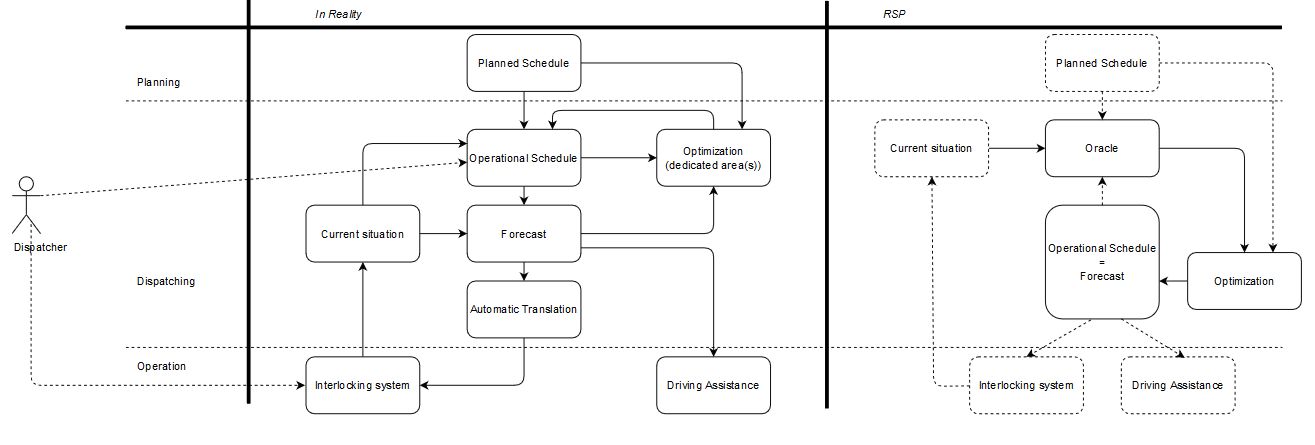
\includegraphics[width=0.9\textheight,angle=90]{introduction_operations.PNG}
  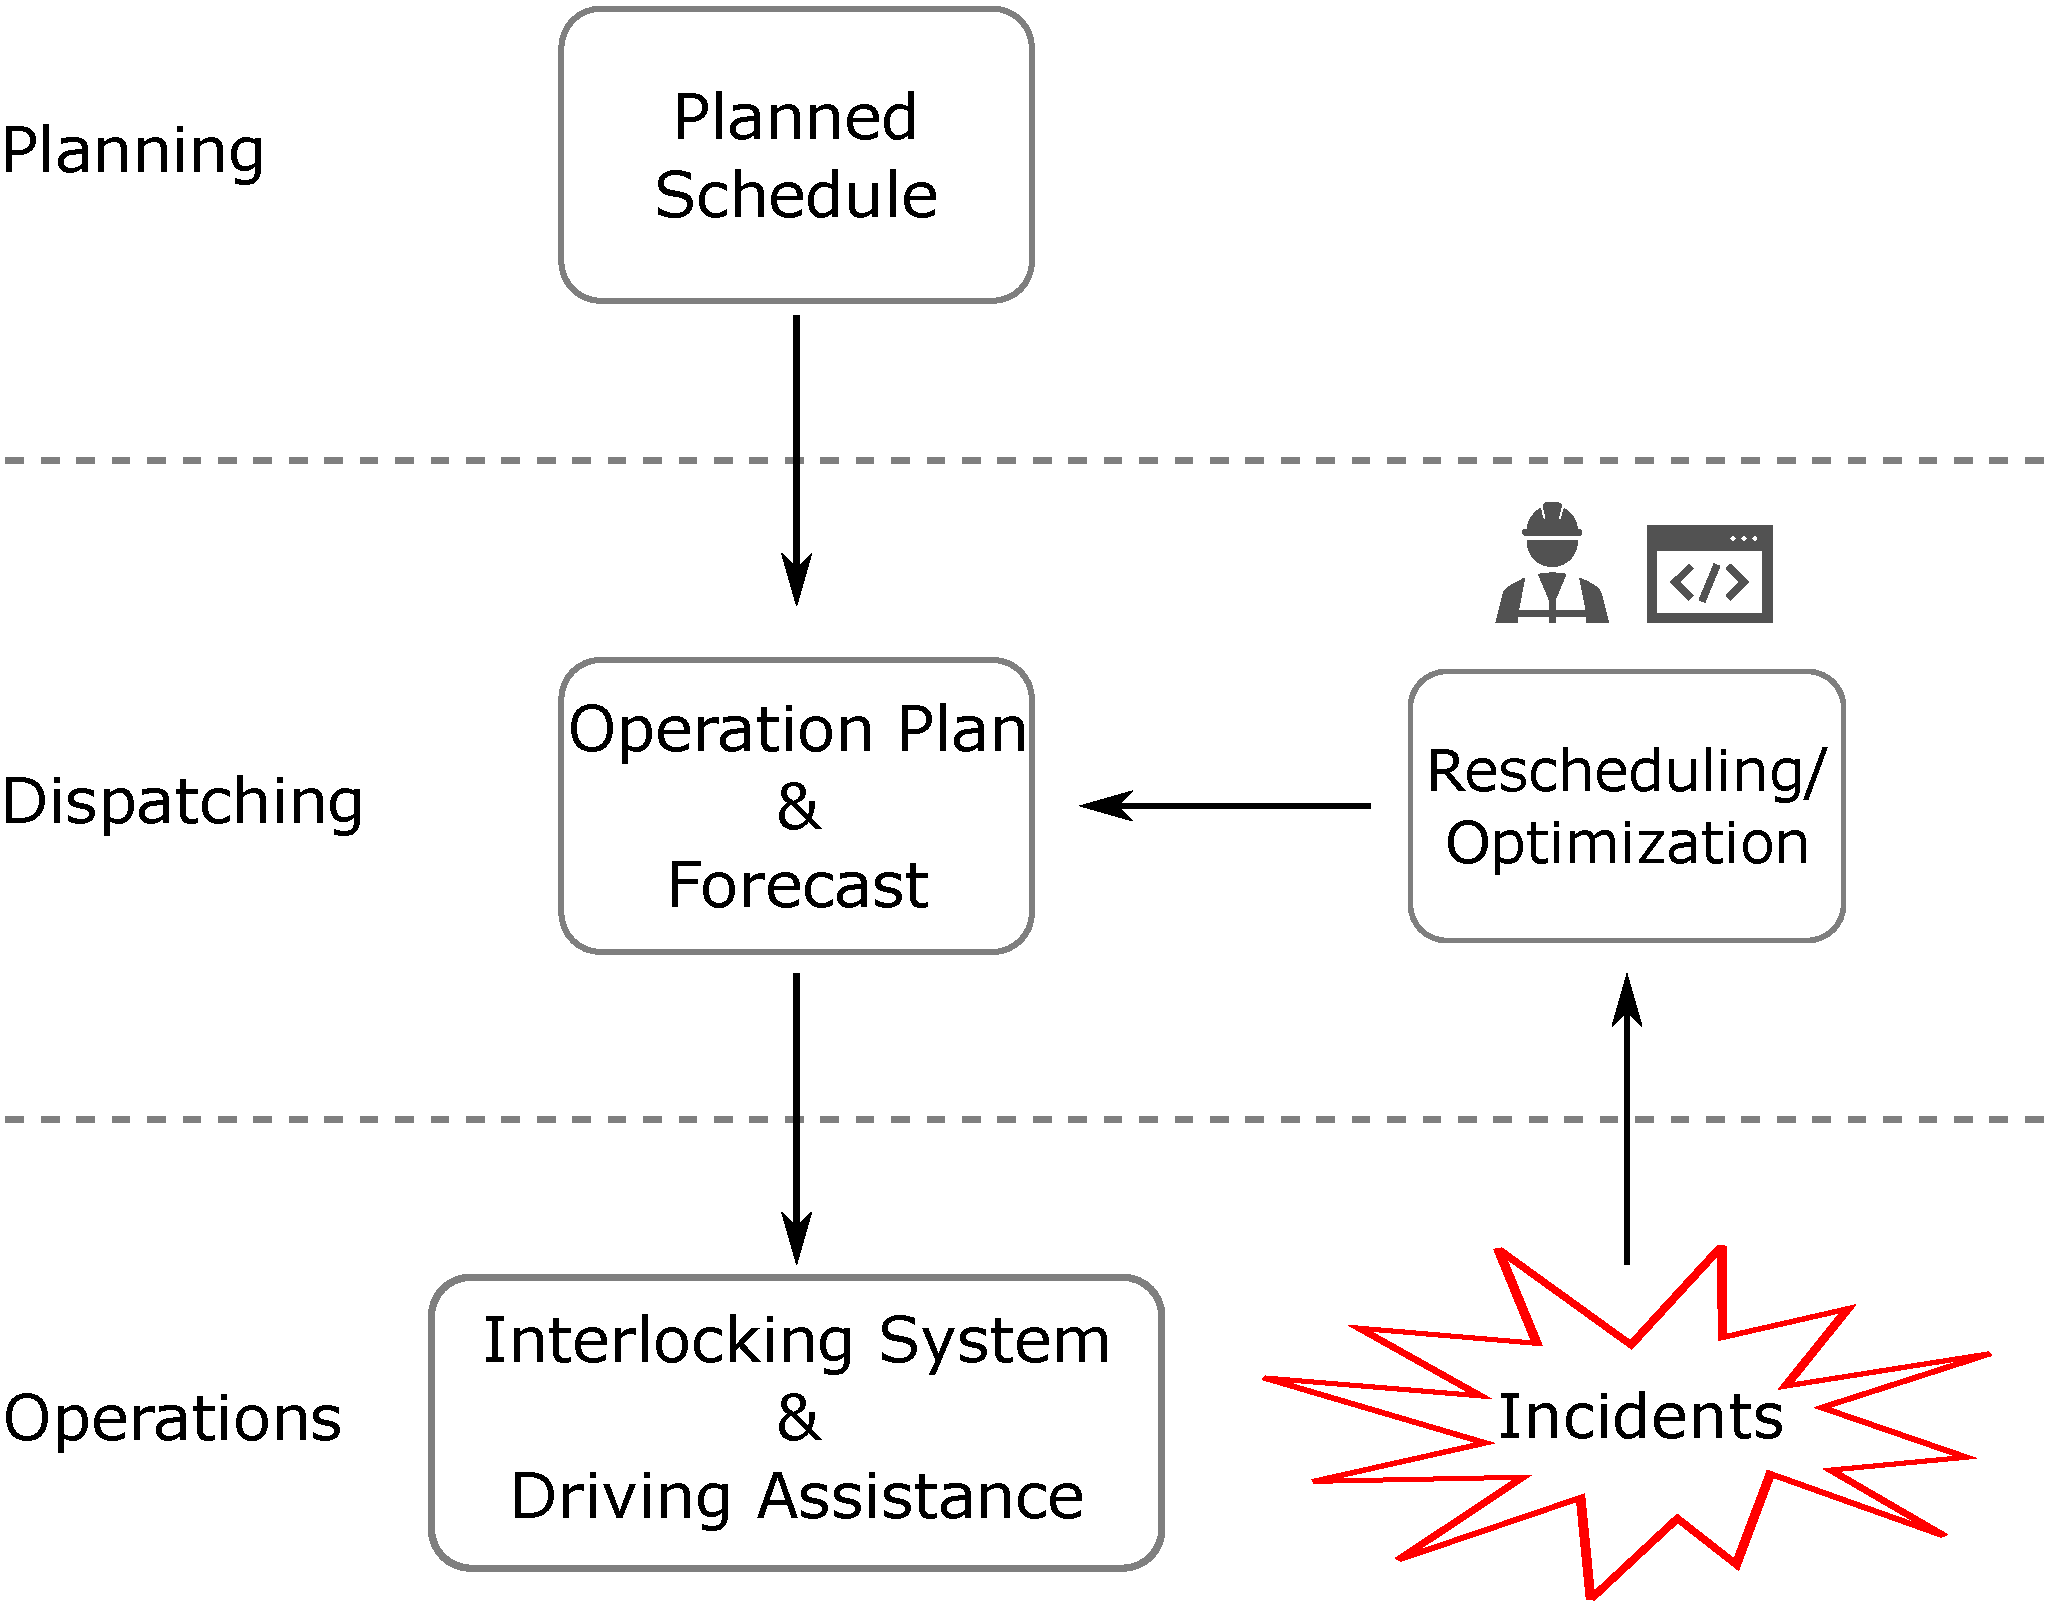
\includegraphics[width=0.8\textwidth]{Figures/rescheduling_schema_heute.pdf}
	\caption{Simplified schema of the rescheduling process during operations. There are three main areas involved: \emph{planning}, \emph{dispatching} and \emph{operation} (interlocking and driving assistance). Dispatchers have access to the current situation and an automated forecast and make decisions at the level of the operational plan, which are then translated either automatically or by dedicated dispatching team members to the interlocking system; some areas are under the control of an automatic optimization system. As time goes on, new elements from the planned schedule will be introduced to the operational schedule and the planned schedule gives also constraints to re-scheduling: passenger trains must not depart earlier than communicated to customers and the service intention may define further hard or soft constraints such as pecuniar penalties for delay or train dropping. The current situation will be reflected in the operational schedule and the forecast.}
	\label{fig:introduction_operations}
\end{figure}
%


The industry state of the art systems efficiently re-compute a traffic forecast for the next two hours, allowing dispatchers to detect potential conflicts ahead of time. The predicted conflicts mostly have to be resolved by humans by explicitly deciding on re-ordering or re-routing based on their experience.

Today, the whole railway system is decomposed into disjoint geographic cells of responsibility as depicted in Figure \ref{fig:geographical_decomposition}. This vastly reduces the complexity within each region and allows human dispatchers to resolve conflicts locally with support of different IT systems. Using structured (e.g. IT system of incident messages) or informal ways (e.g. direct talks with fellow dispatchers) to communicate, different regions can coordinate their dispatching strategies to achieve system wide stability.

%
\begin{figure}[hbtp]
	\centering
  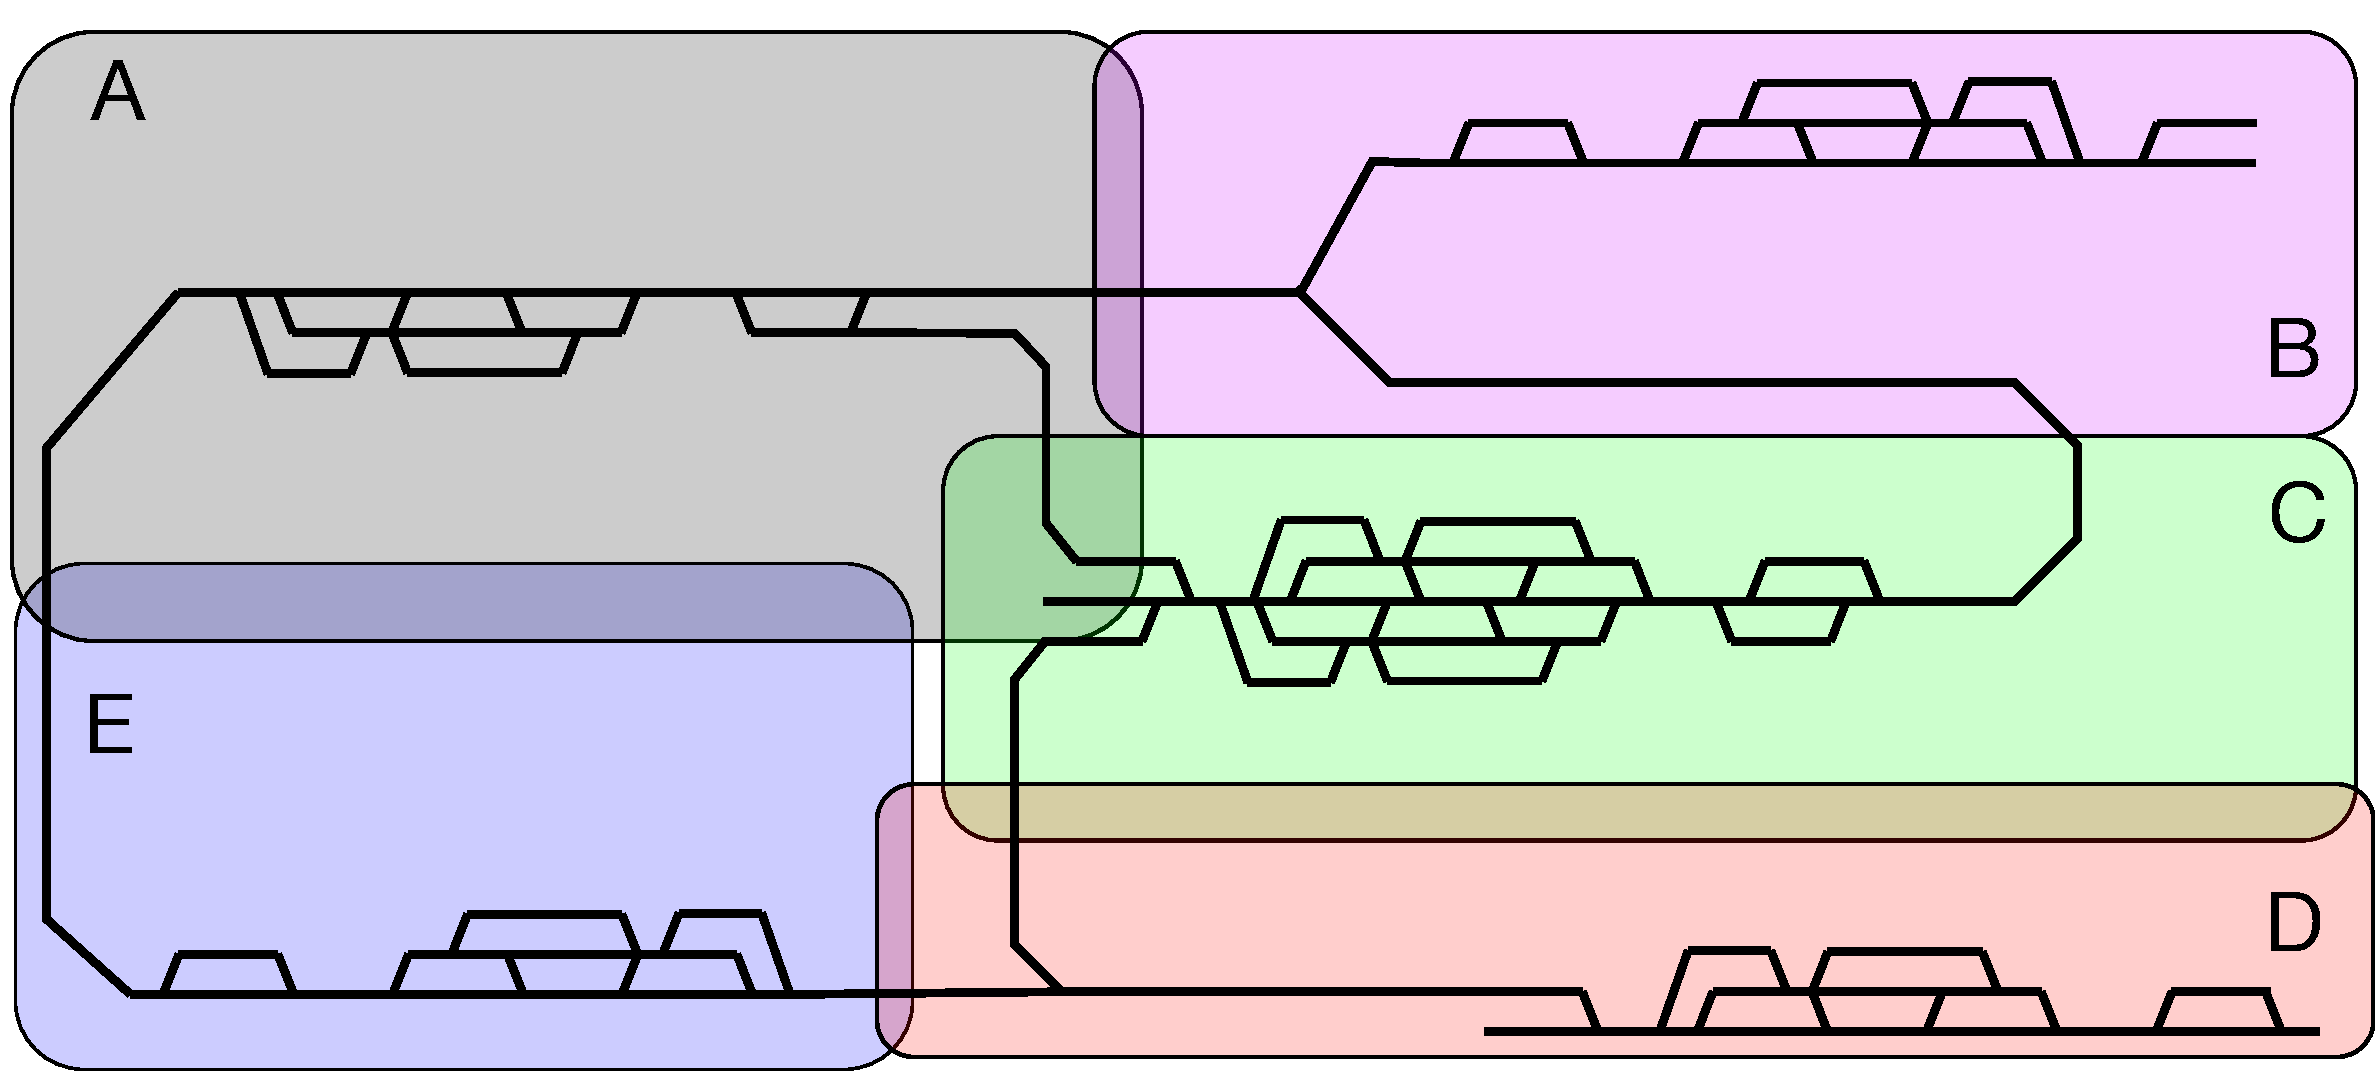
\includegraphics[width=\textwidth]{Figures/disposition_areas.pdf}
	\caption{Due to the vast complexity of a railway network, the re-scheduling task is decomposed into smaller geographical areas (A-E), withiwin which human dispatchers optimize traffic flow. Inter-region coordination is mostly done by informal means of communication such as telephone.}
	\label{fig:geographical_decomposition}
\end{figure}
%

Each region is in itself decomposed according to network properties:

%
\begin{quote}
    [...], a network separation approach is applied to divide the railway network into zones of manageable size by taking account of the network properties, distinguishing condensation and compensation zones. Condensation zones are usually situated near main stations, where the track topology is complex and many different routes exist. As such an area is expected to have a high traffic density, it is also a capacity bottleneck and trains are required to travel through with maximum allowed speed and thus without time reserves. Collisions are avoided by exploiting the various routing possibilities in the station area. Conversely, a compensation zone connects two or more condensation zones and consists of a simpler topology and less traffic density. Here, time reserves should be introduced to improve timetable stability. The choice of an appropriate speed profile is the most important degree of freedom to exploit in these compensation zones. \cite{caimi2009}
\end{quote}

 The complexity of the train rescheduling problem grows exponentially with the number of trains. Hence, there are only a few small so-called condensation areas \cite{caimi2009} that can be operated through automatic systems. For larger areas, we cannot currently find feasible re-scheduling solutions in real-time.


This situation is depicted in a schematic way in Figure~\ref{fig:introduction_compensation}:
%
\begin{figure}[hbtp]
	\centering
  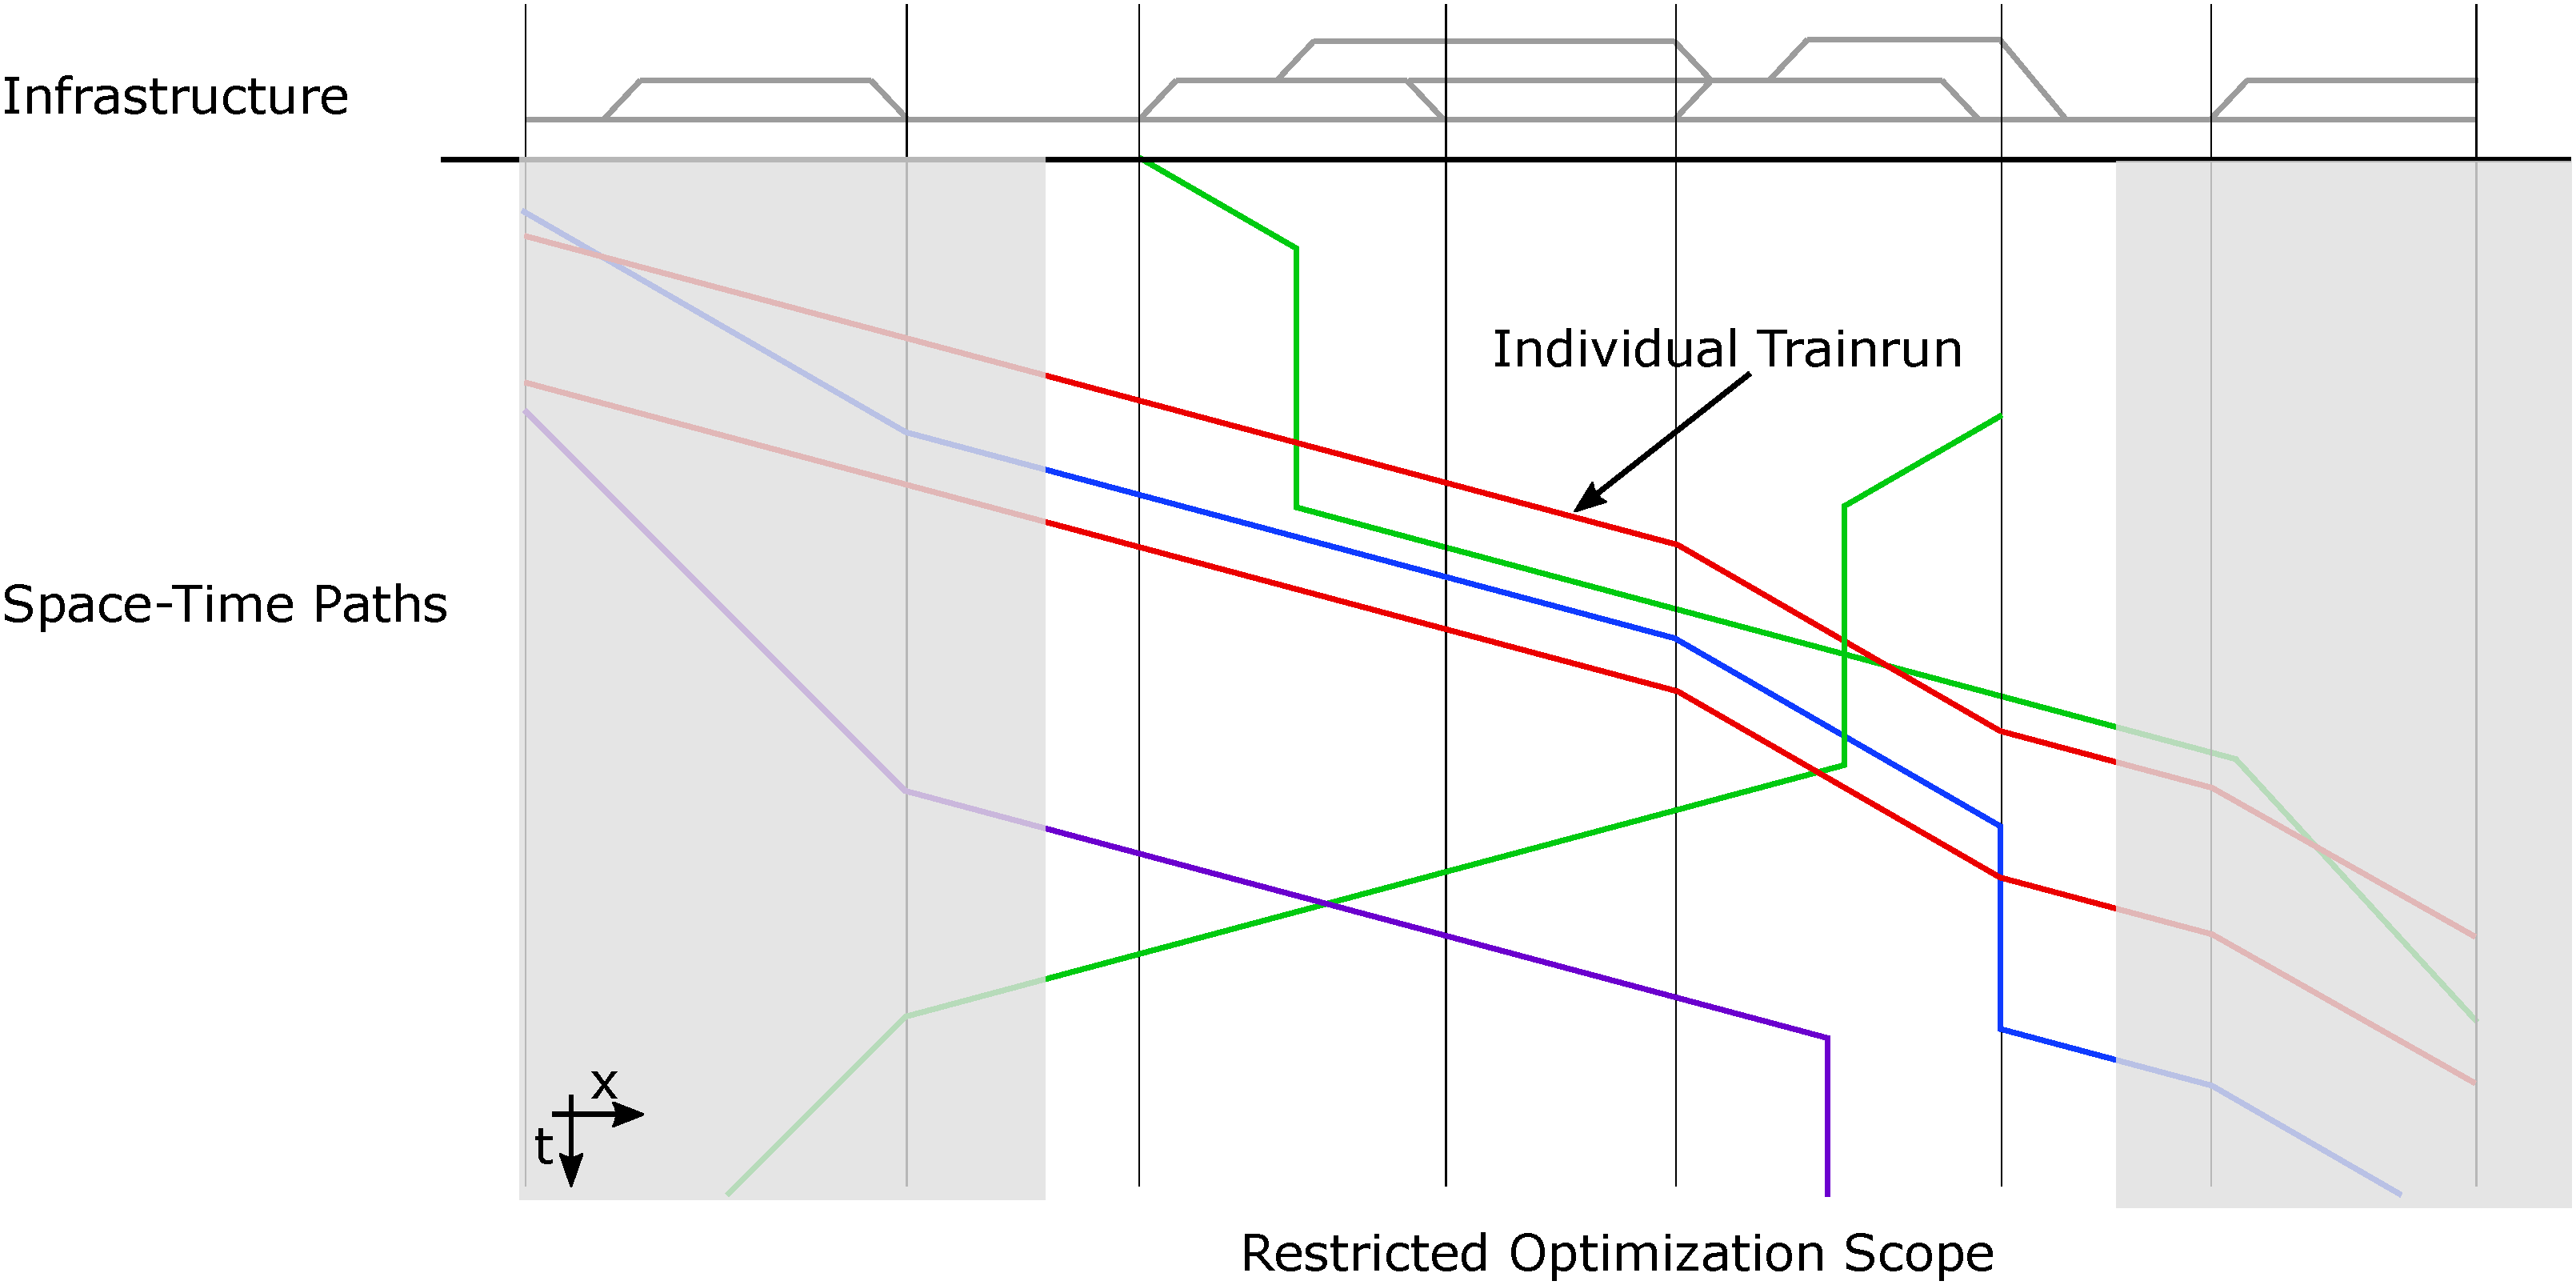
\includegraphics[width=\textwidth]{Figures/rsp_rescheduling_heute.pdf}
	\caption{Real-time rescheduling has so far been applied to restricted geographic areas only. This means that human intervention or buffer times are necessary outside of the optimization scope to guarantee conflict free traffic in the whole network. The limited geographical scope leads to a cost-function that can only locally be minimized and might have negative effects at the whole network scale.}
	\label{fig:introduction_compensation}
\end{figure}

%% EMMA TO WRITE
\subsection{Brief Background on Related Literature}
Railways face a multitude of planning problems, the most important ones can be categorized as routing or scheduling problems \citep{CordEtAl98}. Train scheduling, aka train timetabling, is a tactical planning problem that has been extensively studied in the literature \citep[e.g.,][]{CaprEtAl02,CaccEtAl15}. The schedule is in place over a certain period of time (e.g., a season) and should be robust to minor disruptions \citep[e.g.,][]{LiuDess19, CaccToth12}. More important disruptions caused by, for example, bad weather, infrastructure or equipment failures, induce primary delay on directly affected trains which, in turn, can propagate to other trains in the network.

Real-time railway traffic management focus on controlling the traffic so as to minimize delays. We refer the reader to \cite{Luan19} for a recent and comprehensive literature review.
% %% Improve from here.
The train rescheduling problem (OTHER NAME) focuses on finding mitigating strategies that minimize delay. This is known as the dispatching problem in the literature KEYREF. It is a well-studied problem at the microscopic level REFS. That is, based on a detailed representation of the infrastructure and the train movements. Most computational studies are limited to small infrastructure as the problems are computationally costly to solve. Therefore, the problem are typically solved sequentially at different levels of detail (REF PREVIOUS SECTION). That is, describe sequence. REFCorman study this sequential problem and define constraints that should be enforced at the boarder of ... .

% Train schedule tactical problem
% Full literature review out of the scope of this paper.
% Cite recent thesis for an overview
% In place over an extended period of time. Should be robust to minor disruptions.
% Rescheduling problems when faced with disrputions that induce delay. Objective limit delay propagation.
% Extensive literature on dispatching problem. Microscopic level. Given the level of detail, limited by area, as described in previous section. REFERENCES...
% The problem of coordinating the dispatching between different regions is less studied (Corman, 2012). In this case, macroscopic level. Corman et al., 2012 define constraints at the boarder between areas that the local dispatchers must respect.
% Most computational studies in the literature limited to very small infrastructures.


% EMMA NEXT STEP: Read 7.3 in thesis in detail.
% THEN READ: Fischetti Monaci. Using a general-purpose Mixed-Integer Linear Programming solver for the practical solution of real-time train rescheduling
% Check differences time tabling and scheduling.
[Just ideas for now]
Rescheduling problem for real large-scale networks is impossible to tackle at microscopic level for an entire network. This is why the hierarchical/sequential has been adopted. To the best of our knowledge, the literature is limited to reducing the scope of the dispatching problem to a geographical area of the infrastructure. In this work, we approach the problem in a different way. We propose to reduce scope by identifying which services -- hence a scope in space \emph{and} time) -- that are and will be affected by a disruption. [Literature: detailed/microscopic -- aggregate / macroscopic. We propose to keep the detailed view where relevant in time and space.] The contribution relates to the [COORDINATION name?] problem that has been less studied than the [microscopic dispatching problem -- introduce name earlier]. [Trade-off: number of areas and complexity of coordination problem. Aim of our work is to be able to deal with larger areas.] The idea is not to replace the existing solution approaches. Rather, we propose this as an alternative way to reduce problem scope that could potentially be combined with different models and solution approaches from the literature.


%% EMMA TO WRITE
\subsection{Objectives} \label{sec:objectives}
%% Add the objectives here that are now described in the abstract. The abstract can be shortened.

% Motivation / observation. Use the fact that schedule is in place over quite a long period of time...

% The objective is to complement existing work on train rescheduling problem.



%%%%%%%%%%%%%%%%%%%%%%%%%%%%%%%%%%%%%%%%%%%%%%%%%%%%%%%%%%%%%%%%%%%%%%%%%%
%%%%%%%%%%%%%%%%%%%%%%%%%%%%%%%%%%%%%%%%%%%%%%%%%%%%%%%%%%%%%%%%%%%%%%%%%%
\section{Research Approach}\label{sec:researchapproach}
%%%%%%%%%%%%%%%%%%%%%%%%%%%%%%%%%%%%%%%%%%%%%%%%%%%%%%%%%%%%%%%%%%%%%%%%%%
%%%%%%%%%%%%%%%%%%%%%%%%%%%%%%%%%%%%%%%%%%%%%%%%%%%%%%%%%%%%%%%%%%%%%%%%%%
In this work we propose a novel solution approach to overcome the limited spatial restrictions of automated algorithmic re-scheduling by extracting the core problem variables from the original full problem formulation. We propose to utilize the strength of state-of-the-art machine learning algorithms to extract the core problem, which in turn is solved by any known optimizer such as Simplex or ASP. We test our novel research approach through experiments on a simplified railway simulation.


Our playground implementation is an abstraction of real railway traffic (see Section~\ref{subsec:playground} below), shown in Figure~\ref{fig:introduction_operations}: we only consider an operational plan and a single incident (malfunction) and try to re-schedule such that we have a conflict-free plan again that stays close to the (published) planned schedule. We hint at a fully automatic re-scheduling loop as follows:

\begin{enumerate}
    \item operational plan is updated according to real time data
    \item core problem scope is extracted from operational plan
    \item optimizer solves core problem and generate new operational plan
    \item repeat.
\end{enumerate}

%%%%%%%%%%%%%%%%%%%%%%%%%%%%%%%%%%%%%%%%%%%%%%%%%%%%%%%%%%%%%%%%%%%%%%%%%%
\subsection{Core idea}\label{subsec:coreidea}
%%%%%%%%%%%%%%%%%%%%%%%%%%%%%%%%%%%%%%%%%%%%%%%%%%%%%%%%%%%%%%%%%%%%%%%%%%

We assume that any re-scheduling problem that arises within the global railway system can be reduced to a much smaller re-scheduling problem consisting only of a subset of active trains at any given time, we refer to this as the \emph{core problem}. In contrast to current models we do not follow a spatial decomposition according to network properties but rather investigate the possibility of predicting the relevant core problem given a schedule and a malfunction.

In other words, we assume that it is possible to predict the scope of influence from a given disturbance and that a feasible solution can be found within that scope while keeping the operational schedule fixed outside. The scope consists of:
\begin{itemize}
    \item Departure times of trains
    \item Routes of trains
\end{itemize}
and hence spans both space and time, in contrast to spatial decomposition.


We present an exploratory study of the following questions:
\begin{enumerate}
\item Is it possible to predict the trains that will be affected by a given disruption based on the problem structure, historical or simulated data?
%it is possible to predict the affected time-space area, either from the problem structure or from historic data
\item Can we compute solutions to the restricted problem scope much faster than the full scope?
%solutions within the restricted problem scope can be found much faster than the full railway system
\item Are the solutions to the restricted problem scope of similar quality to those of the full problem?
%feasible solutions within the restricted problem scope show a similar quality to full network solutions.
\end{enumerate}

Our approach combines Operations Research and Domain-specific Learning to get the best of both worlds: a ``Scope predictor'' is able to predict the ``impact'' of a disturbance, with or without a knowledge base learnt by training; we hope the scope-predictor could predict which trains and which departures are or could be affected by the disturbance based on past decisions. This piece of information from the scope-predictor then constrains the search space for the solver or at least drives its search more efficiently (driving the branching process).

%%%%%%%%%%%%%%%%%%%%%%%%%%%%%%%%%%%%%%%%%%%%%%%%%%%%%%%%%%%%%%%%%%%%%%%%%%
\subsection{Synthetic Playground}\label{subsec:playground}
%%%%%%%%%%%%%%%%%%%%%%%%%%%%%%%%%%%%%%%%%%%%%%%%%%%%%%%%%%%%%%%%%%%%%%%%%%

We now give a short introduction to our playground implementation (G4) and its limitation with respect to real-world features.
\begin{description}
\item[Synthetic Infrastructure and Simplified Resource Model] \hfill \\
We use the FLATland toolbox \cite{aicrowdFLATland} to generate a grid world infrastructure consisting of railway elements in 2D grid. Each railway element occupies a square cell in this grid. The railway element defines the orientation depended possible transitions of a train to the four direct neighbouring cells (e.g. switches allow for different transitions depending on the orientation of a train on the switch). Infrastructure details can be found in section \ref{subsubsec:infrastructuregeneration}
\item[Synthetic Timetable and Train Dynamics] \hfill \\
Given a specific infrastructure we generate a simplified synthetic schedule with the following constraints:
\begin{itemize}
    \item Every train has one single source and target, no intermediate stops, as provided by the FLATland toolbox \cite{aicrowdFLATland}.
    \item Every train has a constant speed (which may be different from train to train), as provided by the FLATland toolbox \cite{aicrowdFLATland}.
    \item The schedule (departure and passing times at all cells) is generated such that the sum of travel times of all trains is minimized within a chosen upper bound.
    \item There are no time reserves in the schedule, which means that trains cannot reduce delay during their journey.
    \item There is no distinction between published timetable and operational schedule, we only have an operational timetable; in reality, trains must not depart earlier than published.
    \item There are no scheduled connections between trains or vehicle tours (turnrounds).
\end{itemize}
\item[Synthetic route alternatives] \hfill \\
We use k-shortest paths from source to target as list of route alternatives; path cycles are not allowed. In reality, the choice and prioritization of route alternatives is intricate.
\item[Simple Disturbance Model] \hfill \\
We simulate one train $a$ being stopped for $d$ discrete time steps at some time $t$ and call this a malfunction $M=(t,d, a)$;  This setup is shown in Figure~\ref{fig:introduction_no_loop}. In reality, the delay might not be known or only probabilities can be assumed and multiple disturbances can occur independently.
\end{description}
%
\begin{figure}[hbtp]
	\centering
  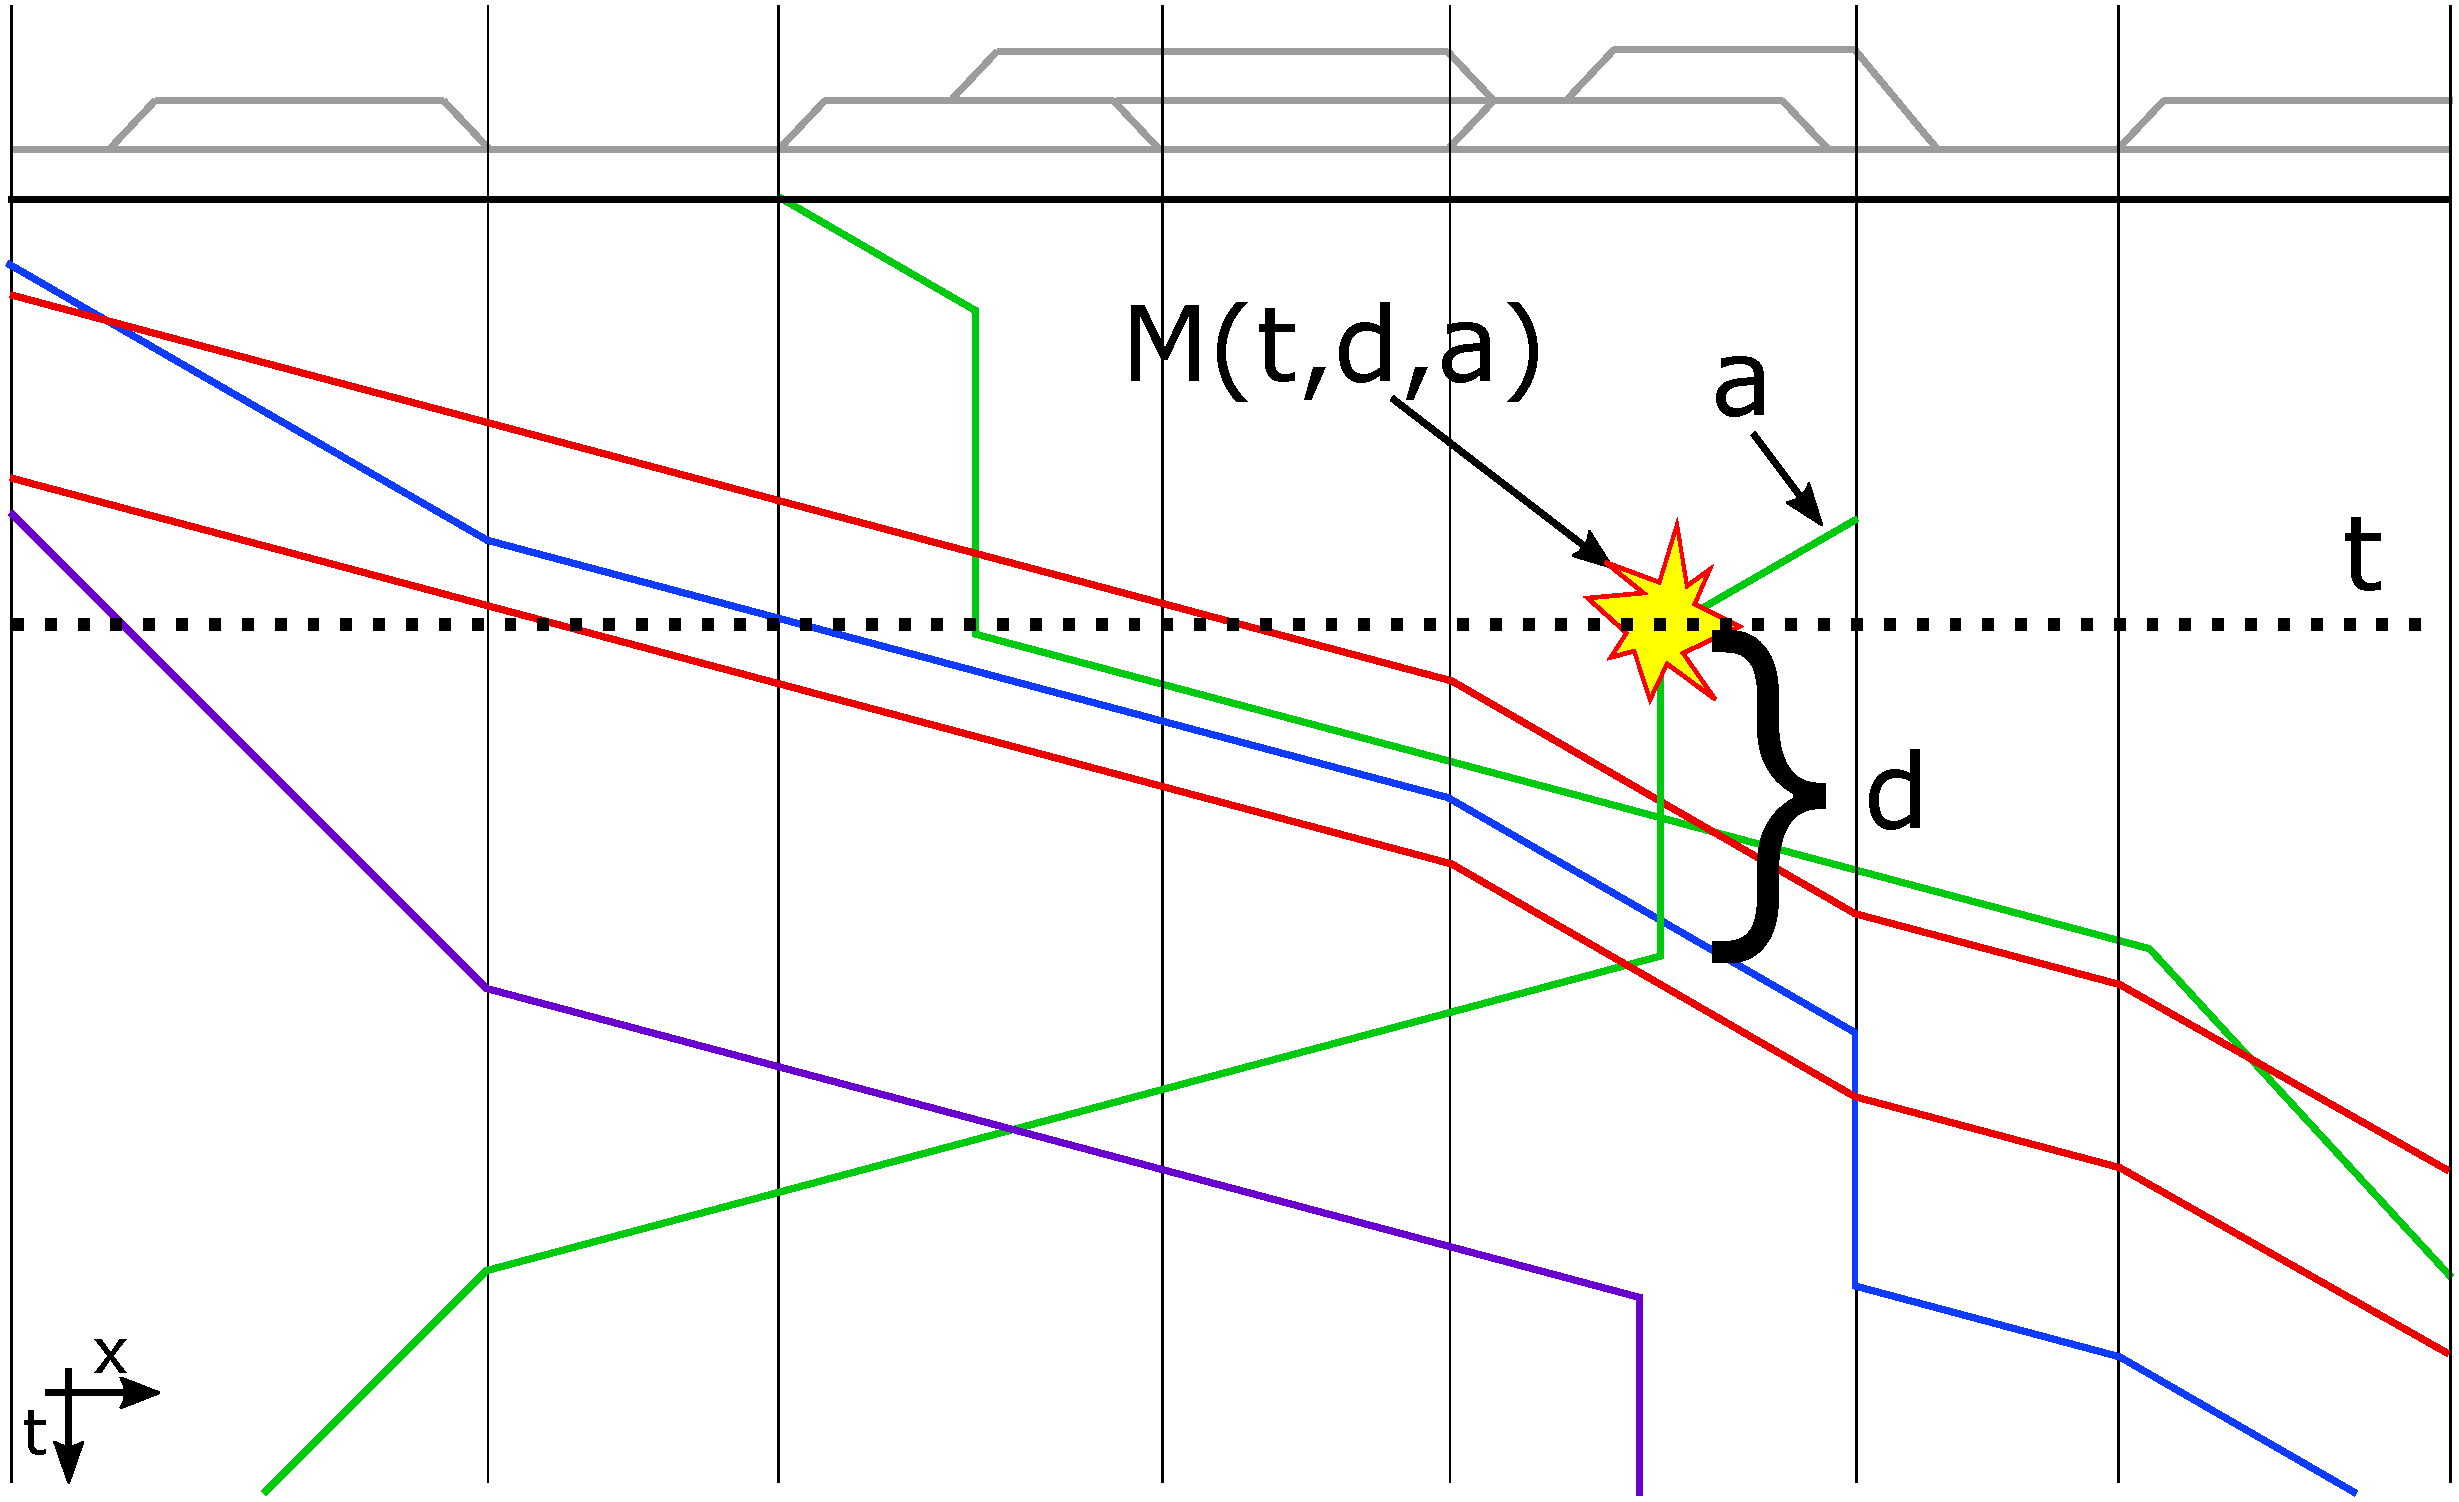
\includegraphics[width=\textwidth]{Figures/malfunction_generation.pdf}
	\caption{This figure illustrates a simple operations plan with 6 trains on a small infrastructure. A single malfunction $M(t,d,a)$ occurs for agent $a$ at time $t$ with a total duration of $d$ time steps. In reality of course there exists many different disturbances in the network which we will discuss further in Section~\ref{subsec:malfunction_variation}}
	\label{fig:introduction_no_loop}
\end{figure}

%%%%%%%%%%%%%%%%%%%%%%%%%%%%%%%%%%%%%%%%%%%%%%%%%%%%%%%%%%%%%%%%%%%%%%%%%%
\subsection{Reduction in Space and Time}\label{subec:slicing}
%%%%%%%%%%%%%%%%%%%%%%%%%%%%%%%%%%%%%%%%%%%%%%%%%%%%%%%%%%%%%%%%%%%%%%%%%%




The main idea of problem scope reduction is shown in Figure~\ref{fig:introduction_time_space}, where the scoper predicts what parameters in time and space are relevant to solve the core problem caused by the malfunction.

%
\begin{figure}[hbtp]
	\centering
  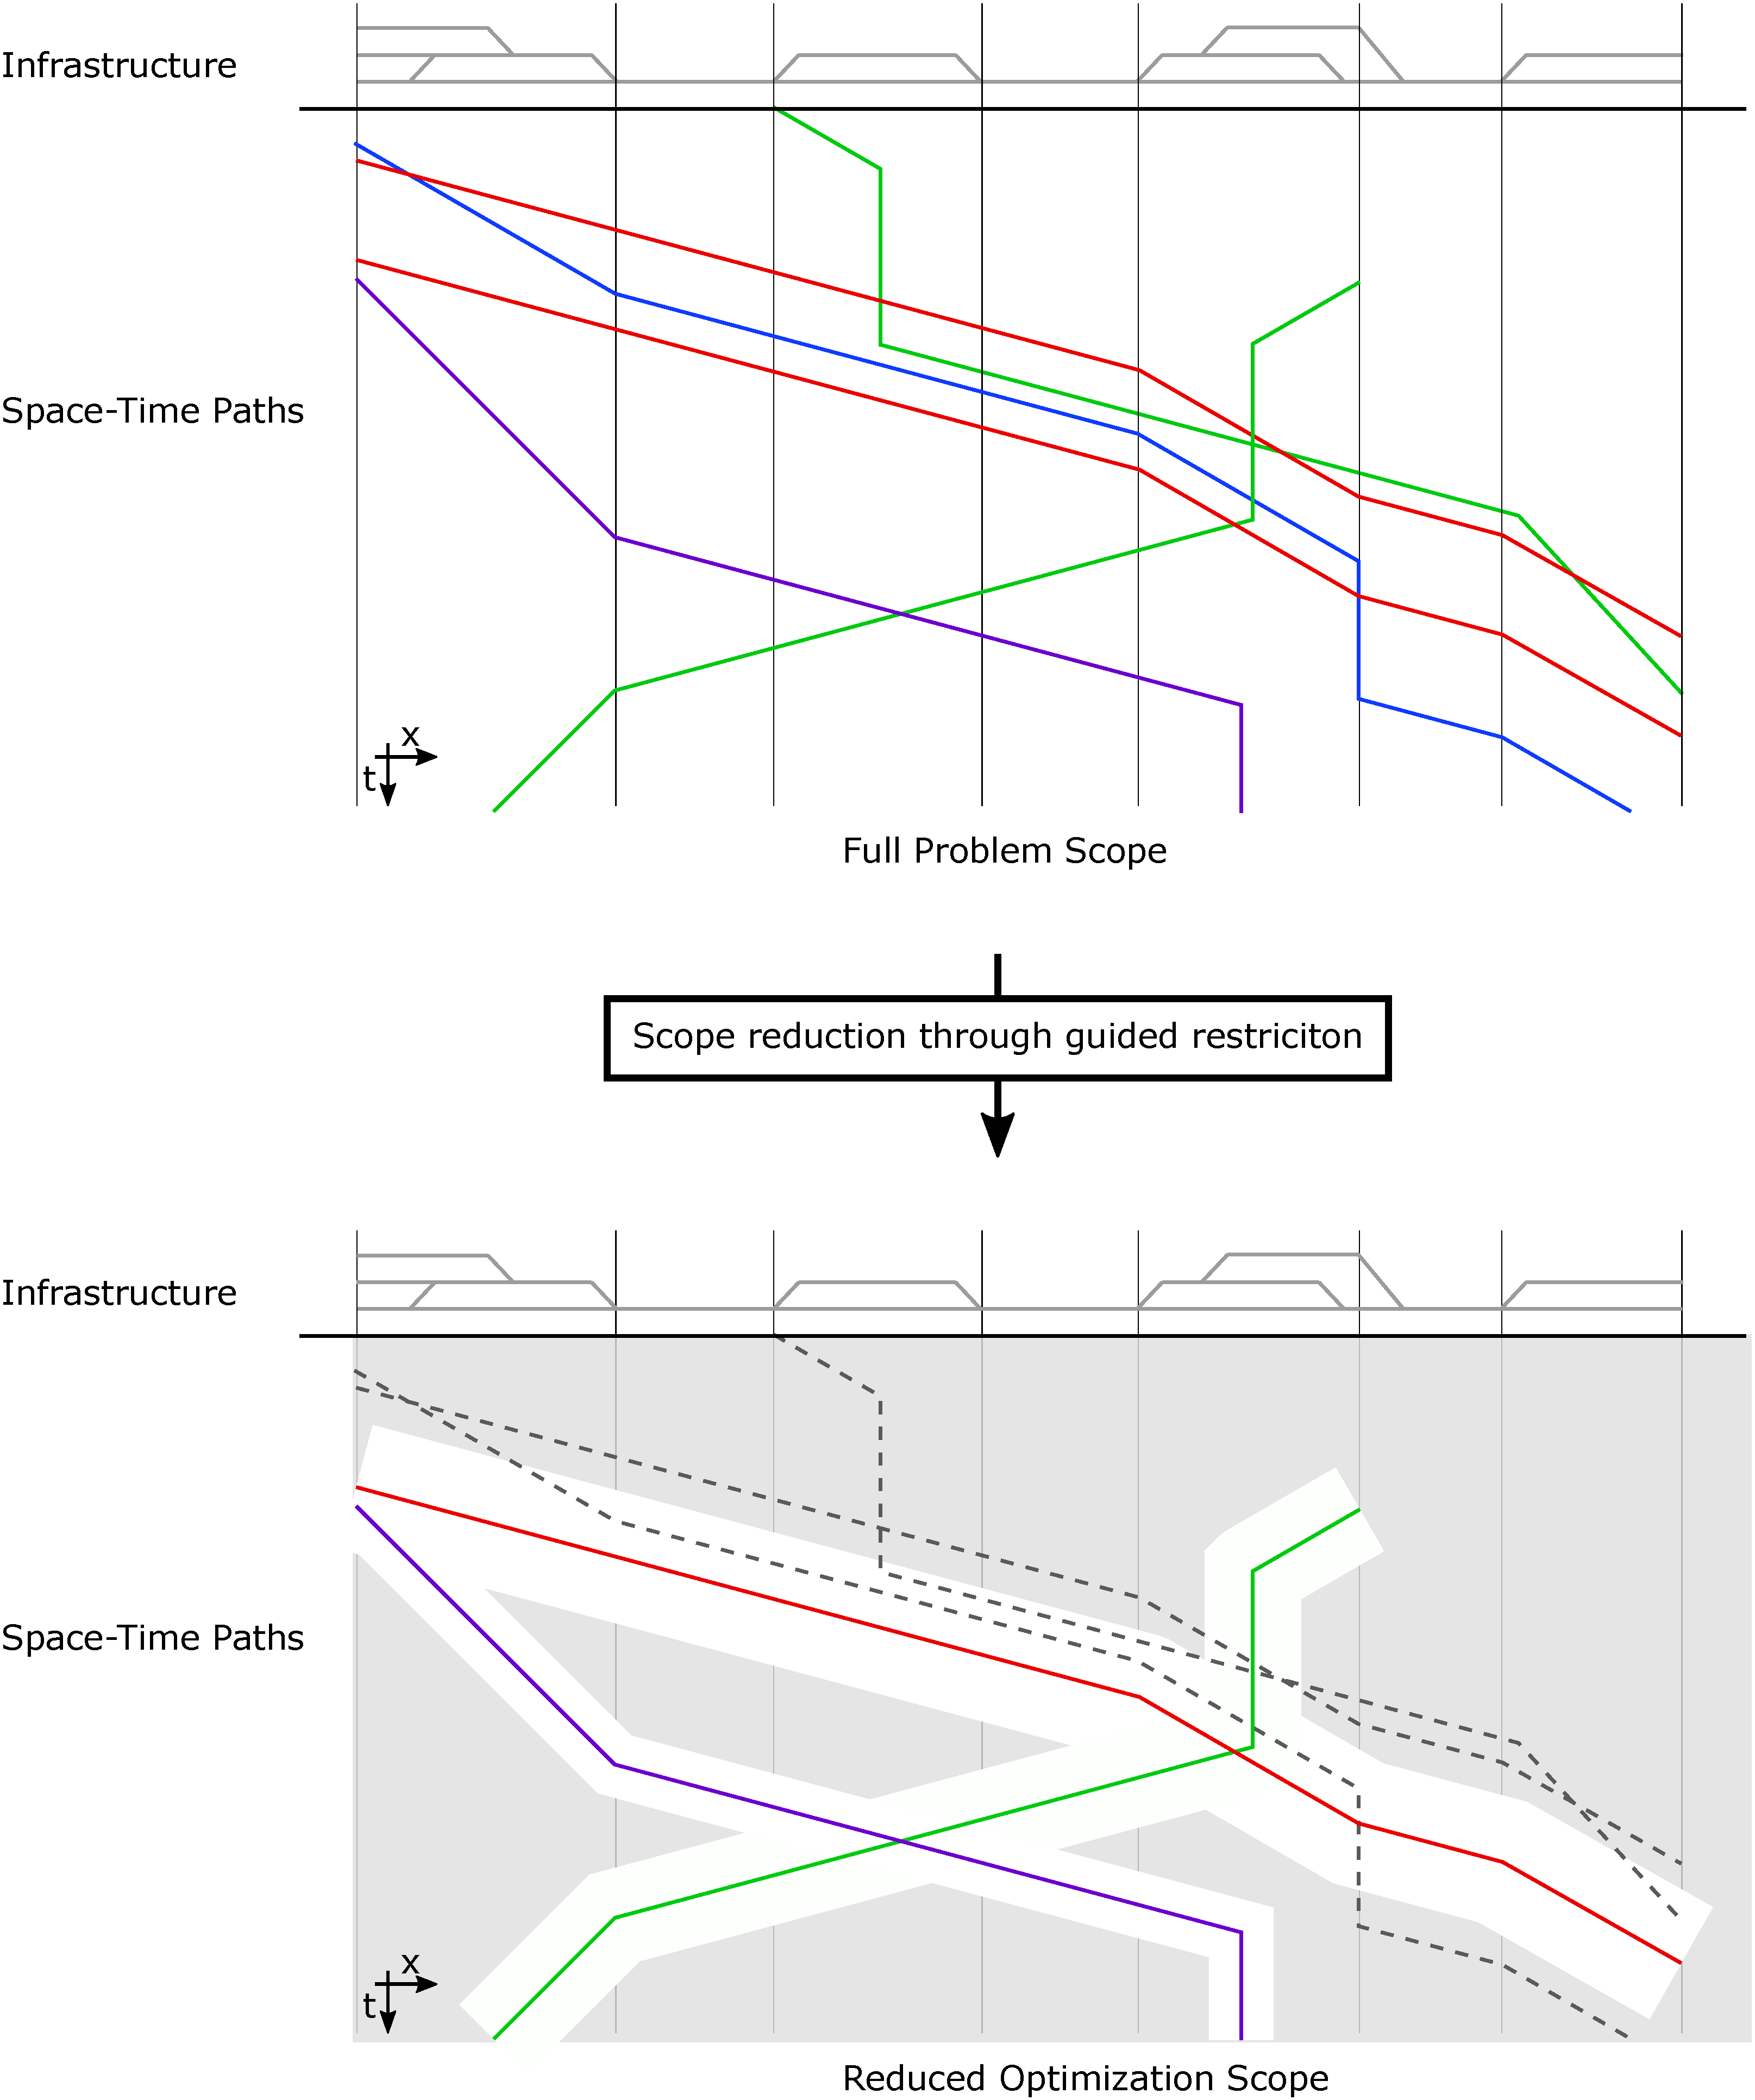
\includegraphics[width=\textwidth]{Figures/rsp_rescheduling_rsp.pdf}
	\caption{The scope reducer condenses the initial full problem description to the core problem in the time-space parameters. This vastly reduces the search space of an optimizing algorithm.}
	\label{fig:introduction_time_space}
\end{figure}

%%%%%%%%%%%%%%%%%%%%%%%%%%%%%%%%%%%%%%%%%%%%%%%%%%%%%%%%%%%%%%%%%%%%%%%%%%
\subsection{Online and Offline Scoping}\label{subec:online_offline}
%%%%%%%%%%%%%%%%%%%%%%%%%%%%%%%%%%%%%%%%%%%%%%%%%%%%%%%%%%%%%%%%%%%%%%%%%%

We distinguish two types of scopes:
We distinguish between two classes of scopes:
\begin{description}
\item[online] the scoper does not have access to a full re-schedule solution\footnote{More precisely, online scopers know at most how many agents have changed but not which ones, see below offline delta weak vs. online random.}
\item[offline] the scoper has access to a full re-schedule solution
\end{description}
%
The rationale of offline scoping depending on a is shown in Figure~\ref{fig:online_offline}.
\begin{figure}[hbtp]
	\centering
  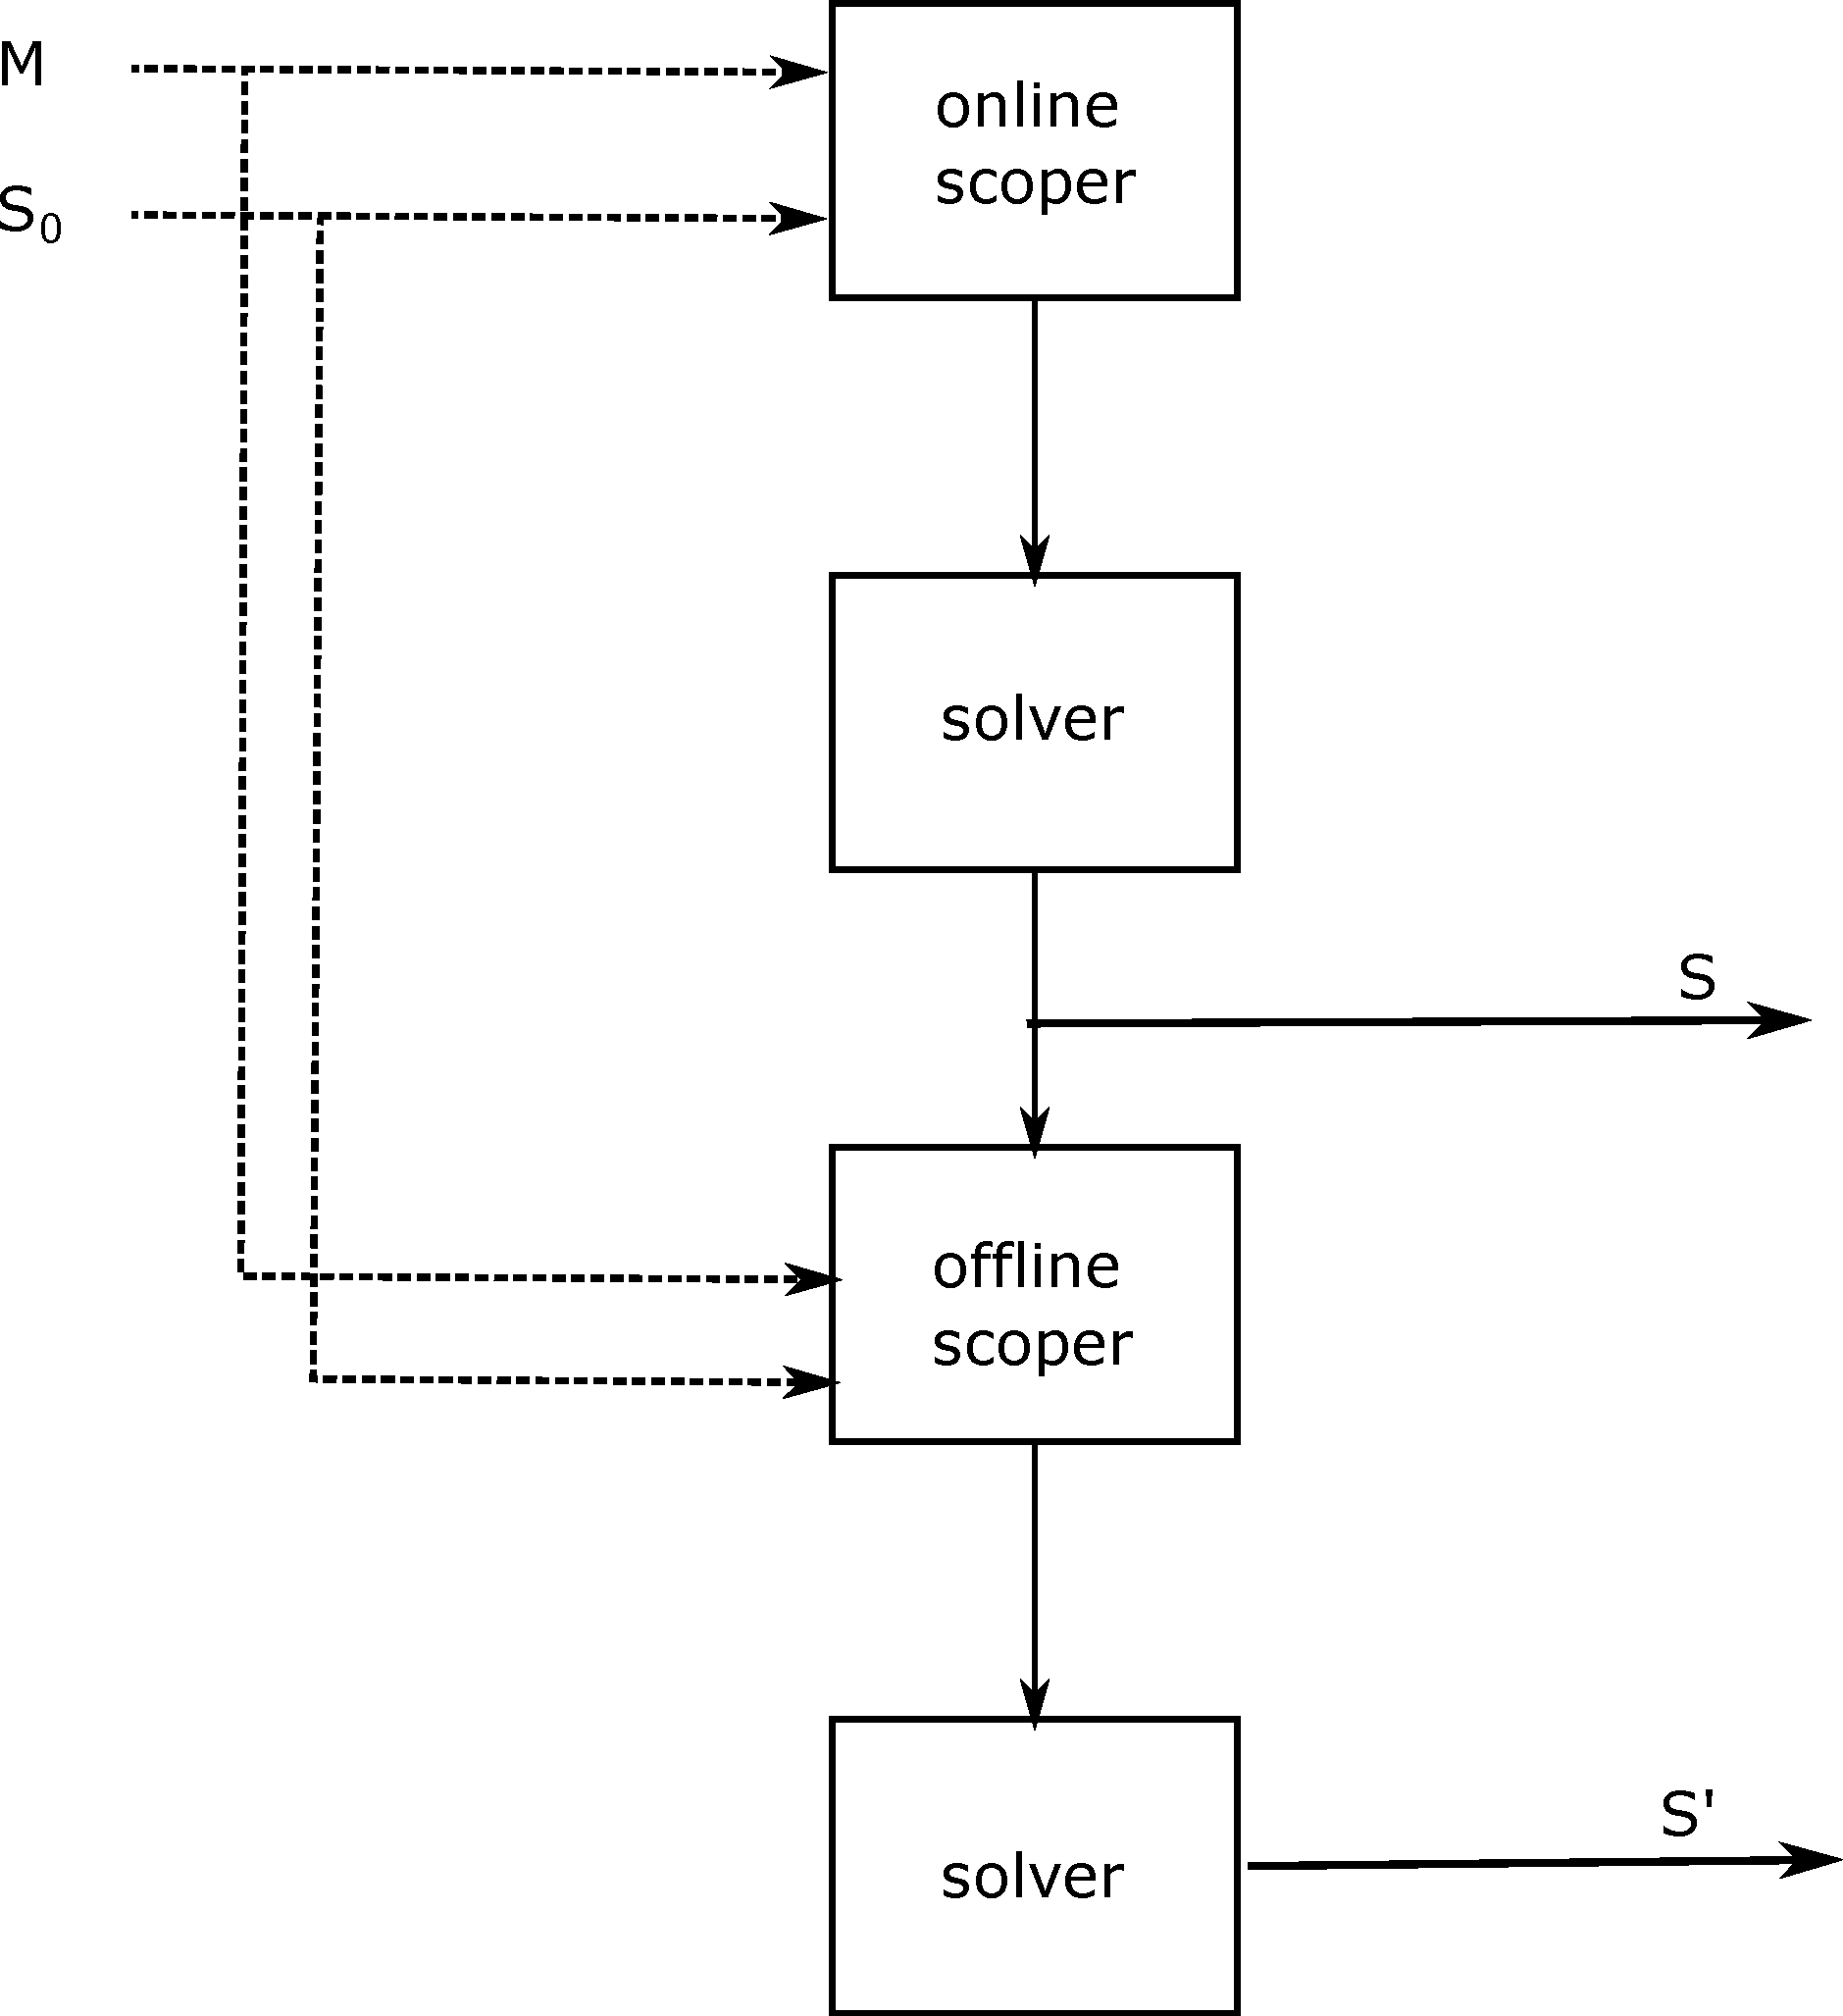
\includegraphics[width=0.8\textwidth]{Figures/02_research_approach/online_offline.pdf}
	\caption{Signal-flow diagram for online and offline scoping. It shows the online re-schedule $S$ and the the offline re-schedule $S^\prime$. It shows that offline scoper takes the online schedule as an additional in addition to the malfunction $M$ and the initial schedule $S_0$.}
% https://mitpress.mit.edu/sites/default/files/sicp/full-text/book/book-Z-H-24.html#%_sec_3.5.4
	\label{fig:online_offline}
\end{figure}



We will consider the following problem scope reduction schemes (scopers):
\begin{description}
\item[online\_unrestricted] this scoper does not restrict the re-scheduling problem, it is the ``full'' re-scheduling problem with ``empty'' scope reduction, supposed to give a trivial lower bound on speed-up with respect to the solver; this excludes unreachable alternative paths after the malfunction
\item[offline\_fully\_restricted] this scoper takes the re-scheduling solution from the online\_unrestricted scoper as its scope. This gives a trivial upper bound on speed-up with respect to the specific solver since it measures the specific solver's overhead.
\item[offline\_delta]  this scoper reduces the  scope to the difference between the initial schedule and the online\_unrestricted solution,
\begin{itemize}
    \item only edges from either schedule or online\_unrestricted are allowed;
    \item if location and time is the same in schedule and full-reschedule, then we stay at them
\end{itemize}
supposed to give a non-trivial but unrealistic baseline on speed-up (upper-bound for non-trivial scopers); in this case, the solution from online\_unrestricted is contained in the solution space, so we expect the same (or an equivalent solution modulo costs) to be found.
\item[offline\_delta\_weak] this scoper gives a lose delta by opening up the same as online\_unrestricted for changed agents. This gives a first impression how much speed-up we gain by scoping on a train-by-train basis. We expect this to work reasonably well in sparse infrastructures / schedules, but less so in denser infrastructure/schedules, which do not separate well the effect of a malfunction. This might give us hints as to how well a scoper needs to work (with respect to a solver) in order to achieve desired speed-ups.
\item[online\_route\_restricted] this scoper restricts the re-scheduling problem to the routes chosen in the schedule, but giving time flexibility, suppposed to show the influence of re-routing on computation times and solution quality
\item[online\_transmission\_chains\_fully\_restricted] this scoper uses a simple delay propagation algorithm along the scheduled paths to predict which trains will be affected by the malfunction, keeping unaffected trains exactly at their path and times, supposed to show a baseline speed-up (lower bound for non-trivial scopers); we expect the solution quality to deterioriate if there are false negatives.
\item[online\_transmission\_chains\_route\_restricted] in contrast to the precedent scoper, unaffected agents are given time flexibility (they are constrained to use the same path as in the schedule, though)
\item[online\_random] this scoper randomly chooses affected agents, giving no re-routing flexibility to the unaffected trains, supposed to show that the problem of predicting which agents will be affected is not trivial: this is a sanity check online scoping: if we predict affected trains randomly, we expect solutions to be worse than the ones found by the other scopes or; furthermore, we have time flexibility to trains not chosen since for example if a train is scheduled to pass through the malfunction train during its malfunction and is not opened, there is no solution even if we enlarge time windows on the chosen affected agents.
\end{description}

These scopers will be introduced formally with pseudo-code below in Section~\ref{subsec:scopers}.


%%%%%%%%%%%%%%%%%%%%%%%%%%%%%%%%%%%%%%%%%%%%%%%%%%%%%%%%%%%%%%%%%%%%%%%%%%
\subsection{Research Programme: two Hypotheses }\label{subec:hypotheses}
%%%%%%%%%%%%%%%%%%%%%%%%%%%%%%%%%%%%%%%%%%%%%%%%%%%%%%%%%%%%%%%%%%%%%%%%%%
We will now detail the general line of argument of Section~\ref{subsec:coreidea} by introducing two hypotheses
\begin{description}
\item [Hypothesis 1 (H1)] : if we have access to an offline solution of the re-scheduling problem given unbounded resources, we can design an offline scope reduction that allows for a large speed-up in solution time (see below, Section~\ref{subec:H1}); by this, we achieve goal \textbf{G2}.
\item [Hypothesis 2 (H2)] it is possible to design an online scope reduction, either from the problem structure or from historic data, which achieves similar speed-up factors as H1 (see below, Section~\ref{subec:H2}); by this, we would over-achieve goal \textbf{G3}.
\end{description}

\subsubsection{Hypothesis H1}\label{subec:H1}

Hypothesis 1 is a sanity hypothesis: if we cannot achieve a substantial speed-up with the offline\_delta scoper, the whole approach must be re-evaluated and adjusted.

Consider Figure~\ref{fig:introduction_H1}:
%
\begin{figure}[hbtp]
	\centering
  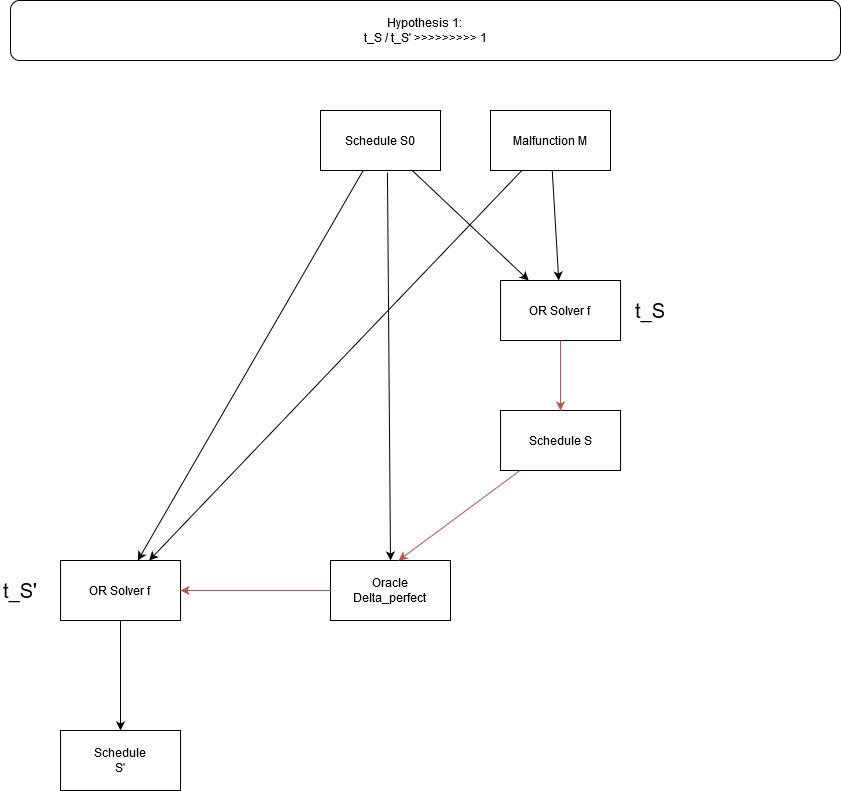
\includegraphics[width=0.9\textwidth]{introduction_H1.png}
	\caption{Rationale of hypothesis H1.}
	\label{fig:introduction_H1}
\end{figure}
%
The initial schedule $S_0$ and a malfunction $M$ are passed to an OR solver which is given unbounded time to solve the model to optimality; the resulting re-schedule is $S$.

If we compare the initial schedule $S_0$ and the re-schedule $S$, we can take the differences ($offline\_delta$) and define a new and reduced problem scope as follows:

\begin{itemize}
    \item every temporal difference between $S_O£$ and $S$ at the same (partial) route opens up timing flexibility: the (partial) routes are kept fixed, but the time variable becomes part of the new problem scope.
    \item every (partial) route  difference between $S_0$ and $S$ opens up routing flexibility: routing and time variables become part of the new problem scope.
\end{itemize}
We will describe this in more detail below in Section~\ref{subsubsec:scope_online_unrestricted}.

We investigate if an OR solver $f$, given the reduced problem scope, has a much shorter solution time $t\_{S^\prime}$  compared to the time $t\_S$ for the full problem without the restriction.

The rationale of this hypothesis is non-general and asymmetric:
%
\begin{itemize}
    \item
    \emph{non-general}: if we show the speed-up for one particular OR solver, this does not mean that the information can be exploited by every other OR solver for speed-up. However, we conjecture that general setup may be applicable to other OR solvers and models, where the exact content of the Oracle's "hint" passed to the solver might differ. We might strengthen this conjecture by comparing with
\item
    \emph{asymmetric}: If we cannot show the speed-up for one particular solver, this does not exclude that the approach might work with a different OR solver and its particular shape of ``perfect information''. We might need to consider a different OR solver for our exposition.
\end{itemize}



\subsubsection{Hypothesis H2}\label{subec:H2}
Hypothesis 2 asks whether we can build an oracle that provides a considerable speed-up with access only to iformation at the current time.

Consider Figure~\ref{fig:introduction_H2}:
%
\begin{figure}[hbtp]
	\centering
  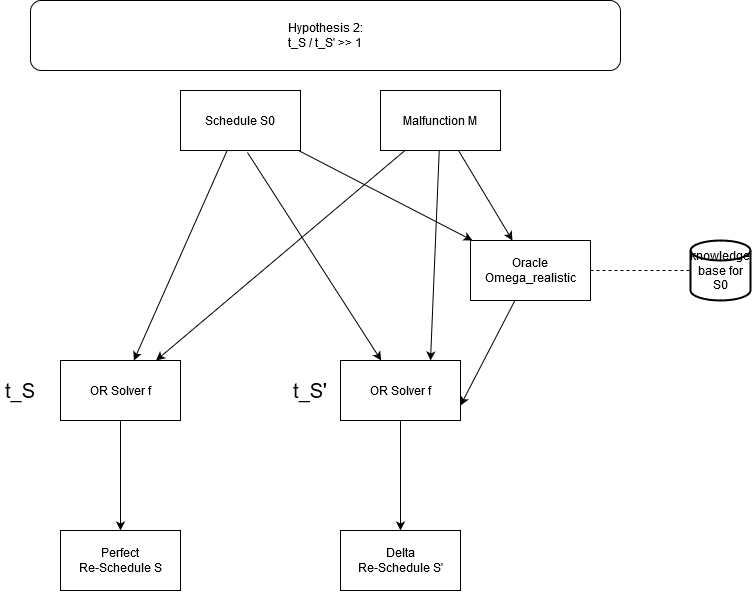
\includegraphics[width=0.9\textwidth]{introduction_H2.png}
	\caption{Rationale of hypothesis H2.}
	\label{fig:introduction_H2}
\end{figure}
%
Our scoper $Omega\_realistic$ only has access to the current information and possibly its knowledge base, not to the perfect re-schedule for the current situation. Is such a scoper able to reduce the scope to a degree that allows for a speed-up $t\_S / t\_S' >> 1$?

The implementation of such a scoper $Omega\_realistic$ is outside the scope of this research, but we
\begin{itemize}
\item report on some first ideas (Section~\ref{subsec:scopers}) which should give a baseline, showing that the scoping is not trivial  (goal \textbf{G4})
\item illustrate the limitation of a geographic decomposition in our synthetic setting \ref{sec:CaseStudies} (goal \textbf{G1}).
\end{itemize}
We hope this motivates and encourages research into the area of real-time problem reduction.


%%%%%%%%%%%%%%%%%%%%%%%%%%%%%%%%%%%%%%%%%%%%%%%%%%%%%%%%%%%%%%%%%%%%%%%%%%
%%%%%%%%%%%%%%%%%%%%%%%%%%%%%%%%%%%%%%%%%%%%%%%%%%%%%%%%%%%%%%%%%%%%%%%%%%
\section{The Experiment Pipeline for H1 and H2}
%%%%%%%%%%%%%%%%%%%%%%%%%%%%%%%%%%%%%%%%%%%%%%%%%%%%%%%%%%%%%%%%%%%%%%%%%%
%%%%%%%%%%%%%%%%%%%%%%%%%%%%%%%%%%%%%%%%%%%%%%%%%%%%%%%%%%%%%%%%%%%%%%%%%%

In this section, we formalize the ideas of our research approach as outlined in Section~\ref{sec:researchapproach} (goal \textbf{G0}).


%%%%%%%%%%%%%%%%%%%%%%%%%%%%%%%%%%%%%%%%%%%%%%%%%%%%%%%%%%%%%%%%%%%%%%%%%%
\subsection{Overview}\label{subsubsec:H1overview}
%%%%%%%%%%%%%%%%%%%%%%%%%%%%%%%%%%%%%%%%%%%%%%%%%%%%%%%%%%%%%%%%%%%%%%%%%%
We now give a more detailed view of the pipeline for hypothesis H1 with respect to Section~\ref{subec:H1}. We refer to Figure~\ref{fig:H1_overview}:
%
\begin{figure}[hbtp]
	\centering
  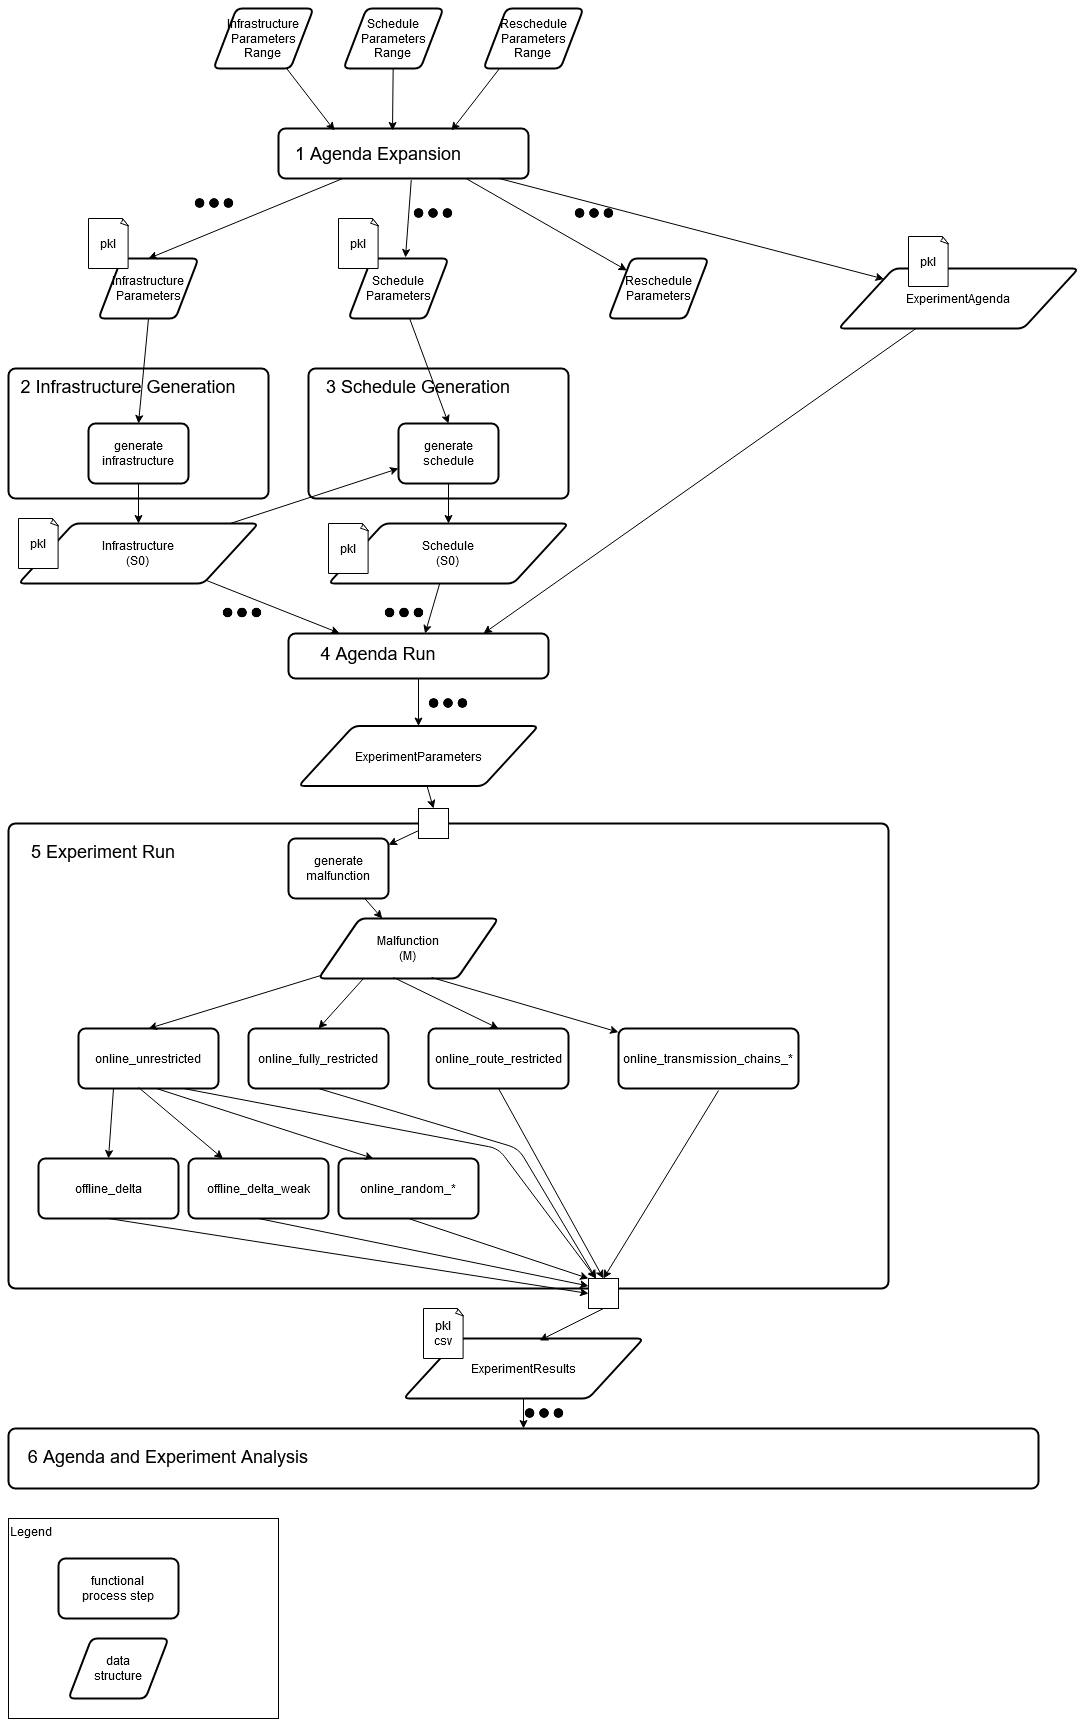
\includegraphics[width=0.8\textwidth]{Figures/03_pipeline/H1_overview.png}
	\caption{Pipeline for hypothesis H1 as functional diagram with intermediate data structures at two levels. The top level consists of four stages.}
	\label{fig:H1_overview}
\end{figure}
%
the pipeline decomposes into five top-level stages:
\begin{description}[%
  before={\setcounter{descriptcount}{0}},%
  ,font=\bfseries\stepcounter{descriptcount}\thedescriptcount~]
\item[Infrastructure Generation] This generates railway topologies and places agent start and targets in the infrastructure. We will cover this stage in detail in Section~\ref{subsubsec:infrastructuregeneration}\footnote{Conceptually, the placement of agents should be separated from infrastructure generation. However, the way FLATland is designed, it is not possible without refactoring to separate the two as the information about cities/stations is only available during infrastructure generation and agent placement.}
\item[Schedule Generation] This generates the exact conflict-free paths and times through the infrastructure for all agents. We will cover this stage in detail in Section~\ref{subsubsec:schedulegeneration}.
\item[Malfunction Generation] We define the type and time of the malfunction. Throughout this research project we use single train time delay as malfunction, i.e. Agents gets halted for $x$ timesteps during simulation. See Section~\ref{subsubsec:malfunctiongeneration}.
\item[Experiment Run] Here, the different scopers are run on the same problem instance. We will cover these data structures and functional process steps in Sections~\ref{subsubsec:scheduleproblemdescription} and \ref{subsec:scopers}.
\item[Experiment Analysis] This stage aggregates the data and generates the plots that help to verify hypothesis H1 and H2 baseline. We will give more details in Sections~\ref{sec:Results} and \ref{sec:CaseStudies}.
\end{description}
Since the schedule generation step takes too long to repeat for every experiment, we will use the same infrastructure and schedule for many malfunctions. In fact, we can pre-generate infrastructures and schedules and then work on variations of the re-scheduling part of the pipeline more efficiently. We refer to \url{https://github.com/SchweizerischeBundesbahnen/rsp/blob/master/README.md} for practical getting started.



%%%%%%%%%%%%%%%%%%%%%%%%%%%%%%%%%%%%%%%%%%%%%%%%%%%%%%%%%%%%%%%%%%%%%%%%%%
\subsection{Infrastructure Generation}\label{subsubsec:infrastructuregeneration}
%%%%%%%%%%%%%%%%%%%%%%%%%%%%%%%%%%%%%%%%%%%%%%%%%%%%%%%%%%%%%%%%%%%%%%%%%%

The infrastructure consists of a grid of cells. Each cell consists of a distinct tile type which defines the movement possibilities of the agent through the cell. There are 8 basic tile types, which describe a rail network. For each direction a train can pass through a cell, there are at most two options available, there are no 3-way forks.
%
Figure~\ref{fig:H1_railway_elements} shows eight basic cell types of a FLATland grid (top) and their translation into a directed graph (bottom).
%
\begin{figure}[hbtp]
	\centering
  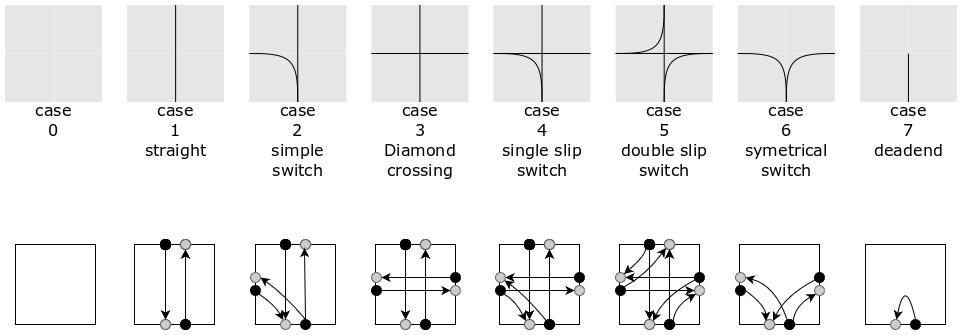
\includegraphics[width=0.8\textwidth]{Figures/03_pipeline/H1_railway_elements.png}
	\caption{Overview of the eight basic types in the top row. These basic types can be rotated in steps of $45^\circ$ and mirrored along the North--South or East--West axis to give all possible cell types. The bottom row shows the corresponding translation into a graph structure: squares represent cells, black dots represent an entry pin into the depicted cell and a grey dot represents the pin in the opposite direction into the neighboring cell.}
	\label{fig:H1_railway_elements}
\end{figure}
%
The result of this translation is captured formally as \emph{railway infrastructure}, which define to be a tuple  $(\mathcal{C}, \mathcal{V}, \mathpzc{c}, \mathcal{E})$, where
\begin{itemize}
    \item $\mathcal{C}$ is a set of cells,
    \item $\mathcal{V}$ is the set of pins by which the cell can be entered (they are positioned to the north, east, south or east of the cell),
    \item $\mathpzc{c}: \mathcal{V} \to \mathcal{C}$ which associates to each ``pin'' the cell it enters (there are at most $4$ pins for every cell),
    \item $\mathcal{E} \subseteq \mathcal{V} \times \mathcal{V}$, the possible directed transitions in the grid;
    \item $(\mathcal{V},\mathcal{E})$ is an acyclic graph.
\end{itemize}
Intuitively, we have a directed graph of routing possibilities where in addition each edge (identified by its entering node) is related to a cell (or more generally a resource) that it occupies.

To generate the infrastructure for our experiments we utilize the \textit{sparse\_rail\_generator} which is part of the FLATland environment. It uses the following parameters to generate a railway infrastructure.

 \begin{itemize}
    \item \textbf{number\_of\_agents:} The number of trains in the schedule
    \item \textbf{width:} Number of cells in the width of the environment
    \item \textbf{height:} Number of cells in the height of the environment
    \item \textbf{flatland\_seed\_value:} Random seed to generate different configurations
    \item \textbf{max\_num\_cities:} Maximum number of cities to be places in the environment. Cities are the only places where agents can start or end their journey. Cities consists of parallel track and entry/exit ports.
    \item \textbf{max\_rail\_in\_city:} Maximum number of parallel tracks in the city
    \item \textbf{max\_rail\_between\_cities:} Maximum number of parallel track at entry/exit ports of the cities
 \end{itemize}

The generated cities are illustrated in figure \ref{fig:city_structure}, which in turn are connected together to form a closed infrastructure system as shown in figure \ref{fig:flatland_map}.

\begin{figure}[hbtp]
	\centering
  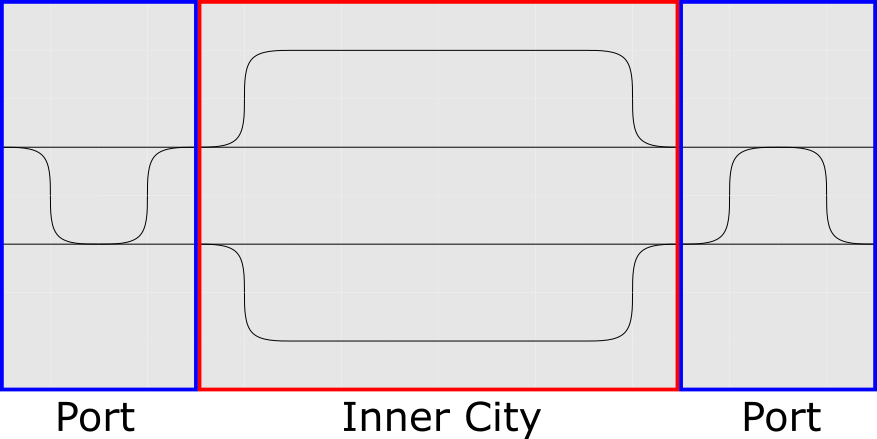
\includegraphics[width=0.75\textwidth]{Figures/city_structure.png}
	\caption{Example of a generated city in flatland. The parallel tracks are used as starting or target points for the agents. Ports connect to neighbouring cities through long rail tracks.}
	\label{fig:city_structure}
\end{figure}



\begin{figure}[hbtp]
	\centering
  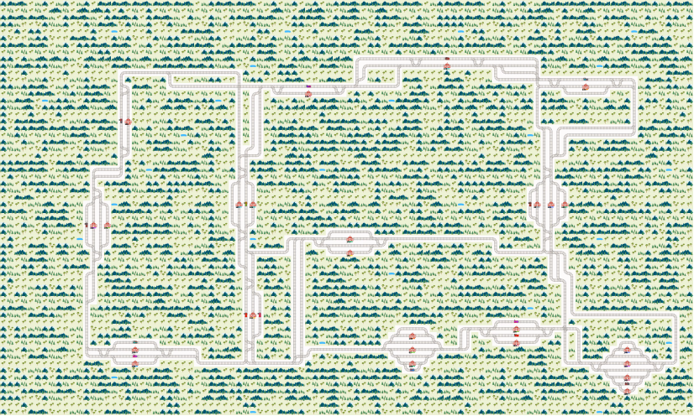
\includegraphics[width=\textwidth]{Figures/flatland_map.png}
	\caption{Example infrastructure generated by \textit{sparse\_rail\_generator}. The cities vary with number of parallel tracks as specified in the generator parameters. The complexity of the infrastructure can be enhances by reducing the number of available tracks within and between cities.}
	\label{fig:flatland_map}
\end{figure}


%%%%%%%%%%%%%%%%%%%%%%%%%%%%%%%%%%%%%%%%%%%%%%%%%%%%%%%%%%%%%%%%%%%%%%%%%%
\subsection{General Train Scheduling Problem}\label{subsubsec:scheduleproblemdescription}
%%%%%%%%%%%%%%%%%%%%%%%%%%%%%%%%%%%%%%%%%%%%%%%%%%%%%%%%%%%%%%%%%%%%%%%%%%



We introduce the abstract model from \cite{DBLP:journals/corr/abs-2003-08598}, which we use both for schedule generation and for re-scheduling; we could use any schedule as input, but we use the same solver model for practical reasons; the difference between these two applications is only in the optimization objective used as detailed in Sections~\ref{subsubsec:schedulegeneration} and \ref{subec:objectiveresched}, respectively, as well as different search heuristics in the solver.
Furthermore, the model introduced in this section is more general than we actually need for our experiments for H1; this will allow us to review the synthetic assumptions of Section~\ref{subsec:playground} in a more formal setting.


According to \cite{DBLP:journals/corr/abs-2003-08598},  the \emph{(general) train scheduling problem} is formalized as a tuple $(N, \mathcal{A}, C, F)$ having the following components
\begin{itemize}
    \item $N$ stands for the railway network $(V, E, R, m, a, b)$, where
        \begin{itemize}
            \item $(V, E)$ is a directed graph,
            \item $R$ is a set of resources,
            \item $m:E\to\mathbb{N}$ assigns the minimum travel time of an edge,
            \item $a: R\to 2^E$ associates resources with edges in the railway network, and
            \item $b:R\to \mathbb{N}$ gives the time a resource is blocked after it was accessed by a train line.
        \end{itemize}
    \item $\mathcal{A}$ is an indexed set of train lines to be scheduled on network $N$. Each train $\mathcal{A}(a)$ for agent id $a\in \dom(\mathcal{A})$ is represented as a tuple $\mathcal{A}(a)=(S, L, e, l, w)$, where
        \begin{itemize}
            \item $(S, L)$ is an acyclic subgraph of $(V, E)$,
            \item $e:S \to \mathbb{N}$ gives the earliest time a train may arrive at a node,
            \item $l:S\to \mathbb{N} \cup \left\{\infty\right\}$ gives the latest time a train may arrive at a node, and
            \item $w:L\to \mathbb{N}$ is the time a train has to wait on an edge.
        \end{itemize}
        Note that all functions are total unless specified otherwise.
        \item $C$ contains connections requiring that a certain train line $a^\prime$ must not arrive at node $n^\prime$ before another train line $a $ has arrived at node $n$ for at least $\alpha$ and at most $\omega$ discrete time steps. More precisely, each connection in $C$ is of form $(t,(v, v^\prime), t^\prime,(u, u^\prime), \alpha, \omega, n, n^\prime)$ such that $a= (S, L, e, l, w)\in \mathcal{A}$ and $a^\prime= (S^\prime, L^\prime, e^\prime, l^\prime, w^\prime)\in \mathcal{A}$, $a\not=a^\prime$,$(v, v^\prime)\in L$,$(u, u^\prime)\in L^\prime$,$\left\{\alpha,\omega\right\} \subseteq \mathbb{Z} \cup \left\{\infty,-\infty\right\}$, and either $n=v$ or $n=v^\prime$, as well as, either $n^\prime=u$ or $n^\prime=u^\prime$.
    \item Finally, $F$ contains collision-free resource points for each connection in $C$. We represent it as a family $(F_c)_{c\in C}$. Connections removing collision detection are used to model splitting (or merging) of trains, as well as reusing the whole physical train between two train lines. More importantly, this allows us to alleviate the restriction that subgraphs for train lines are acyclic, as we can use two train lines forming a cycle that are connected via such connections.
\end{itemize}
We refer to \cite{DBLP:journals/corr/abs-2003-08598} for more details.
In this setting, edges can be interpreted as time slices of a train run referring to a certain speed profile since the resources to be reserved ahead may depend on the speed profile; however, the model has no reference to the underlying geography (coordinates etc.); also, resources are abstract, there is no notion of location in general -- resources might represent track sections that need to be reserved, but they may also be gates or sideway tracks or signals that need to be reserved while travelling the edge. Notice that different trains may have the same edges in their route DAG (directed acyclic graph), which means that they can drive with the same speed profile at the same place.





We now define solutions: the \emph{solution to a train scheduling problem} $(N, \mathcal{A}, C, F)$ is a pair $(P,A)$ consisting of
\begin{enumerate}
    \item a function $P$ assigning to each train line the path it takes through the network, and
    \item an assignment $A$ of arrival times to each train line at each node on their path.
\end{enumerate}
A path is a sequence of nodes, pair-wise connected by edges. We write $v\in p$ and $(v, v^\prime)\in p$ to denote that node $v$ or edge $(v, v^\prime)$ are contained in path $p=(v_1, . . . , v_n)$, that is, whenever $v=v_i$ for some $1\leq i \leq n$, or this and additionally $v^\prime=v_{i+1}$, respectively.
%
A path $P(a) = (v_1, . . . , v_n)$ for $a= (S, L, e, l, w)\in \mathcal{A}$ has to satisfy
\begin{equation}
v_i \in S \textrm{ for }1\leq i \leq n \label{eq:ASP_1},
\end{equation}
\begin{equation}
(v_j, v_{j+1})\in L \textrm{ for } 1\leq j \leq n-1 \label{eq:ASP_2}
\end{equation}
\begin{equation}
in(v_1) = 0 \textrm{ and } out(v_n) = 0,\label{eq:ASP_3}
\end{equation}
where $in$ and $out$ give the in- and out-degree of a node in graph $(S, L)$, respectively.
We will write $\tau(a,P)=v_n$ for the target node used by agent $a$ in the schedule $(P,A)$, and, similarly $\sigma(a,P)=v_1$ for the source node of agent $a$ in the schedule $(P,A)$.
Intuitively, Conditions (\ref{eq:ASP_1}) and (\ref{eq:ASP_2}) enforce paths to be connected and feasible for the train line in question and Condition (\ref{eq:ASP_3}) ensures that each path is between a possible start and end node.
An assignment $A$ is a partial function $\mathcal{A}\times V\to \mathbf{N}$, where $A(a, v)$ is undefined whenever$v\not\in P(a)$. In addition, given path function $P$, an assignment $A$ has to satisfy the conditions in (\ref{eq:ASP_4}) to (\ref{eq:ASP_8}):
\begin{equation}
A(a, v_i)\geq e(v_i)\label{eq:ASP_4}
\end{equation}
\begin{equation}
A(a, v_i)\leq l(v_i)\label{eq:ASP_5}
\end{equation}
\begin{equation}
A(a, v_j) +m((v_j, v_{j+1})) +w((v_j, v_{j+1}))\leq A(a, v_{j+1})\label{eq:ASP_6}
\end{equation}
for all $a= (S, L, e, l, w)\in\mathcal{A}$ and $P(a) = (v_1, . . . , v_n)$ such that $1\leq i\leq n$,$1\leq j\leq n-1$,
either
\begin{equation}
A(a, v^\prime) +b(r) \leq A(a^\prime, u) \textrm{ or }A(a^\prime, u^\prime) +b(r)\leq A(a, v) \label{eq:ASP_7}
\end{equation}
for all $r\in R$, ${a, a^\prime} \subseteq \mathcal{A}$, $a\not=a'$,$(v, v^\prime)\in P(a)$,$(u, u^\prime)\in P(a^\prime)$ with $\left\{(v, v^\prime),(u, u^\prime)\right\} \subseteq a(r)$ whenever for all $(a,(x, x^\prime), a^\prime,(y, y^\prime), \alpha, \omega, n, n^\prime)\in C$ such that $(x, x^\prime)\in P(a)$,$(y, y^\prime)\in P(a^\prime)$, we have $(a,(v, v^\prime), a^\prime,(u, u^\prime), r)\not\in F_c$, and finally
\begin{equation}
\alpha\leq A(t^\prime, n^\prime)-A(t, n)\leq \omega\label{eq:ASP_8}
\end{equation}
for all $(a,(v, v^\prime), a^\prime,(u, u^\prime), \alpha, \omega, n, n^\prime)\in C$ if $(v, v^\prime)\in P(a)$ and $(u, u^\prime)\in P(a^\prime)$.
%
Intuitively, conditions (\ref{eq:ASP_4}), (\ref{eq:ASP_5}) and (\ref{eq:ASP_6}) ensure that a train line arrives at nodes neither too early nor too late and that waiting and traveling times are accounted for. Furthermore, Condition (\ref{eq:ASP_7}) resolves conflicts between two train lines that travel edges sharing a resource, so that one train line can only enter after another has left for a specified time span. This condition does not have to hold if the two trains use a connection that defines a collision-free resource point for the given edges and resource. Finally, Condition (\ref{eq:ASP_8}) ensures that train line $a$ connects to $a^\prime$ at node $n$ and $n^\prime$, respectively, within a time interval from $\alpha$ to $\omega$. Note that this is only required if both train lines use the specific edges specified in the connections. Furthermore, note that it is feasible that $n$ and $n^\prime$ are visited but no connection is required since one or both train lines took alternative routes.





%%%%%%%%%%%%%%%%%%%%%%%%%%%%%%%%%%%%%%%%%%%%%%%%%%%%%%%%%%%%%%%%%%%%%%%%%%
\subsection{Schedule Generation}\label{subsubsec:schedulegeneration}
%%%%%%%%%%%%%%%%%%%%%%%%%%%%%%%%%%%%%%%%%%%%%%%%%%%%%%%%%%%%%%%%%%%%%%%%%%



We start schedule generation from  infrastructure generation as described in Section~\ref{subsubsec:infrastructuregeneration}; correctly, we should have introduced an additional layer into our hierarchical approach, splitting our infrastructure generation into infrastructure and service intention; for purely practical reasons only did we refrain from doing this (FLATland does not store the station areas in the final layout, they are only temporary data structures during grid generation, and we would have had to extend FLATland for this purpose). We start schedule generation from the following elements:
\begin{itemize}
    \item railway infrastructure $(\mathcal{C}, \mathcal{V}, \mathpzc{c}, \mathcal{E}$
    \item $\mathcal{A}$ of trains or agents;
    \begin{itemize}
        \item each train $a\in \dom\mathcal{A}$ has a source $\sigma(a)\in\mathcal{V}$ and some target in $\tau(a)\subseteq\mathcal{V}$\footnote{The asymmetry comes from FLATland where we always start in a cell with a direction; however the target cell may be reached by any direction.}
        \item a speed $v(a) \in [0,1]$
        \item a path restriction represented by acyclic subgraph $(\mathcal{V}_a,\mathcal{E}_a)$
    \end{itemize}

    \item a release time $r$\footnote{Technically, we need a release time $r>0$ if we want to be able to replay solutions in FLATland, which allows the next agent (in the order of agent indices) to enter a grid cell; with $r>0$ we can force agents to stop and control by actions which agent will be the next to enter the cell.}, which specifies how long a cell remains blocked after a train has left it and which we assume the same for all resources in our setting.
\end{itemize}
In summary, we have $\mathcal{C}, \mathcal{V}, \mathpzc{c}, \mathcal{E}, \mathcal{A},\sigma,\tau,v,r,\Set{(\mathcal{V}_a,\mathcal{E}_a)}_{a \in \mathcal{A}}$.
We now show how a general train scheduling problem $(N,\tilde{\mathcal{A}},C,F)$ can be derived:
\begin{itemize}
    \item $\tilde{\mathcal{A}}$ consists of a tuple $(S,L,e,l,w)$ for each $a \in \mathcal{A}$ where
        \begin{itemize}
            \item $S=\mathcal{V}_a$
            \item $L=\mathcal{E}_a$
            \item $e(v)=\min_{p: \sigma(a)\textrm{--}v\textrm{ path in }(\mathcal{V}_a,\mathcal{E}_a)} \left|p\right| \cdot {v(a)}^{-1}$
            \item $l(v)=\max_{p: v\textrm{--}\tau(a)\textrm{ path in }(\mathcal{V}_a,\mathcal{E}_a)} U-\left|p\right| \cdot {v(a)}^{-1}$
            \item $w(e)={v(a)}^{-1}$\mbox{  }\footnote{This does not respect the intended semantics of the general model. Therefore, it would be better to use $S=\{ (v,{v(a)}^{-1}): v \in P_a\}$, $L=\{ ((v_1,{v(a)}^{-1}),(v_2,{v(a)}^{-1})): (v_1,v_2) \in P_a\}$, $w(e)=0$ and $m(((v_1,{v(a)}^{-1}),(v_2,{v(a)}^{-1})))={v(a)}^{-1}$, reflecting the idea that the routing graph represents speed profiles.};
        \end{itemize}
        \item $N=(V,E,R,m,a,b)$ where
        \begin{itemize}
            \item $V=\bigcup_{a \in \mathcal{A}} V_a$
            \item $E=\bigcup_{a \in \mathcal{A}} E_a$
            \item $R=\mathcal{C}$
            \item $m(e)=0$, $e \in E$
            \item $a(c) = \left\{ e=(v_1,v_2): \mathpzc{c}(v_1)=c \right\}$, $c\in R$
            \item $b(c)=r$, $c\in R$;
        \end{itemize}
    \item $C=\emptyset$;
    \item $F=\emptyset$.
\end{itemize}
Some remarks on this transformation:
\begin{itemize}
    \item In our setting, we only have one resource per edge, i.e. we only reserve the train's own track, per cell. There is a $n:1$ correspondence between edges and resources. In general, the correspondence can be $n:m$ (a train may reserve path ahead or signals along its position depending on its speed)
    \item The earliest and latest windows are designed such that they represent the earliest possible time the train can reach the vertex, respectively, the latest possible time the train must pass in order to be able to reach the target within the time limit.
    \item In our setting, $b$ is the same for all resources.
    \item In our setting, the minimum running per cell (by abuse, $w(e)= {v(a)}^{-1}$  for all $e \in L$ for all agents $a \in \dom(\mathcal{A})$)
    \item In our setting, we do not have intermediate stops (by abuse, $m(e)=0$ for all $e \in E$)
    \item In our setting, there are no connections nor collision-free resources.
\end{itemize}

The time windows given by $e$ and $l$ can be computed by Algorithm~\ref{algo:propagate_earliest} and \ref{algo:propagate_latest}, respectively. They propagate the minimum running time forward from an initial set of earliest and backwards from an initial set of latest constraints. An illustration can be found in Figures~\ref{fig:propagate_earliest} and \ref{fig:propagate_latest}, respectively.
The time windows are thus given by
$$e\leftarrow propagate\_earliest(\Set*{e(\sigma(a))=0}, (S,L), \Set*{\sigma(a)}, {v(a)}^{-1})$$ and $$l\leftarrow propagate\_latest(\Set*{e(\tau)=U: \tau \in S, out(\tau)=0}, (S,L), \Set*{\tau \in S: out(\tau)=0},{v(a)}^{-1}).$$
Finally, we can remove nodes $v$ with empty time window $e(v)>l(v)$.





\begin{algorithm}
	\caption{$propagate\_earliest$} \label{algo:propagate_earliest}
	\begin{algorithmic}[1]
	    \Require $e$, $(S,L)$, $F$, $mrt$ s.t. $F\subseteq \dom(e)$
	    \Ensure $e$
	    \State $Open \leftarrow F$
	    \For {$v \in Open$}
    	    \For {$v^\prime \in S-F: (v,v^\prime) \in L$}
    	        \If{$v^\prime \not\in \dom(e)$}
    	            \State $e(v^\prime) \leftarrow \infty$
    	        \EndIf
    			\State $e(v) \leftarrow \min \Set*{e(v^\prime), e(v)+mrt}$
    			\State $Open \leftarrow Open \cup \Set*{v^\prime}$
    		\EndFor
			\State $Open \leftarrow Open - \Set*{v}$
		\EndFor
	\end{algorithmic}
\end{algorithm}

\begin{figure}[hbtp]
	\centering
  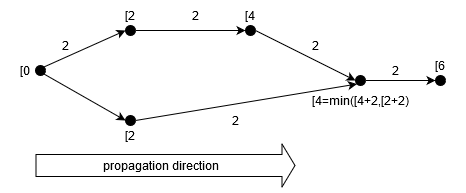
\includegraphics[width=0.8\textwidth]{Figures/03_pipeline/H1_propagate_earliest.png}
	\caption{Illustration of $propagate\_earliest$ for an agent $a$ with speed $v(a)=\frac{1}{2}$ (i.e. $mrt=2$).}
	\label{fig:propagate_earliest}
\end{figure}


\begin{algorithm}
	\caption{$propagate\_latest$} \label{algo:propagate_latest}
	\begin{algorithmic}[1]
	    \Require $l$, $(S,L)$, $F$, $mrt$  s.t. $F\subseteq \dom(l)$
	    \Ensure $l$
	    \State $Open \leftarrow F$
	    \For {$v \in Open$}
    	    \For {$v^\prime \in S-F: (v^\prime,v) \in L$}
    	        \If{$v^\prime \not\in \dom(l)$}
    	            \State $l(v^\prime) \leftarrow -\infty$
    	        \EndIf
    			\State $l(v) \leftarrow \max \Set*{l(v^\prime), l(v)-mrt}$
    			\State $Open \leftarrow Open \cup \Set*{v^\prime}$
    		\EndFor
			\State $Open \leftarrow Open - \Set*{v}$
		\EndFor
	\end{algorithmic}
\end{algorithm}


\begin{figure}[hbtp]
	\centering
  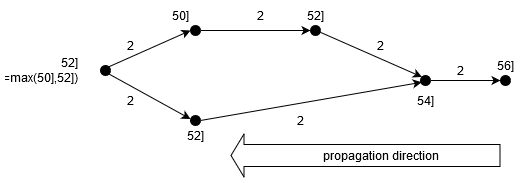
\includegraphics[width=0.8\textwidth]{Figures/03_pipeline/H1_propagate_latest.png}
	\caption{Illustration of $propagate\_latest$ for an agent $a$ with speed $v(a)=\frac{1}{2}$ (i.e. $mrt=2$) and for upper bound $U=56$.}
	\label{fig:propagate_latest}
\end{figure}



For schedule generation, we use a different objective function than for re-scheduling, namely minimizing
\begin{equation}
\sum_{a \in \mathcal{A}, v,v^\prime \in P(a), in(v)=0, out(v^\prime)=0} A(a,v^\prime) - A(a,v)
\end{equation}
and restricting
\begin{equation}
\max_{a \in \mathcal{A}, v \in P(a)} A(a,v) \leq U,
\end{equation}
where we use the following heuristic for the upper bound,
\begin{equation}
U=\alpha \cdot \delta \cdot  \left(w + h + \frac{\left|\mathcal{A}\right|}{\left| S \right|} \right)
\end{equation}
and $\alpha=2$ and $\delta=4$,
to find a schedule $S$ for a given service intention. This objective function is intended to mimick a green wave behaviour of real-world train scheduling (schedules are constructed such that there are only planned stops for passenger boarding and alighting); however, this also keeps us from introducing time reserves in the schedule and trains will not be able to catch up in our synthetic world once a delay has occured.


The choice of $U$ represents a worst case:
$w+h$ is an approximation of the longest possible path, $\frac{\left|\mathcal{A}\right|}{\left| S \right|}$ is the expected number of agents per city, hence the sum represents the time required for the last agent at the station if they all start one after the other and have constant speed; $\delta$ represents the minimum time required per cell for an agent running at minimum speed level $\frac{1}{4}$ (we use 4 levels $\frac{1}{i}$, $i=1,\ldots,4$) and $\alpha$ is a tolerance term that should allow for feasibility (there is no guarantee though).


Furthermore, we only use the shortest path for each agent for scheduling in order to speed-up schedule generation; if the upper bound $U$ is chosen liberal enough, then a solution is found where no train stops during its run.


Notice that trains have no length in the model: an edge is exited when the next edge is entered, but remains blocked for $r$ time steps after exit. Train extension can be introduced into this model by requiring consecutive edges to require the same resource; this again highlights that edges in the general train scheduling problem do not represent physical track sections; physical track sections have to be represented by abstract resources.




%%%%%%%%%%%%%%%%%%%%%%%%%%%%%%%%%%%%%%%%%%%%%%%%%%%%%%%%%%%%%%%%%%%%%%%%%%
\subsection{Malfunction Generation}\label{subsubsec:malfunctiongeneration}
%%%%%%%%%%%%%%%%%%%%%%%%%%%%%%%%%%%%%%%%%%%%%%%%%%%%%%%%%%%%%%%%%%%%%%%%%%

Our experiment parameters contain the following parameters for malfunction generation:
\begin{itemize}
    \item $m_{earliest} \in \mathbb{N}$: the earliest time step the malfunction can happen after the scheduled departure;
    \item $m_{duration} \in \mathbb{N}$: how many time steps the train will be delayed;
    \item $m_{agent} \in \dom(\mathcal{A})$: the id of the train that is concerned.
\end{itemize}

Given the schedule, we derive our malfunction $M=(m_{time\_step},m_{duration},m_{agent})$ where
\begin{equation*}
m_{time\_step} = \min \left\{  A(m_{agent},\sigma(a, P)) + m_{earliest},  A(m_{agent},\tau(a,P) \right\},
\end{equation*}
which ensures that the agent malfunction happens while the train is running.




%%%%%%%%%%%%%%%%%%%%%%%%%%%%%%%%%%%%%%%%%%%%%%%%%%%%%%%%%%%%%%%%%%%%%%%%%%
\subsection{Objective for Re-Scheduling}\label{subec:objectiveresched}
%%%%%%%%%%%%%%%%%%%%%%%%%%%%%%%%%%%%%%%%%%%%%%%%%%%%%%%%%%%%%%%%%%%%%%%%%%

We chose to minimize a linear combination of delay with respect to the initial schedule $S_0$ and penalizing diverging route segments (only the first edge of each such segment). This reflects the idea of not re-routing trains without the need of avoiding delay; if re-scheduling is applied in an iterative loop, this should help to avoid ``flickering'' of decisions.
%
Formally, the objective is to minimize over solutions $S=(P_S,A_S)$  the sum
\begin{equation}
\sum_{a \in \mathcal{A}} \delta\left(S(a,\tau(a,S)) - S_0(a,\tau(a, S_0))\right) + \rho \cdot \left|\left\{v \in \mathcal{V}(S,a)-\mathcal{V}(S_0,a): (v^\prime,v) \in P_{S_0}(a) \right\}\right| \label{eq:objectiveresched}
\end{equation}
where the \emph{delay model} is step-wise linear,
\begin{equation}
\delta(t) =
\begin{cases}
    \infty & \textrm{ if } t \geq \delta_{cutoff},\\
    \floor{t / \delta_{step}} \cdot \delta_{penalty}  & \textrm{else},
\end{cases}
\end{equation}
for hyper-parameters $\delta_{step}$, $\delta_{cutoff}, \delta_{penalty}$
and the second term of (\ref{eq:objectiveresched}) penalizes re-routing with respect to the initial schedule $S_0$ by weight $\rho$ for every first edge deviating from the original schedule $S_0$ .


%%%%%%%%%%%%%%%%%%%%%%%%%%%%%%%%%%%%%%%%%%%%%%%%%%%%%%%%%%%%%%%%%%%%%%%%%%
\subsection{Re-Scheduling Scopes}\label{subsec:scopers}
%%%%%%%%%%%%%%%%%%%%%%%%%%%%%%%%%%%%%%%%%%%%%%%%%%%%%%%%%%%%%%%%%%%%%%%%%%

We now look at the different scopes of Section~\ref{subec:online_offline} in more detail. All these scopers have the same interface, i.e. take the same parameters:
\begin{itemize}
    \item an indexed set $\mathcal{A}$ of agents $\mathcal{A}(a)=(S,L,e,l,w)$ that needs to be restricted; in our setup, $S,L$ will contain more routing alternatives than in the scheduling problem $\bar{\mathcal{A}}$, but $e,v,w$ will be defined just the same as in $\bar{\mathcal{A}}$
    \item initial schedule $(P_{S_0},A_{S_0})$
    \item malfunction $M=(m_{time\_step},m_{duration},m_{agent})$;
    \item agent speeds $v(a)$, $a \in \dom(\mathcal{A})$
    \item maximum time window size $c$: this is the maximum time window in the re-scheduling problem
    \item upper bound $U$: we will increase the upper bound from scheduling by $m_{duration}$, which will ensure feasibility of the re-scheduling problem, as we will discuss below.
    \item offline scopers will also receive the full re-schedule solution $(P_S,A_S)$
\end{itemize}


The result of the scoper will be a modification of $\mathcal{A}$;
in the pseudo-code for the different scopers, we will not show $w$, which is constant $w(e)= {v(a)}^{-1}$ for all $e \in L$. The railway network  $N=(V,E,R,m,a,b)$ of the re-scheduling problem will be composed of the union of all these agents,
\begin{equation}
V=\bigcup_{(S,L,e,l,w)=\mathcal{A}(a), a \in \dom(\mathcal{A}}S, E=\bigcup_{(S,L,e,l,w)=\mathcal{A}(a), a \in \dom(\mathcal{A}}L,
\end{equation}
and $m,a,b$ the restrictions to $E$ and used resources by $E$.


In our setting, each edge has exactly one resource; therefore, each vertex points at exactly one resource. Hence, the following definition is sound:
\begin{equation}
    R(v) = r \textrm{ s.t. } (v,v^\prime) \in a(r)
\end{equation}


\begin{mdframed}
{\bf Christian} is there something missing here?
\end{mdframed}

%%%%%%%%%%%%%%%%%%%%%%%%%%%%%%%%%%%%%%%%%%%%%%%%%%%%%%%%%%%%%%%%%%%%%%%%%%
\subsubsection{Scoping Re-scheduling (online\_unrestricted)} \label{subsubsec:scope_online_unrestricted}
%%%%%%%%%%%%%%%%%%%%%%%%%%%%%%%%%%%%%%%%%%%%%%%%%%%%%%%%%%%%%%%%%%%%%%%%%%

We first describe the online\_unrestricted scope, which does not restrict the problem scope, as a general train scheduling problem. Let $N=(V,E,R,m,a,b)$ be the network of the train scheduling problem, $S_0=(P,A)$ be a solution to it and let $M=(m_{time\_step},m_{duration},m_{agent})$ be a malfunction.

For each train the $scoper\_online\_unrestricted$ reduces the problem scope through Algorithm~\ref{algo:Delta0}:
If the train is already done at the malfunction time step (line 1), it can be removed from the problem (line 2);
if the train has not started yet at the malfunction time step (line 3), we keep its start node fixed from $S_0$ and do not start earlier than in $S_0$ and use $propagate$ (described below) to derive the constraints (lines 4--11); in this case, the malfunction has no direct impact on the train and we do not allow the train to start earlier than scheduled.






\begin{algorithm}
	\caption{$scoper\_online\_unrestricted$ for train $a \in \dom(\mathcal{A})$} \label{algo:Delta0}
	\begin{algorithmic}[1]
		\Require $(S,L)$, $(P,A)$, $M=(m_{time\_step},m_{duration},m_{agent})$, mrt, U, c
	    \Ensure $(S,L),e,l$
        \If{$\max_{v\in S} A(v) \leq m_{time\_step}$}
            \State $S\leftarrow \emptyset$, $L \leftarrow \emptyset$
        \ElsIf{$\min_{v\in S} A(v) > m_{time\_step}$}
            \State $v_1 \leftarrow \argmin_{v\in S} A(v)$
            \State $e(v_1) \leftarrow A(v_1)$
            \For{$\tau \in S: out(\tau)=0$}
                \State $l(\tau)=U$
            \EndFor
            \State $F_v \leftarrow F_e \leftarrow \Set*{v_1}$
            \State $F_l \leftarrow \Set*{\tau \in S: out(\tau)=0}$
            \State $e,l,(S,L) \leftarrow propagate(e,l,(S,L),F_e,F_l,F_v, mrt, U, c)$
        \Else
            \State $e,l,(S,L) \leftarrow scoper\_online\_unrestricted\_running((S,L), (P,A), M, mrt, U, c)$
        \EndIf
\end{algorithmic}
\end{algorithm}


Before describing the third case of the malfunction happening while the train is running (lines 12--13), we describe \emph{propagate} (Algorithm~\ref{algo:propagate}): we pass in an initial, incomplete set of earliest and latest constraints which we want to propagate in the graph $(S,L)$ with the given minimum running time $mrt$ and such that $e$ in the output reflects the earliest possible time an agent can reach the vertex and that  $l$ reflects the last possible time the agent must reach the vertex to be able to still find a path to the target. Furthermore, we want some initial values not to be modifiable ($F_e$ and $F_l$) and we want to ``force'' some vertices that need be visited ($F_v$). In \emph{propagate}, we first remove the nodes that cannot be reached given $F_v$ (lines 1--4); then, we propagate earliest and latest (lines 5--6) and truncate time windows to $c$ (lines 7--10); we need to propagate latest again since truncation might spoil the semantics of $l(v)$ being the latest possible passing time to reach the target in time (line 11). Finally, we remove nodes that are not reachable in time because of an empty time window (line 13). Notice that different vertices at the same resource may have different time windows $e,l$. Since in our simplified setting, we do not have intermediate stations, we do not require propagate to respect the schedule at intermediate stations, where we would not want trains to depart earlier than published to customers.

\begin{algorithm}
	\caption{$propagate$} \label{algo:propagate}
	\begin{algorithmic}[1]
	    \Require $e,l,(S,L),F_e,F_l,F_v,mrt,U,c$
	    \Ensure $e,l,(S,L)$
        \For{$v \in F_v$}
		    \State $S \leftarrow \Set{v^\prime \in S: \textrm{there is a }v\textrm{--}v^\prime\textrm{ path or a }v^\prime\textrm{--}v\textrm{ path in }L}$
		    \State $L \leftarrow \Set*{(v,v^\prime) \in L: v,v^\prime \in S}$
		\EndFor
	    \State $e \leftarrow propagate\_earliest(e, (S,L), F_e, mrt)$
		\State $l \leftarrow propagate\_latest(l,(S,L),F_l, mrt)$
		\If{$c < \infty$}
		\For{$v\in S-F_e$}
	        \State $l(v) \leftarrow \min \Set*{l(v), e(v)+c}$
	    \EndFor
	    \State $l \leftarrow propagate\_latest(l,(S,L),F_l, mrt)$
	    \EndIf
		\State $S \leftarrow \Set{v \in S: e(v) \leq l(v)}$, $L \leftarrow \Set*{(v,v^\prime) \in L: v,v^\prime \in S}$

	\end{algorithmic}
\end{algorithm}



We now describe the remaining case of Algorithm~\ref{algo:Delta0}, namely when the malfunction happens while the train is running. We refer to Algorithm~\ref{algo:scoper_online_unrestricted_running} for $scoper\_online\_unrestricted\_running$: we first determine the edge $(v_1,v_2)$ the train is on when the malfunction happens; we then fix the time for $v_1$ as in $S_0$ and set the earliest for $v_2$, possibly delayed. Then, we use $propagate$ to tighten the search space. Notice that $propagate$ will here remove the nodes on the scheduled path before $v_1$ (since the forward propagation will not reach these nodes, they will be removed as the time window will be empty in the spirit of option 1 described above).


\begin{algorithm}
	\caption{$scoper\_online\_unrestricted\_running$ for running train $a \in \dom(\mathcal{A})$} \label{algo:scoper_online_unrestricted_running}
	\begin{algorithmic}[1]
		\Require $(S,L)$, $(P,A)$, $M=(m_{time\_step},m_{duration},m_{agent})$, mrt, U, c
	    \Ensure $e,l,(S,L)$
	    \State $(v_1,v_2) \leftarrow (v_1,v_2) \in L$ s.t. $A(v_1)\leq m_{time\_step}$ and $A(v_2)>m_{time\_step}$
		\State $e(v_1)\leftarrow A(v_1)$, $l(v_1) \leftarrow A(v_1)$
        \If{$a = m_{agent}$}
            \State $e_1(v_2) \leftarrow A(v_1)+mrt+m_{duration}$
        \Else
            \State $e_1(v_2) \leftarrow A(v_1)+mrt$
        \EndIf
        \State $F_e \leftarrow \Set*{v_1,v_2}$, $F_l \leftarrow \Set*{v_1} \cup \Set*{\tau \in S: out(\tau)=0}$

	    \For{$\tau \in S-\Set*{v_1}: out(\tau)=0$}
	        \State $l(\tau) \leftarrow U$
	    \EndFor
		\State $e,l,(S,L) \leftarrow propagate(e,l,(S,L),F_e,F_l, \Set*{v_1,v_2}, mrt, U, c)$
	\end{algorithmic}
\end{algorithm}


Notice that this problem always has a trivial feasible solution where all agents stop and restart in synchronicity with the malfunction agent (as said above, we extend the upper bound from scheduling by the malfunction duration).


%%%%%%%%%%%%%%%%%%%%%%%%%%%%%%%%%%%%%%%%%%%%%%%%%%%%%%%%%%%%%%%%%%%%%%%%%%
\subsubsection{Trivial upper-bound scoping (offline\_fully\_restricted)}
\label{subsubsec:scope_fully_restricted}
%%%%%%%%%%%%%%%%%%%%%%%%%%%%%%%%%%%%%%%%%%%%%%%%%%%%%%%%%%%%%%%%%%%%%%%%%%

The scoper offline\_fully\_restricted of Algorithm~\ref{algo:scoper_offline_fully_restricted} takes a schedule as input and yields a scheduling problem which has exactly the same schedule as only solution. This allows to determine the solver overhead as a lower bound of re-scheduling computation time.



\begin{algorithm}
	\caption{$scoper\_offline\_fully\_restricted$ for  train $a \in \dom(\mathcal{A})$} \label{algo:scoper_offline_fully_restricted}
	\begin{algorithmic}[1]
		\Require $(S,L)$, $(P,A)$, $M=(m_{time\_step},m_{duration},m_{agent})$, $mrt$, $U$, $c$
	    \Ensure $e,l,(S,L)$
        \State $S \leftarrow \Set*{v: v\in P}$
        \State $L \leftarrow \Set*{(v,v^\prime) \in P: v,v^\prime \in S}$
        \State $e \leftarrow \Set*{(v,P(v): v\in S}$
        \State $l \leftarrow \Set*{(v,P(v): v\in S}$
	\end{algorithmic}
\end{algorithm}

%%%%%%%%%%%%%%%%%%%%%%%%%%%%%%%%%%%%%%%%%%%%%%%%%%%%%%%%%%%%%%%%%%%%%%%%%%
\subsubsection{``Perfect'' delta scoping (offline\_delta)}
\label{subsubsec:scope_offline_delta}
%%%%%%%%%%%%%%%%%%%%%%%%%%%%%%%%%%%%%%%%%%%%%%%%%%%%%%%%%%%%%%%%%%%%%%%%%%

The idea of the ``perfect'' scoping is to have a baseline where we extract as much information as possible from a pre-computed offline solution without giving the solution right away.
%
Formally, let $(P_{S_0},A_{S_0})$ be the solution to the original train scheduling problem
and let $N_S=(V_S,E_S,R_S,m_S,a_S,b_S)$ be the network of the re-scheduling problem for an agent
and  let $(P_S,A_S)$ be a solution to the re-scheduling problem. Algorithm~\ref{algo:scoper_offline_delta} defines the ``perfect'' problem scope for a running agent: by keeping all times and nodes that are common to $S_0$ and $S$ fixed, respectively (lines 1--10).
The vertex after the malfunction is delayed by the malfunction duration (lines 11--18).
Everything that is not reachable in path ($F=\Delta_P$) or time ($F_e=F_l=\Delta_A$) is removed by $propagate$ (line 19). Notice that we have $v_1 \in \Delta_A \subseteq \Delta_P$ and $v_2 \in \Delta_P$


\begin{algorithm}
	\caption{$scoper\_offline\_delta$ for running train $a \in \dom(\mathcal{A})$} \label{algo:scoper_offline_delta}
	\begin{algorithmic}[1]
		\Require $(S,L)$, $(P_{S_0},A_{S_0})$, $M=(m_{time\_step},m_{duration},m_{agent})$, mrt, U, c, $(P_S,A_S)$
	    \Ensure $e,l,(S_1,L_1)$
	    \State $\Delta_A \leftarrow \Set*{v: A_S(v)=A_{S_0}(v), v\in P_{S_0}, v \in P_S}$
	    \State $\Delta_P \leftarrow \Set*{v: v\in P_S, v\in P_{S_0}, v\in P_{S_0}, v \in P_S}$
	    \State $S_1 \leftarrow \Set*{v: v\in P_{S_0}} \cup \Set*{v: v\in P_{S}}$
	    \State $L_1 \leftarrow \Set*{(v,v^\prime) \in P_S \textrm{ or } (v,v^\prime) \in P_{S_0}: v,v^\prime \in S_1}$
	    \For {$v \in \Delta_A$}
	        \State $l(v)\leftarrow e(v)\leftarrow A_{S_0}(v)$
	    \EndFor
	    \For{$v \in S_1-\Delta_A: out(v)=0$}
	        \State $l(v) \leftarrow U$
	    \EndFor
	    \State $(v_1,v_2) \leftarrow (v_1,v_2) \in L_1$ s.t. $A_{S_0}(v_1)\leq m_{time\_step}$ and $A_{S_0}(v_2)>m_{time\_step}$
	    \If{$v_2 \not \in \Delta_A$}
        \If{$a = m_{agent}$}
            \State $e_1(v_2) \leftarrow A_{S_0}(v_1)+mrt+m_{duration}$
        \Else
            \State $e_1(v_2) \leftarrow A_{S_0}(v_1)+mrt$
        \EndIf
        \EndIf
	    \State $e,l,(S_1,L_1) \leftarrow propagate(e,l,(S_1,L_1),\Delta_A \cup \Set*{v_2}, \Delta_A, \Delta_P, mrt, U, c)$
	\end{algorithmic}
\end{algorithm}
The solution space of this scoping contains the full re-scheduling solution if $c >= m_{duration}$, so the optimizer will find the same solution up to equivalence modulo cost.



%%%%%%%%%%%%%%%%%%%%%%%%%%%%%%%%%%%%%%%%%%%%%%%%%%%%%%%%%%%%%%%%%%%%%%%%%%
\subsubsection{``Weak'' delta scoping (offline\_delta\_weak)}\label{subsubsec:offline_delta_weak}
%%%%%%%%%%%%%%%%%%%%%%%%%%%%%%%%%%%%%%%%%%%%%%%%%%%%%%%%%%%%%%%%%%%%%%%%%%


To investigate the potential of simple online scopers we define a "weaker" offline scoper, which defines the reduced problem scope a all vertices and passing times for all agent which have any difference between $S$ and $S_0$.
The procedure of this scoper is explained in Algorithm~\ref{algo:scoper_offline_delta_weak}. The scoper frees up all the variables of changed trains, i.e., if a train has some change somewhere, it is given full routing and time flexibility. In Algorithm~\ref{algo:scoper_offline_delta_weak}, the changed agents are determined (line 1) and then the scope is reduced by Algorithm~\ref{algo:scoper_changed}:
all agents predicted as changed will have full re-scheduling degrees of freedom (lines 2--3), all others will be ``freezed'' to the original schedule (lines 6--10) or only forced to re-use the same route (lines 4--5), depending on whether $time\_flexibility$ is enabled or not.

\begin{algorithm}
	\caption{$scoper\_offline\_delta\_weak$} \label{algo:scoper_offline_delta_weak}
	\begin{algorithmic}[1]
		\Require $\mathcal{A}$, $(P_{S_0},A_{S_0})$,$M=(m_{time\_step},m_{duration},m_{agent})$,$v$,$U$,$U$,$c$, $(P_S,A_S)$
	    \Ensure $\mathcal{A}$
	    \State $\mathcal{A}^* \leftarrow \Set{a\in \dom(\mathcal{A}):  P_{S_0} \not=P_{S} \textrm { or } A_{S_0}(a,\cdot) \not= A_{S}(a,\cdot)}$
	    \State $\mathcal{A}^* \leftarrow scoper\_changed(\mathcal{A},(P_{S_0},A_{S_0}),\mathcal{A}^*,time\_flexibility=\bot,v,U,c)$
	\end{algorithmic}
\end{algorithm}




\begin{algorithm}
	\caption{$scoper\_changed$} \label{algo:scoper_changed}
	\begin{algorithmic}[1]
		\Require $\mathcal{A}$, $(P,A)$, $\mathcal{A}^*\subseteq\dom(\mathcal{A})$, $time\_flexibility$, $M$, $v$, $U$, $c$
	    \Ensure $\mathcal{A}$
	    \For{$a \in \dom(\mathcal{A})$}
    	    \If {$a \in \mathcal{A}^*$}
    	        \State $e,l,S,L \leftarrow scoper\_online\_unrestricted((S,L), (P,A), M, v^{-1}(a), U, c)$
    	    \ElsIf{$time\_flexibility$}
    	        \State $e,l,S,L \leftarrow scoper\_online\_path\_restricted((S,L), (P,A), M, v^{-1}(a), U, c)$
    	    \Else
    	        \State $e,l,S,L \leftarrow scoper\_online\_fully\_restricted((S,L), (P,A), M, v^{-1}(a), U, c$
    	    \EndIf
    	    \For{$e \in L$}
    	        \State $w(e) \leftarrow v^{-1}$
    	    \EndFor
    	    \State $\mathcal{A}(a) \leftarrow (S,L,e,v,w)$
	    \EndFor
	\end{algorithmic}
\end{algorithm}

Again, the solution space of this scoping contains the full re-scheduling solution, so we will find the same or a cost-equivalent solution.


%%%%%%%%%%%%%%%%%%%%%%%%%%%%%%%%%%%%%%%%%%%%%%%%%%%%%%%%%%%%%%%%%%%%%%%%%%
\subsubsection{Route-restricted Re-scheduling (online\_route\_restricted)}
\label{subsubsec:scope_online_route_restricted}
%%%%%%%%%%%%%%%%%%%%%%%%%%%%%%%%%%%%%%%%%%%%%%%%%%%%%%%%%%%%%%%%%%%%%%%%%%


Algorithm~\ref{algo:scoper_online_route_restricted} scopes the re-scheduling problem to the routes of the schedule $S_0$, but allows time flexibility: after discarding all vertices and edges not on scheduled path (lines 1--2), \emph{propagate} makes the constraints consistent. If $c\geq m_{duration}$, the resulting re-scheduling problem is clearly feasible; however, we expect solution quality to deterioriate.

\begin{algorithm}
	\caption{$scoper\_online\_route\_restricted$ for running train $a \in \dom(\mathcal{A})$} \label{algo:scoper_online_route_restricted}
	\begin{algorithmic}[1]
		\Require $(S,L)$, $(P,A)$, $M=(m_{time\_step},m_{duration},m_{agent})$, $mrt$, $U$, $c$
	    \Ensure $e,l,(S,L)$
        \State $S \leftarrow \Set*{v: v\in P}$
        \State $L \leftarrow \Set*{(v,v^\prime) \in P: v,v^\prime \in S}$
        \State $e,l,(S,L) \leftarrow propagate(e,l,(S,L),\emptyset, \emptyset, \emptyset, mrt, U, c)$
	\end{algorithmic}
\end{algorithm}


%%%%%%%%%%%%%%%%%%%%%%%%%%%%%%%%%%%%%%%%%%%%%%%%%%%%%%%%%%%%%%%%%%%%%%%%%%
\subsubsection{Re-Scheduling with Transmission Chains\\ (online\_transmission\_chains\_fully\_restricted,\\online\_transmission\_chains\_route\_restricted)}
\label{subsubsec:scope_online_tranmission_chains}
%%%%%%%%%%%%%%%%%%%%%%%%%%%%%%%%%%%%%%%%%%%%%%%%%%%%%%%%%%%%%%%%%%%%%%%%%%

This is an implementation of a simple heuristic scope reducing algorithm. It can instantly reduce the scope of a re-scheduling problem by assuming that all trains stay on their planned path and by propagating the caused delay forward in time, passing it on to any scheduled train within a temporal distance smaller than the malfunction duration.
%
Let $S_0=(P,A)$ be a schedule and let $P(a) = (v_1,\ldots,v_n)$ the scheduled path for an agent $a$, then  the exit time of the edge after an entry vertex is
\begin{equation}
E(a,v_i) = A(a,v_{i+1}) + r
\end{equation}
for $i=1,\ldots,n-1$ and $E(a,v_n) = A(a,v_n)+r$.

Now we can have a look at Algorithm~\ref{algo:transmission_chains}: we have a queue $q$ where we store which agents are reached, at which vertex and how much of the delay is propagated (line 1). In order to prevent loops, we store the elements of the queue already dealt with (line 2).  The output will be a set of agents reached, initialized with the malfunction agent (line 3).
We initialize the queue and the changed agents with the malfunction agent by pushing all vertices that are passed in the schedule after the malfunction; since the schedule is constructed such that the agents never stop, the delay is not reduced (lines 4--6) \footnote{If there are time reserves in the schedule, the propagated delay could be compensated by consuming this time reserve. In our implementation, schedules have almost no }.
Then, we look at the next agent after the queued element (lines 8--14). If the delay cannot be absorbed by the time difference between the queued element's departure and the next agent entry (lines 16--17), then we mark the next agent as reached (line 18),
compute the transmitted delay (line 19).
If the there is a delay $d^\prime >0$ propagated to $a^\prime$, then $a^\prime$ cannot enter $R(v)$ only $d^\prime$ later, i.e. the occupation of the previous call $R(v^{\prime\prime})$ is prolonged by $d^\prime$, which may cause other agents to wait for $a^\prime$'s delayed departure. Finally, we  enqueue all vertices scheduled after it is ``hit`` by the propagated delay (lines 24--25), starting at the cell before $R(v)$.
As an illustration, take another agent is scheduled to go through the malfunctioning agent as it stands still but the other agent is not opened up and is forced to keep its schedule, then the problem is infeasible; there may be many more such situations by transitivity. The output of this prediction can then be passed to Algorithm~\ref{algo:scoper_changed} with or without time flexibility.






\begin{algorithm}
	\caption{$changed\_transmission\_chains$} \label{algo:transmission_chains}
	\begin{algorithmic}[1]
		\Require $\mathcal{A}$, $(P,A_{S_0})$, $M=(m_{time\_step},m_{duration},m_{agent})$
	    \Ensure $\mathcal{A}^* \subseteq \mathcal{A}$
	    \State $q = queue()$
	    \State $done = \emptyset$
	    \State $\mathcal{A}^* \leftarrow \Set{m_{agent}}$
	    \For {$v \in P_{S_0}(m_{agent}): D_{S_0}(m_{agent},v) > m_{time\_step}$}
	        \State $q.push((m_{agent},v,m_{duration}))$
	    \EndFor
        \While{$q \not= \emptyset$}
            \State $(a,v,d) \leftarrow q.pop()$
            \If{$(a,v,d)\in done$}
                \State \textbf{continue}
            \EndIf
            \State $done \leftarrow done \cup \Set{(a,v,d)}$
            \State $dep \leftarrow D_{S_0}(a,v)$
            \State $a^\prime \leftarrow \argmin_{a^\prime \in \mathcal{A}, v^\prime \in P_{S_0}(a^\prime, v^\prime), R(v^\prime)=r, A_{S_0}(a^\prime,v)\in [dep,dep+d]} A_{S_0}(a^\prime,v)$
            \If{$a^\prime$ is defined}

                \State $gap \leftarrow  A_{S_0}(a^\prime,v^\prime)- dep$
                \If{$gap < d$}
                    \State $\mathcal{A}^* \leftarrow \mathcal{A}^* \cup \Set{a^\prime}$
                    \State $d^\prime \leftarrow d-gap$
                    \State $start \leftarrow \max\Set{A_{S_0}(a^\prime,v^{\prime\prime}):A_{S_0}(a^\prime,v^{\prime\prime}) < A_{S_0}(a^\prime,v^\prime)}$
                    \If{$start$ is not defined}
                        \State $start \leftarrow A_{S_0}(a^\prime,v^{\prime})$
                    \EndIf
        	        \For {$v^{\prime\prime} \in P_{S_0}(a^\prime): A_{S_0}(a^\prime,v^{\prime\prime}) \geq start$}
        	            \State $q.push((a^\prime,v^{\prime\prime},d^\prime))$
        	        \EndFor
    	        \EndIf
            \EndIf{}

	    \EndWhile

	\end{algorithmic}
\end{algorithm}


\begin{figure}[hbtp]
    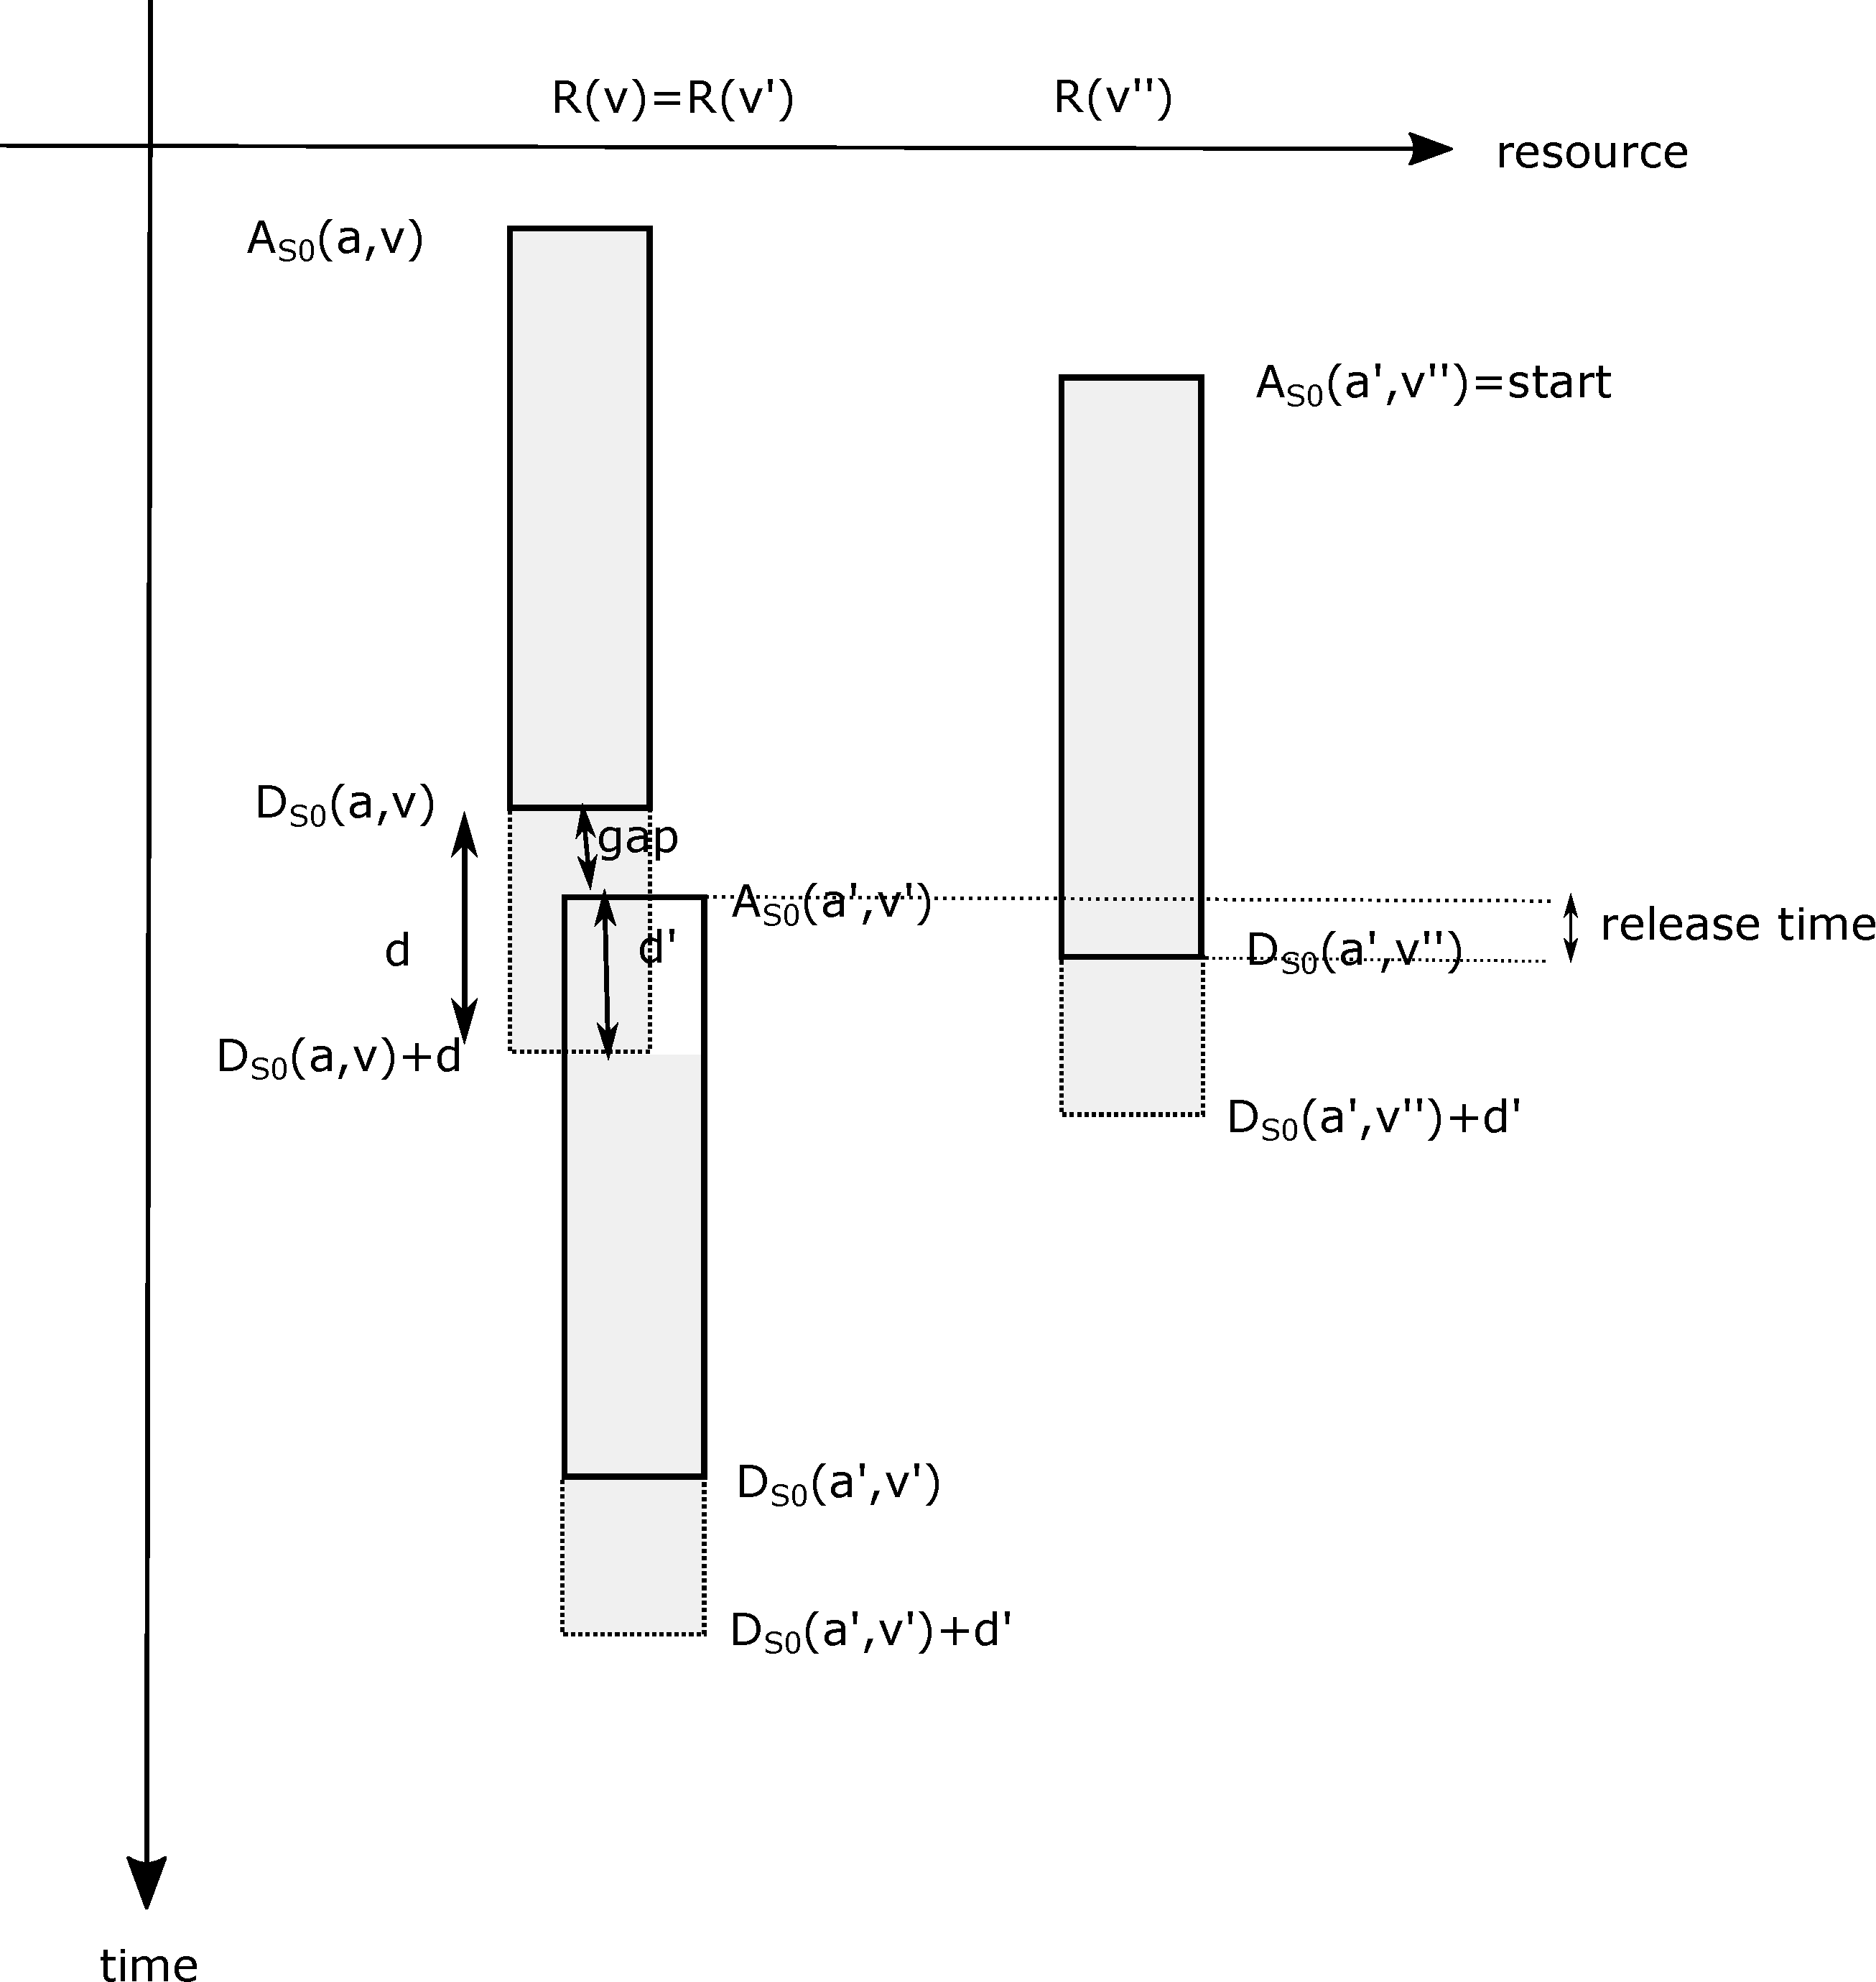
\includegraphics[width=\textwidth]{Figures/03_pipeline/transmission_chains.pdf}
	\caption{Illustration of transmission chains algorithms. The plain boxes represent the resource occupation of the schedule $S_0$, the dotted boxes represent the propagated delays, and the shaded areas represent the resource occupations with the propagated delay included. We assume that agents $a^\prime$ can stop immediately in the the cell $R(v^{\prime\prime}$ just before they are hit at $R(v)=R(v^\prime)$ enter through $v^\prime$ by the malfunction and that they do not decelerate earlier. Furthermore, we assume that agents $a^\prime$ on their course after $start$ can never compensate the propagated delay, i.e. that there are on time reserves that could decrease the propagated delay.}
	\label{fig:transmission_chains}
\end{figure}




Again, we conjecture\footnote{We do not prove it formally. The rationale is that every agent hit by the wave is opened up and this should allow for feasibility. The wave, can also move backwards in time in the range of the propagated delay reflecting a spill-back of congestion, see Figure~\ref{fig:transmission_chains}.} that this algorithms produces a feasible scope if $c >= malfunction duration$, in both cases with or without time flexibility.
%
We expect false negatives and false positives in our prediction: the delay may open up the opportunity for a second train to depart earlier (false positive), causing a third train to be only slightly delayed (false negative).


We call our delay propagation transmission chains because in the full implementation we not only store the delayed effect but the full chains. This makes debugging easier and allows to easily compute various statistics such as the level the source delay has first reached another agent.

Our approach is similar to delay propagation in \cite{handbookofoptimizationinrailwayindustry} where delay propagation is illustrated in the setting of event activity graphs with given decisions.

We could optimize the pseudo-code by ensuring that only the largest delay of an agent at a resource is in the queue; we have refrained from this to keep the exposition simple.

%%%%%%%%%%%%%%%%%%%%%%%%%%%%%%%%%%%%%%%%%%%%%%%%%%%%%%%%%%%%%%%%%%%%%%%%%%
\subsubsection{Random Online Re-scheduling (online\_random)}
\label{subsubsec:scope_online_random}
%%%%%%%%%%%%%%%%%%%%%%%%%%%%%%%%%%%%%%%%%%%%%%%%%%%%%%%%%%%%%%%%%%%%%%%%%%

As a sanity check, to show that our scoping is not trivial, we use Algorithm~\ref{algo:scoper_changed} with random prediction of Algorithm~\ref{algo:scoper_random}: we determine the fraction of changed agents among those running at or after the malfunction (lines 1--2) and choose randomly with the same fraction among those running after the malfunction, ensuring that the malfunction agent is contained (lines 3--7).


\begin{algorithm}
	\caption{$scoper\_offline\_random$} \label{algo:scoper_random}
	\begin{algorithmic}[1]
		\Require $\mathcal{A}$, $(P_{S_0},A_{S_0})$,$M=(m_{time\_step},m_{duration},m_{agent})$,$v$,$U$,$U$,$c$, $(P_S,A_S)$
	    \Ensure $\mathcal{A}$
	    \State $\mathcal{A}_{running}=\Set{a \in \mathcal{A}: \max_{v \in P_{S_0}} A_{S_0}(a,v) \geq m_{time\_step}}$
	    \State $n_{changed} = \left| \Set{a\in \mathcal{A}_{running}:  P_{S_0} \not=P_{S} \textrm { or } A_{S_0}(a,\cdot) \not= A_{S}(a,\cdot)} \right|$
	    \State $\mathcal{A}^* \leftarrow$ choose $n_{changed}$ from $\mathcal{A}_{running}$
	    \State $\mathcal{A}^* \leftarrow scoper\_changed(\mathcal{A},(P_{S_0},A_{S_0}),\mathcal{A}^*,time\_flexibility=\top,v,U,c)$
	\end{algorithmic}
\end{algorithm}
The output of this prediction can then be passed to Algorithm~\ref{algo:scoper_changed} with time flexibility to determine the re-scheduling problem.
Again, we conjecture that this algorithms produces a feasible scope if $c >= m_{duration}$ (without time flexibility, there is clearly no guarantee of feasibility).


%%%%%%%%%%%%%%%%%%%%%%%%%%%%%%%%%%%%%%%%%%%%%%%%%%%%%%%%%%%%%%%%%%%%%%%%%%
%%%%%%%%%%%%%%%%%%%%%%%%%%%%%%%%%%%%%%%%%%%%%%%%%%%%%%%%%%%%%%%%%%%%%%%%%%
\section{Computational Results}\label{sec:Results}
%%%%%%%%%%%%%%%%%%%%%%%%%%%%%%%%%%%%%%%%%%%%%%%%%%%%%%%%%%%%%%%%%%%%%%%%%%
%%%%%%%%%%%%%%%%%%%%%%%%%%%%%%%%%%%%%%%%%%%%%%%%%%%%%%%%%%%%%%%%%%%%%%%%%%




%%%%%%%%%%%%%%%%%%%%%%%%%%%%%%%%%%%%%%%%%%%%%%%%%%%%%%%%%%%%%%%%%%%%%%%%%%
\subsection{Experiment Design}
%%%%%%%%%%%%%%%%%%%%%%%%%%%%%%%%%%%%%%%%%%%%%%%%%%%%%%%%%%%%%%%%%%%%%%%%%%

In light of the findings of the previous paragraphs, we design our experiments in a hierarchical fashion on multiple levels
\begin{enumerate}
    \item infrastructure
    \item schedule
    \item malfunction
    \item solver runs
\end{enumerate}
where at each level we generate multiple instances for a fixed instance of the previous levels (i.e. we generate multiple infrastructures for the same parameters, we generate multiple schedules for the same infrastructure etc.). The lowest level is a sanity level to investigate the variance of the solver for the same problem.

In order to show the speed-up, we want our problems to cover a good range of problems.
These considerations lead us  to the following agenda for this section, as shown in Figure~\ref{fig:agenda}. The full parameter ranges are shown in Appendix~\ref{subsec:experiment_parameters}.
%

We take our  baseline (online unrestricted) as  measure of the hardness of our problems; in Figure~\ref{fig:agenda_histogram}, we see that our experiments are biased to the left, i.e. it is hard to choose parameters such the problems get harder -- we see no correlation between the experiment id (which reflects the infrastructure size) and online unrestricted.

\begin{figure}[hbtp]
    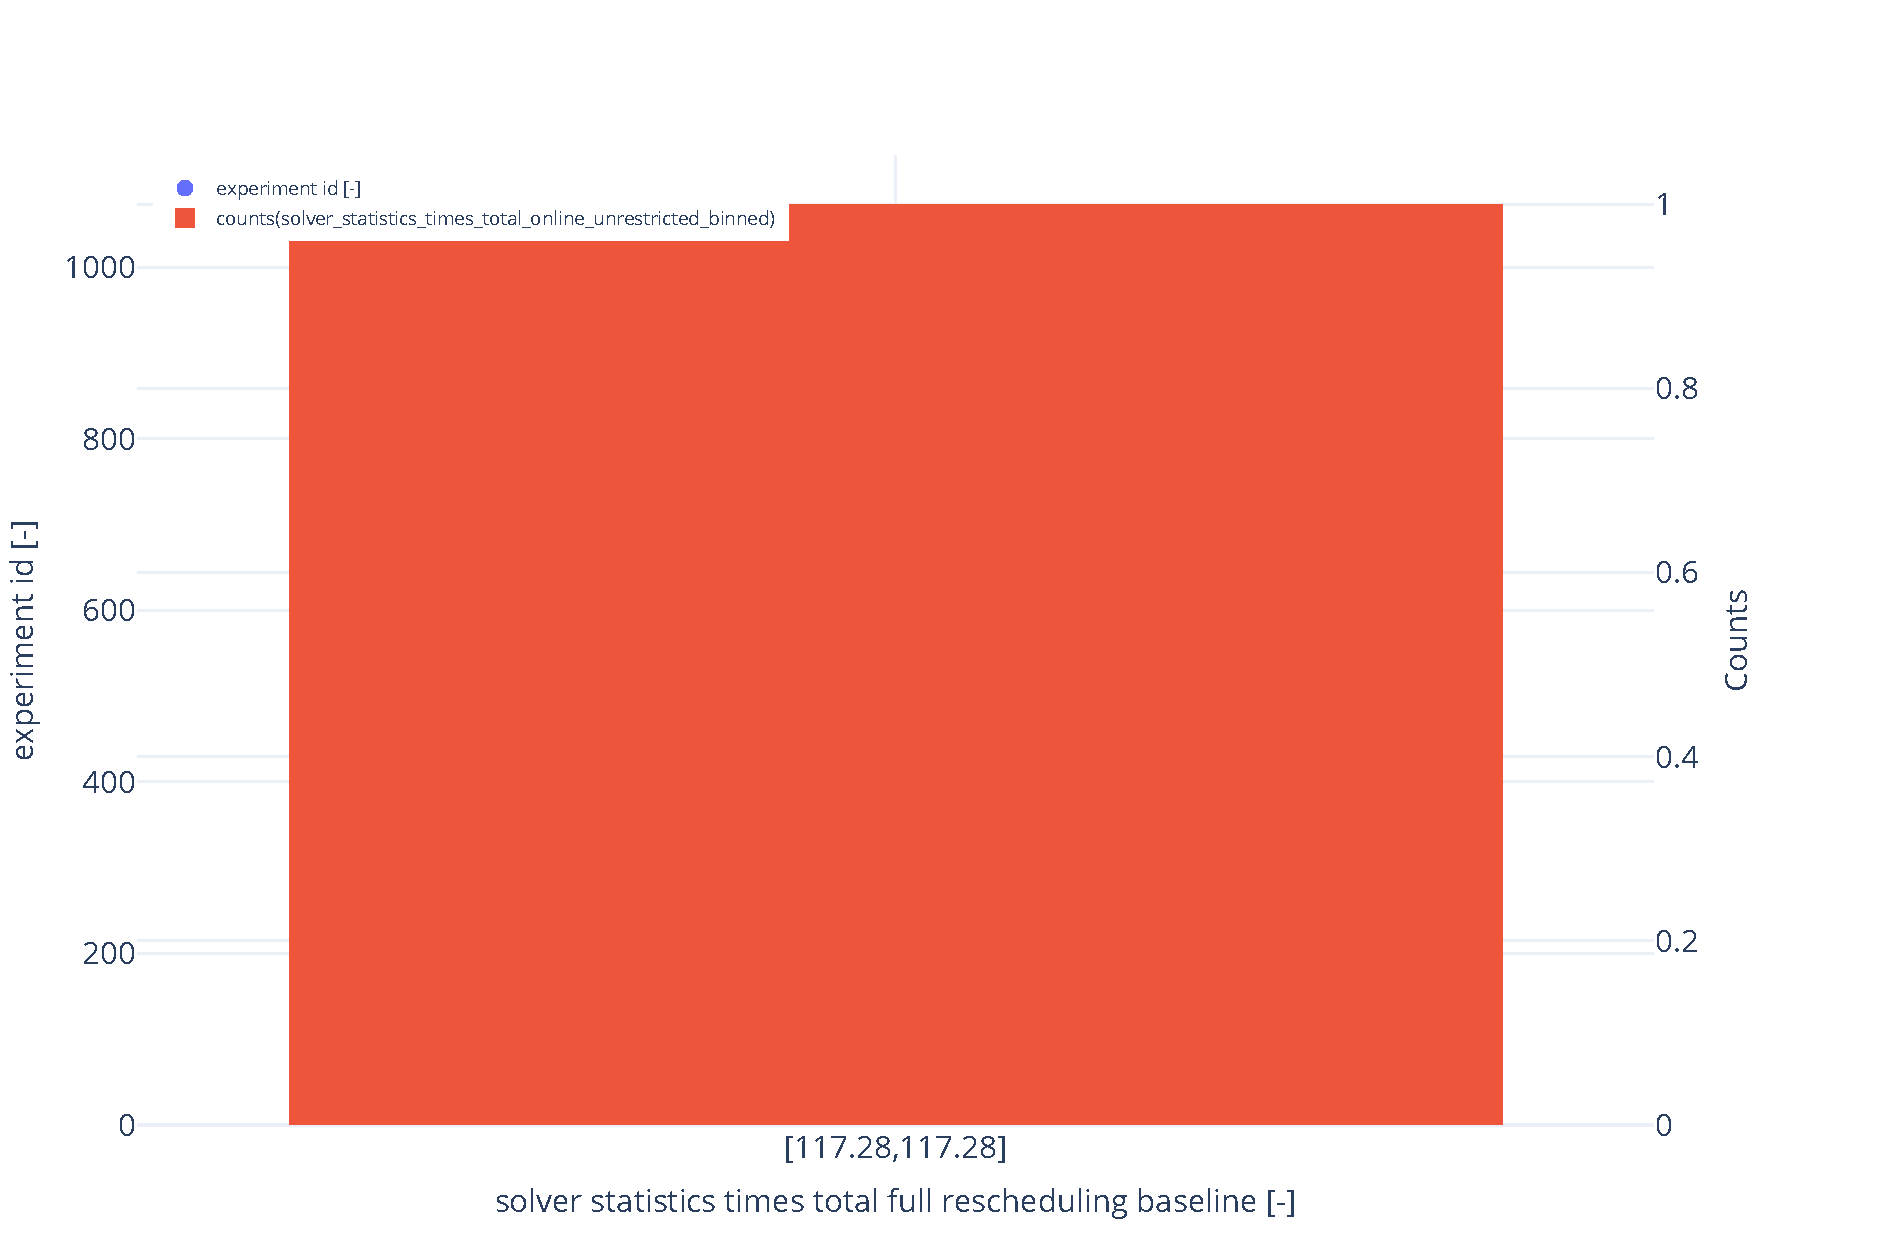
\includegraphics[width=\textwidth]{Figures/04_computational_results/times_total_histogram.pdf}
	\caption{Histogram of experiments in 10 equi-distant bins, filtered on data with \texttt{solver\_statistics\_times\_total\_online\_unrestricted} between $20s$ and $200s$.}
	\label{fig:agenda_histogram}
\end{figure}




%We filter out  experiments with small absolute and large relative run times:
%\begin{itemize}
%    \item time full after malfunction $< 10$s
%    \item time full after malfunction $> 97\%$-percentile of time full after malfunction
%\end{itemize}
%This filters out 68 experiments and leaves us with data from 312 experiments.
We filter out experiments with small and large run times (if the solver took less than $20s$ or more than $200s$ for the online unrestricted scope; this leaves us with 125 data points.

\begin{figure}[hbtp]
    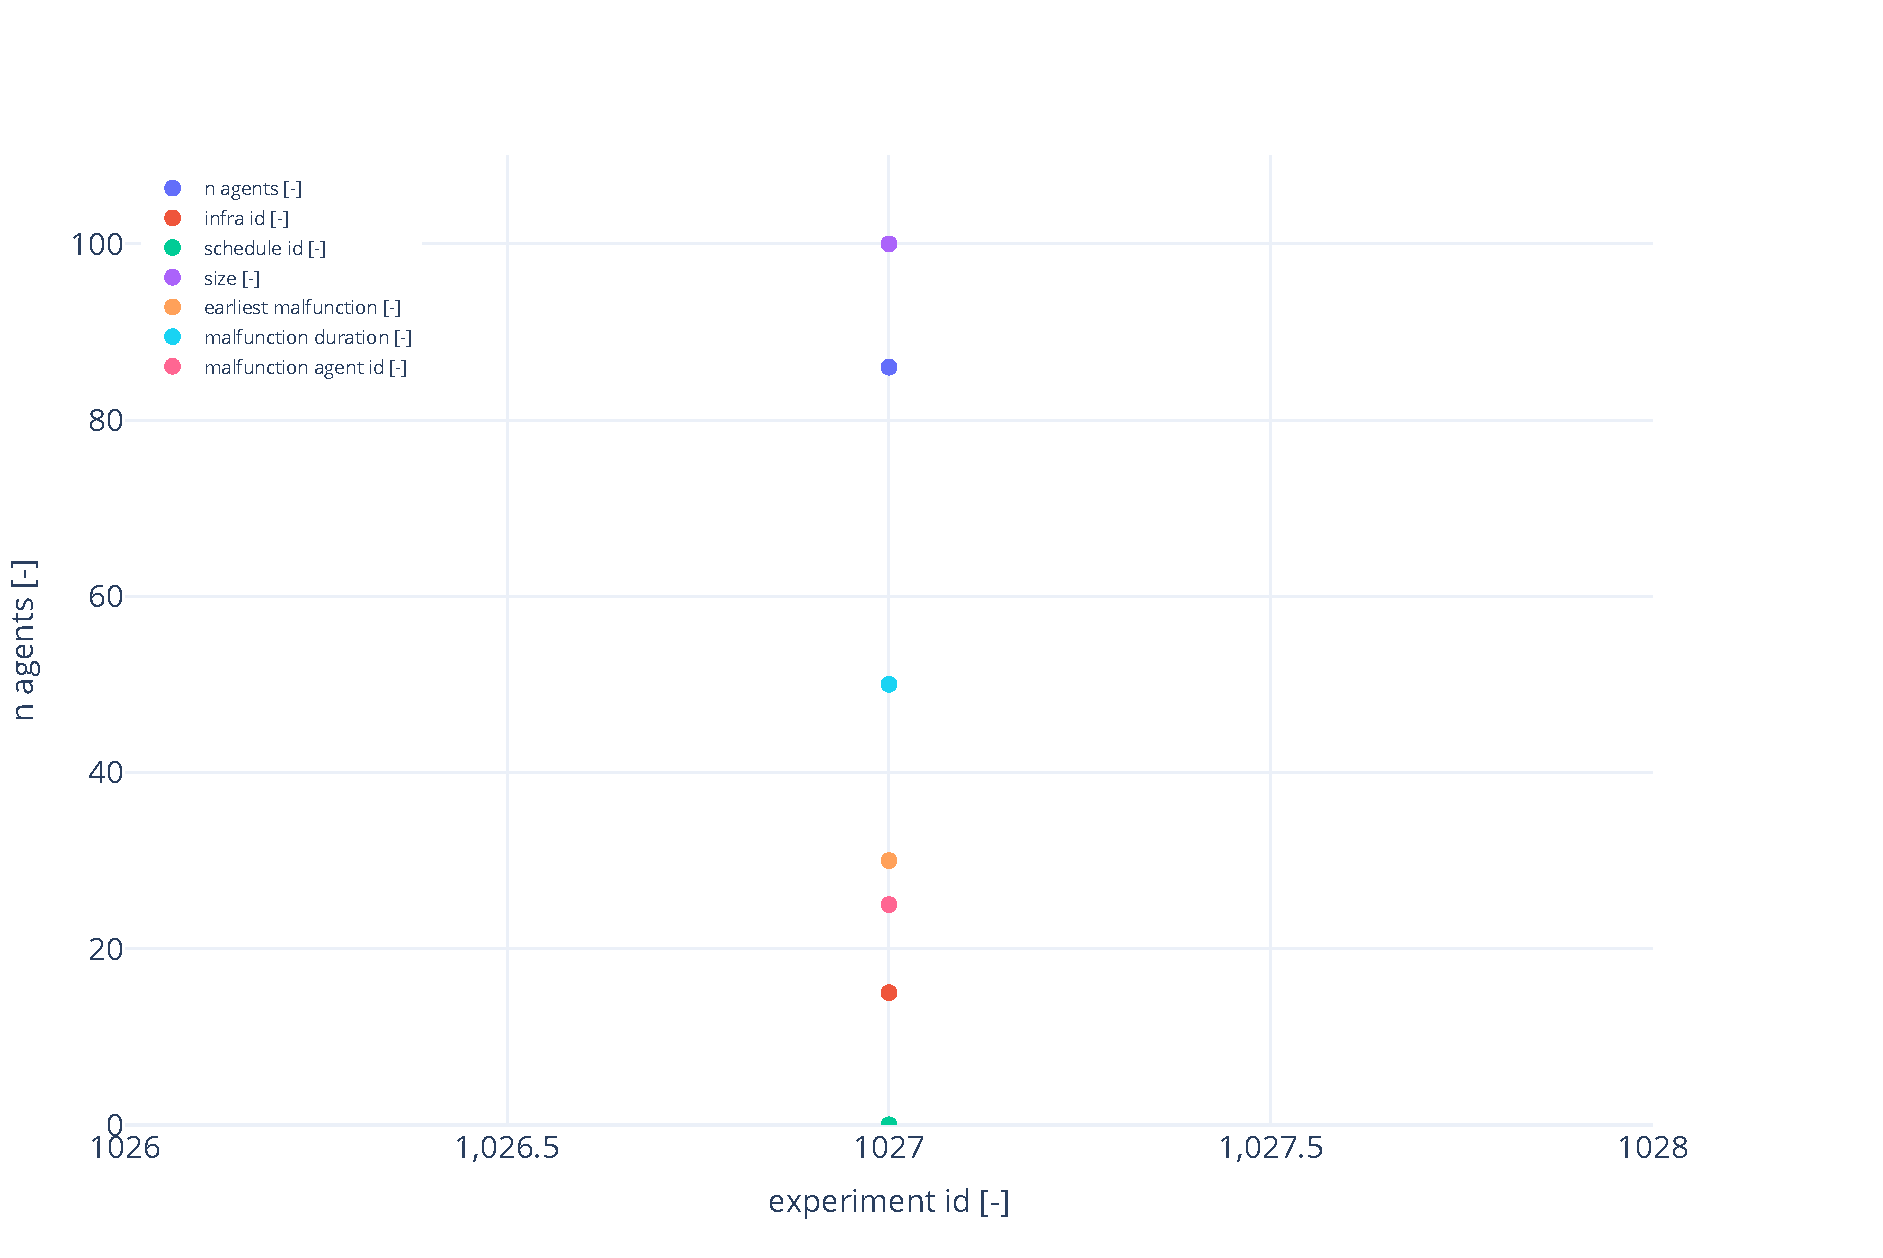
\includegraphics[width=\textwidth]{Figures/04_computational_results/agenda.pdf}
	\caption{Hierarchical Agenda Structure.}
	\label{fig:agenda}
\end{figure}




%%%%%%%%%%%%%%%%%%%%%%%%%%%%%%%%%%%%%%%%%%%%%%%%%%%%%%%%%%%%%%%%%%%%%%%%%%
\subsection{Speed-Up and Solution Quality}
%%%%%%%%%%%%%%%%%%%%%%%%%%%%%%%%%%%%%%%%%%%%%%%%%%%%%%%%%%%%%%%%%%%%%%%%%%

\begin{figure}[hbtp]
    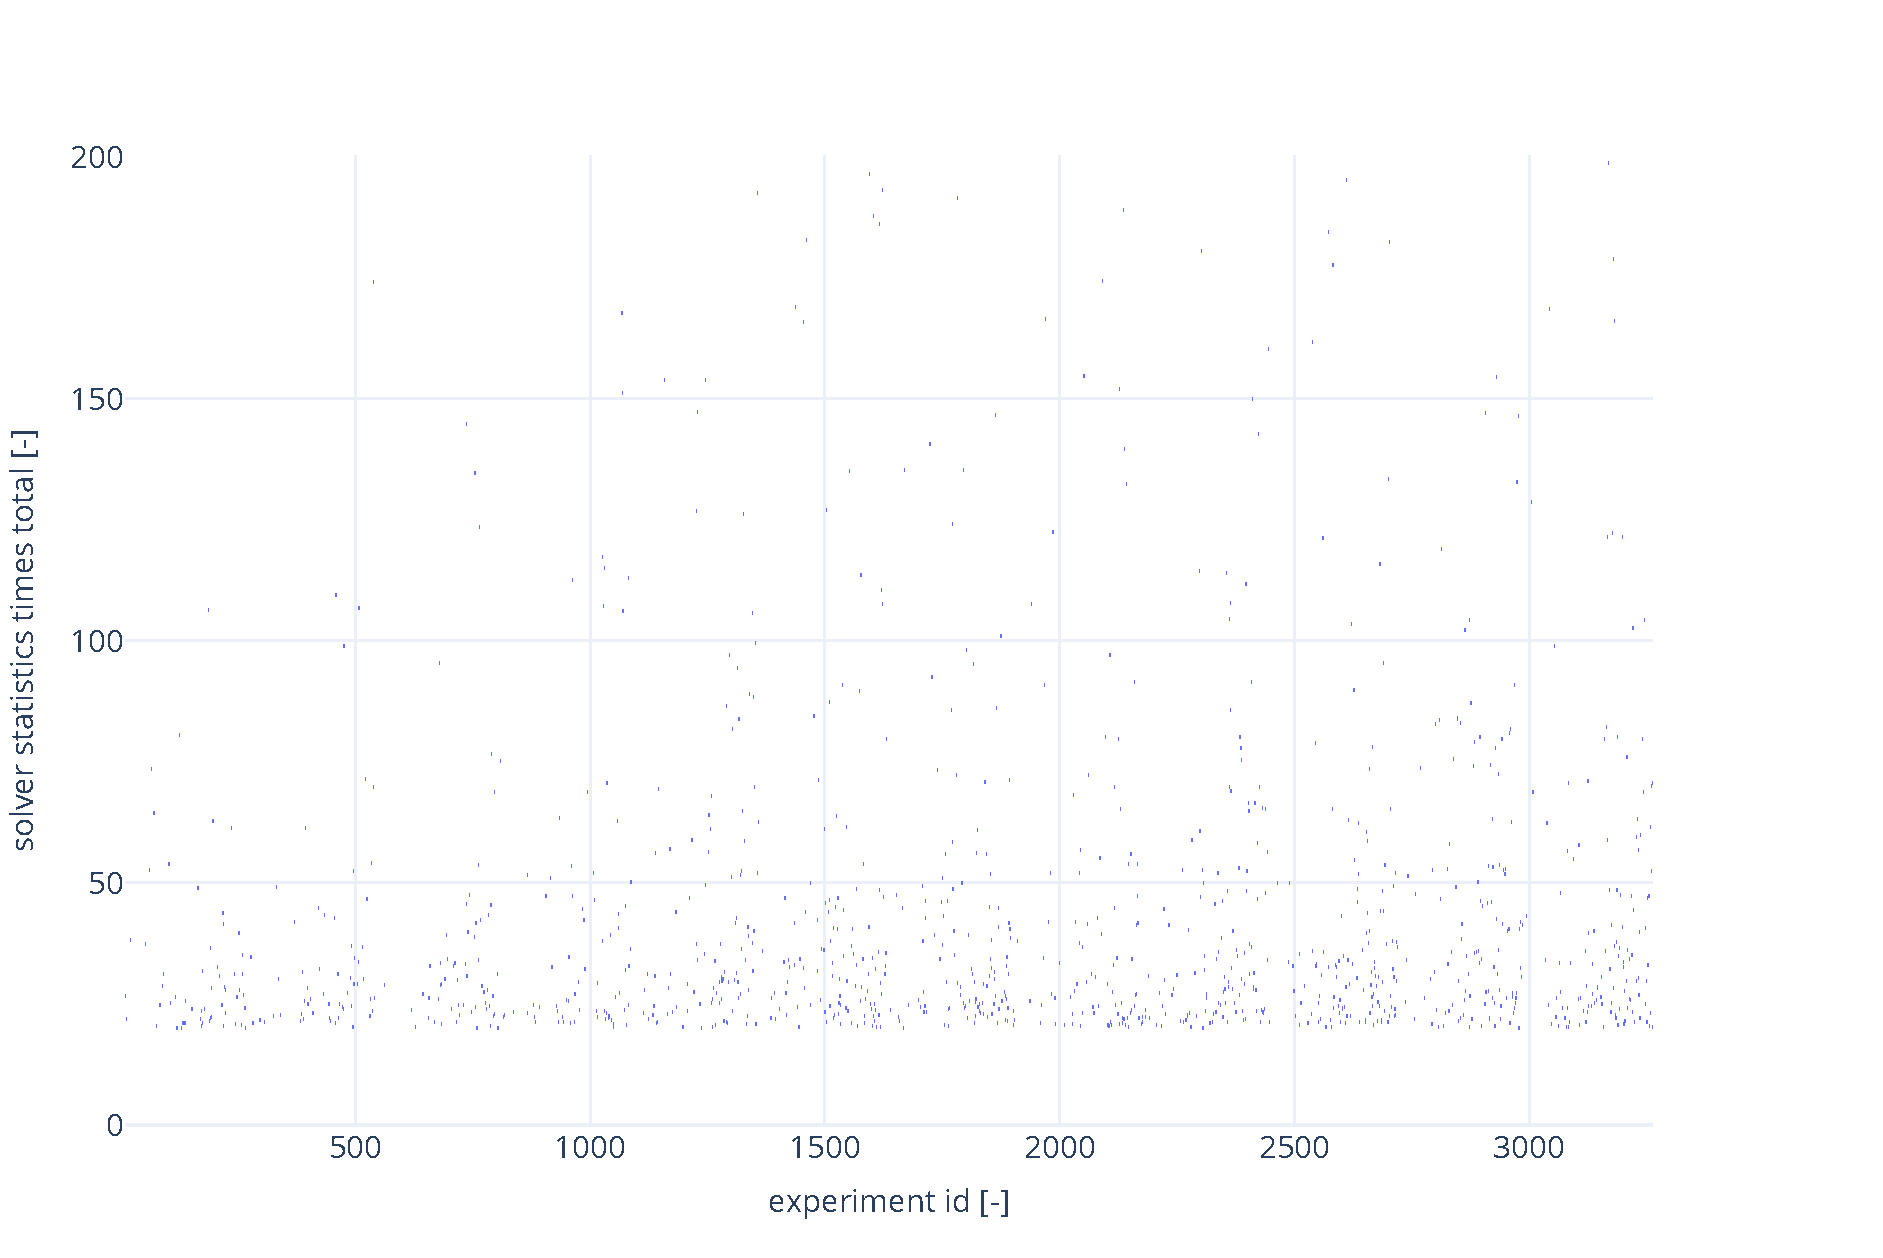
\includegraphics[width=\textwidth]{Figures/04_computational_results/times_total_per_experiment_id.pdf}
	\caption{Computation times per experiment.}
	\label{fig:computationtimesexperimentid}
\end{figure}
In Figure~\ref{fig:computationtimesexperimentid}, we do not recognize any block structure of running times as we could expect from Figure~\ref{fig:agenda}. In other words, grid size and number of agents are not a good measure of the difficulty of the re-scheduling problem (we conjecture that it may be even hard to determine beforehand whether a problem is hard); furthermore, the difficulty varies greatly for the same schedule when taking different agents (notice that this implies different time steps as well since the malfunction is performed 30 time steps after the malfunction agent's departure); also other indicators as the number of agents running after the malfunction or the time horizon remaining after the malfunction did not give any hint on re-scheduling time (online unrestricted). We will come back to this in Section~\ref{sec:CaseStudies}, where we give some illustrations.

Therefore, we for lack of a better take the full re-scheduling time (online unrestricted) as measure of problem complexity and plot the rescheduling times and speed-up for the different scopes against the full re-scheduling time in Figures~\ref{fig:computationtimes}, \ref{fig:speed_up} and \ref{fig:solve_non_solve}.
We see a clear separation and increase of speed-up for larger online unrestricted in the following order:
\begin{enumerate}
    \item online fully restricted
    \item offline delta
    \item online route restricted
\end{enumerate}
We see a small speed-up for random and none for our transmission chains approach. We believe the small speed-up for random comes from randomly choosing agents whose paths are restricted.





\begin{figure}[hbtp]
	\begin{subfigure}{\textwidth}
        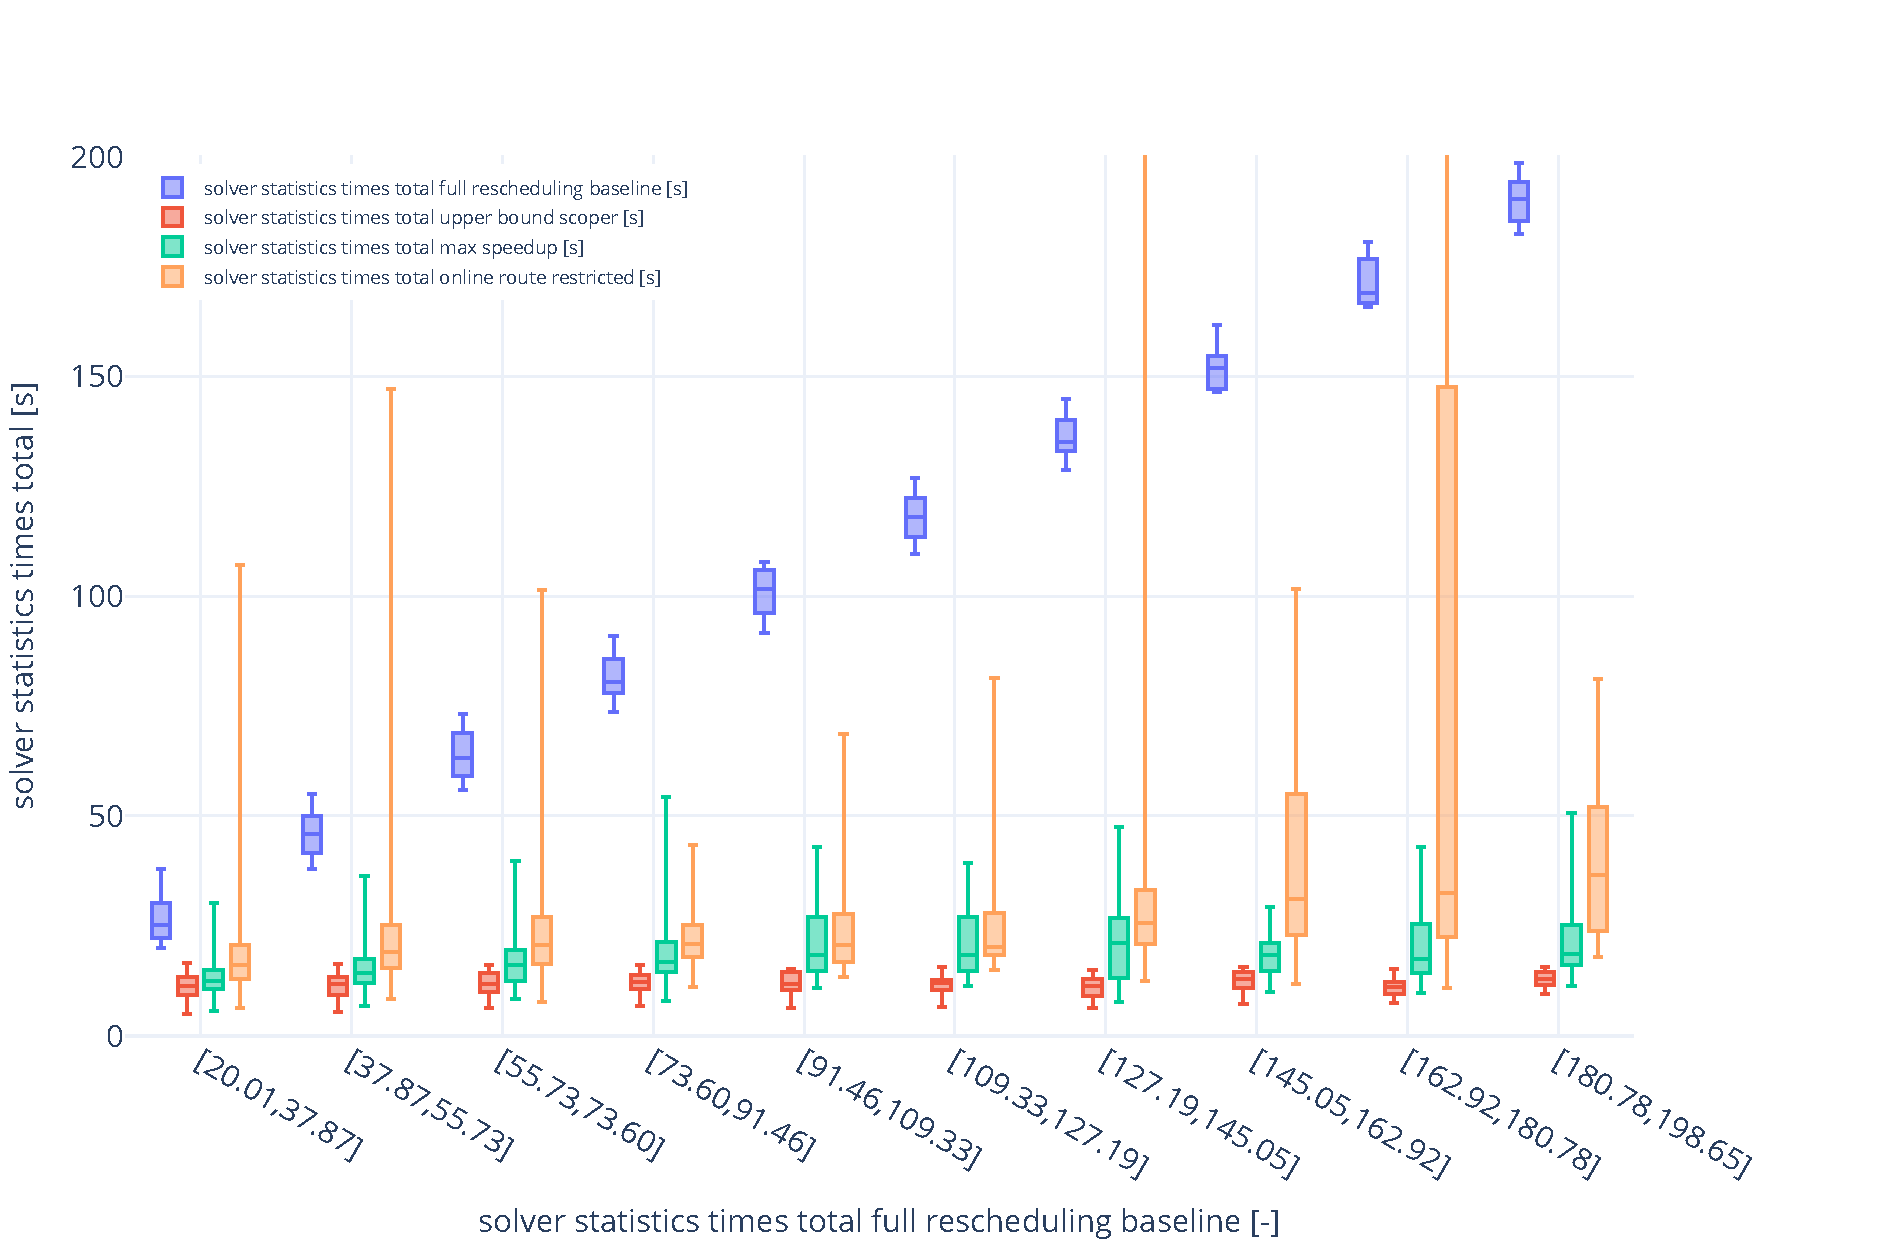
\includegraphics[width=\textwidth]{Figures/04_computational_results/times_total_per_times_total_online_unrestricted_1.pdf}
        \caption{Total solver runtimes for online unrestricted, online full restricted, offline delta and online route restricted}
        \label{fig:computationtimes_absolute_1}
    \end{subfigure}

    \begin{subfigure}{\textwidth}
          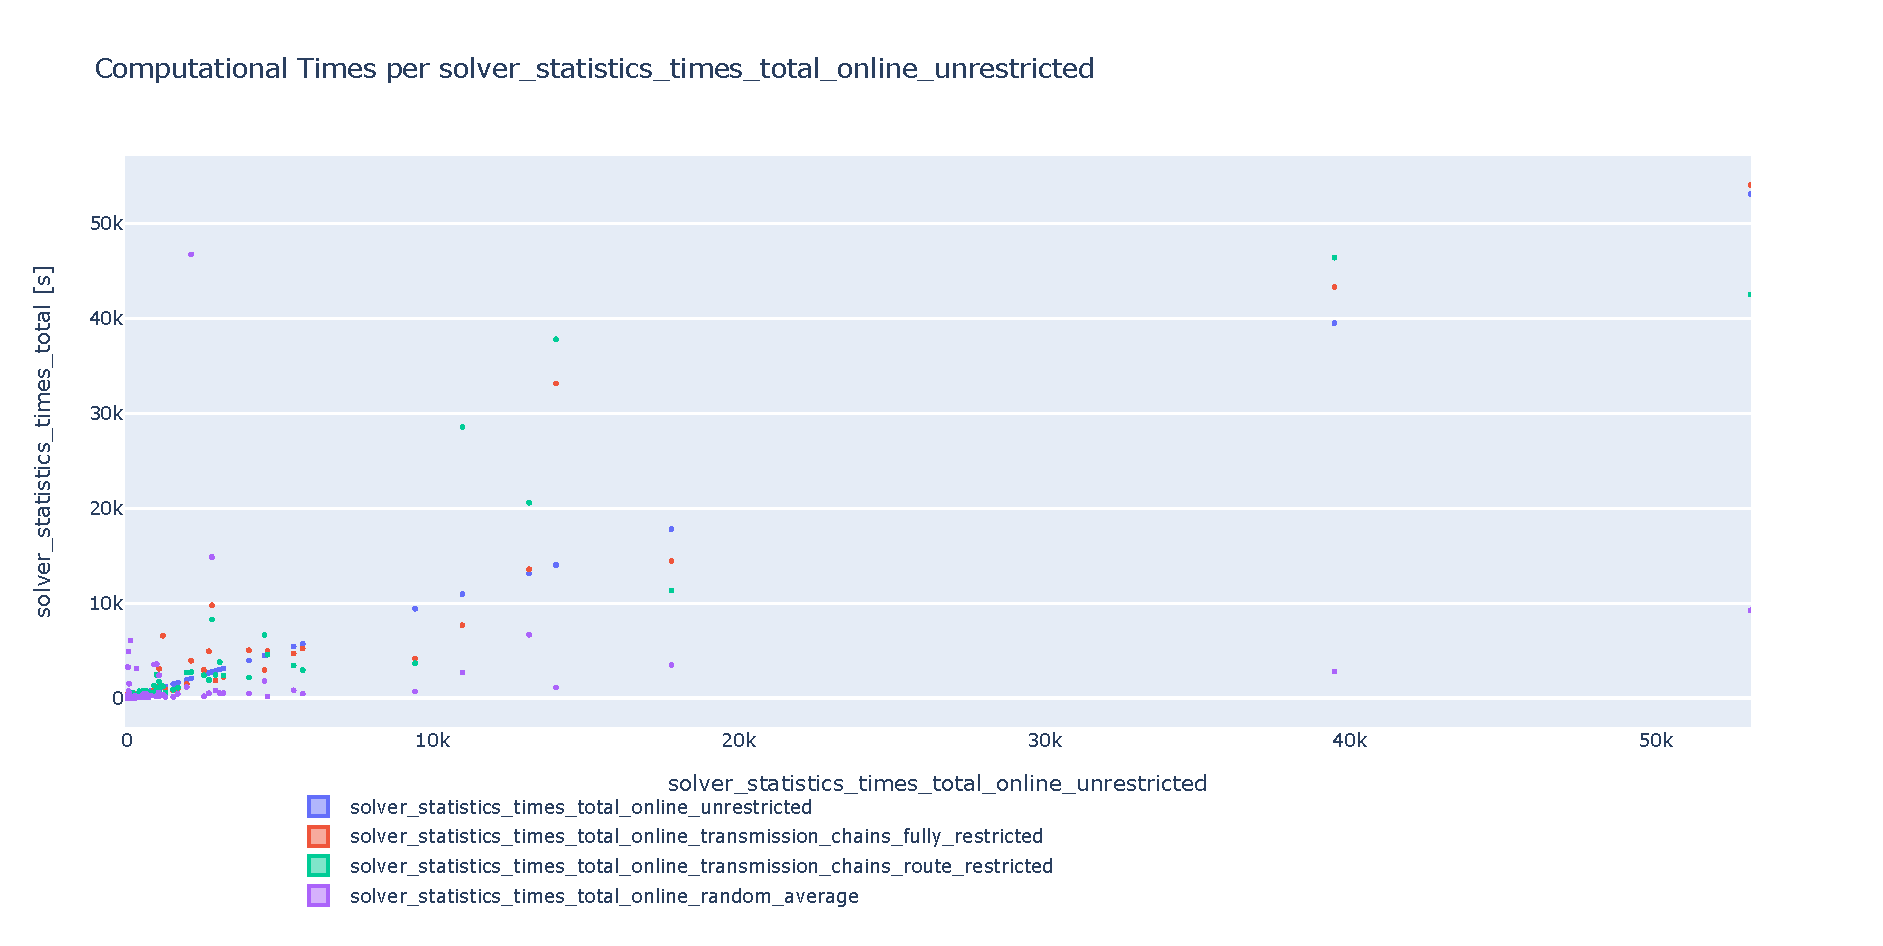
\includegraphics[width=\textwidth]{Figures/04_computational_results/times_total_per_times_total_online_unrestricted_2.pdf}
          \label{fig:computationtimes_absolute_2}
          \caption{Total solver runtimes for online transmissions chains and online random against online unrestricted.}
     \end{subfigure}
	\caption{Re-scheduling times against full re-scheduling time.}
	\label{fig:computationtimes}
\end{figure}

\begin{figure}[hbtp]

     \begin{subfigure}{\textwidth}
        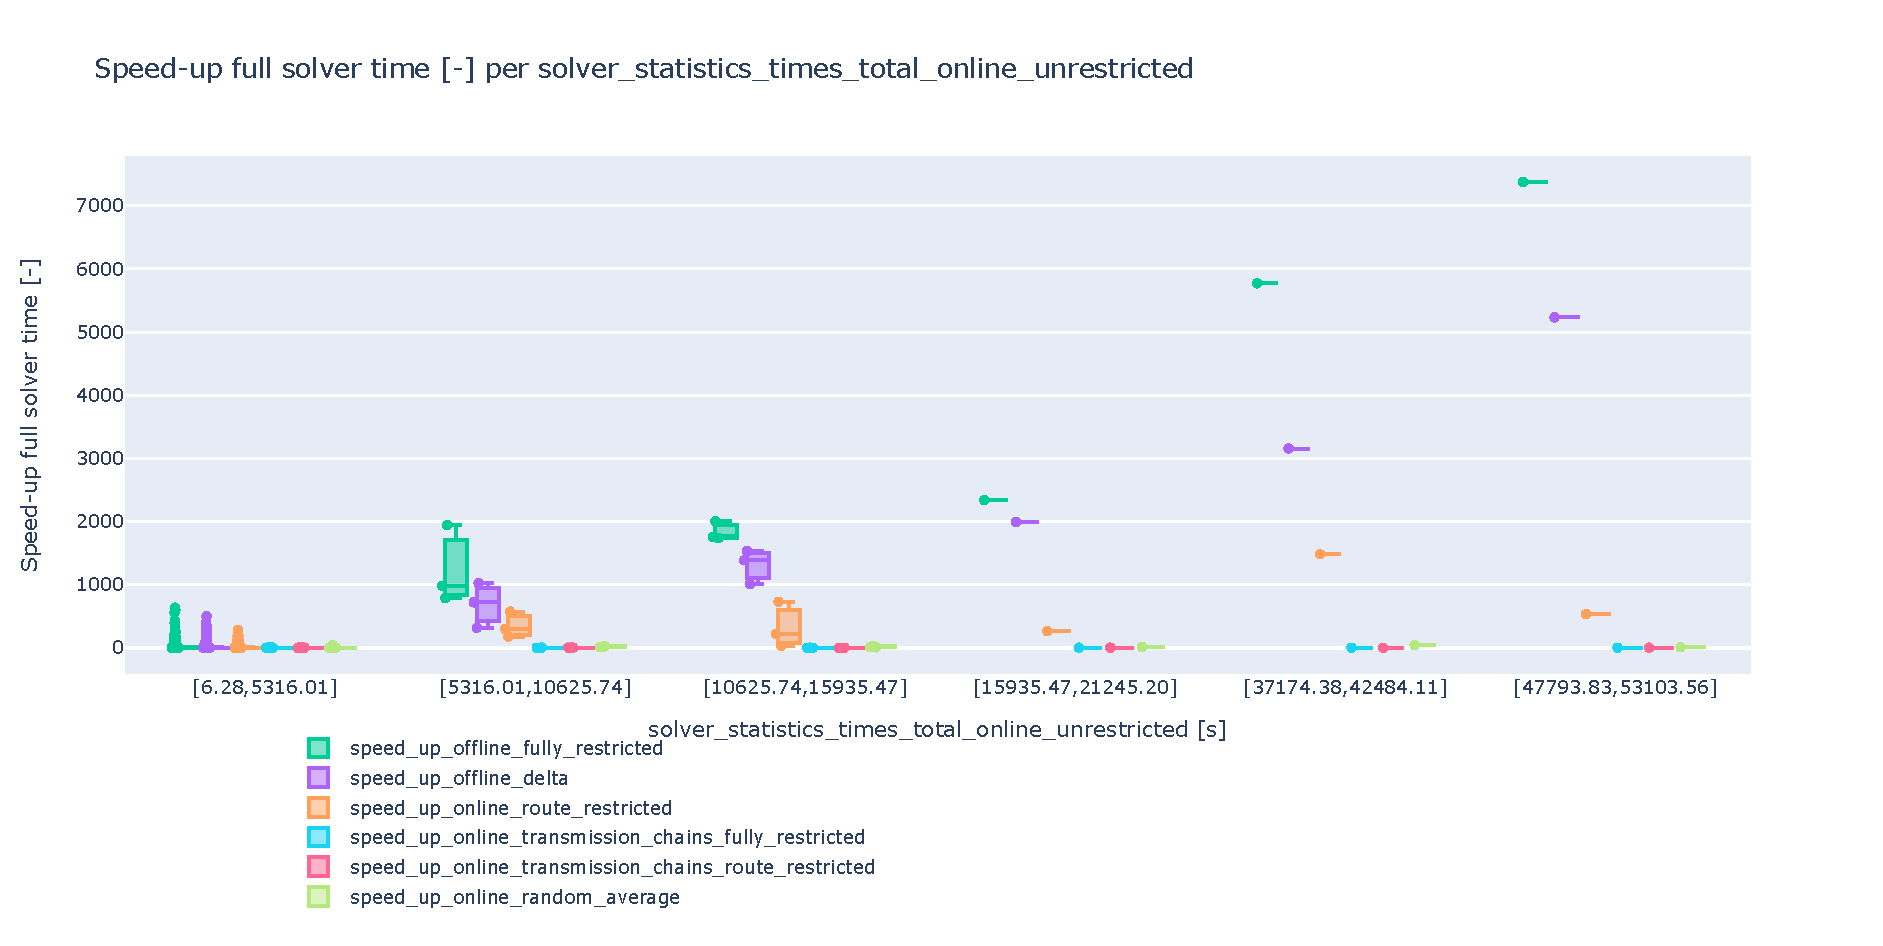
\includegraphics[width=\textwidth]{Figures/04_computational_results/speed_up_per_times_total_online_unrestricted.pdf}
        \caption{Speed-up for total solver time}
         \label{fig:computationtimes_speed_up_total}
    \end{subfigure}
     \begin{subfigure}{\textwidth}
        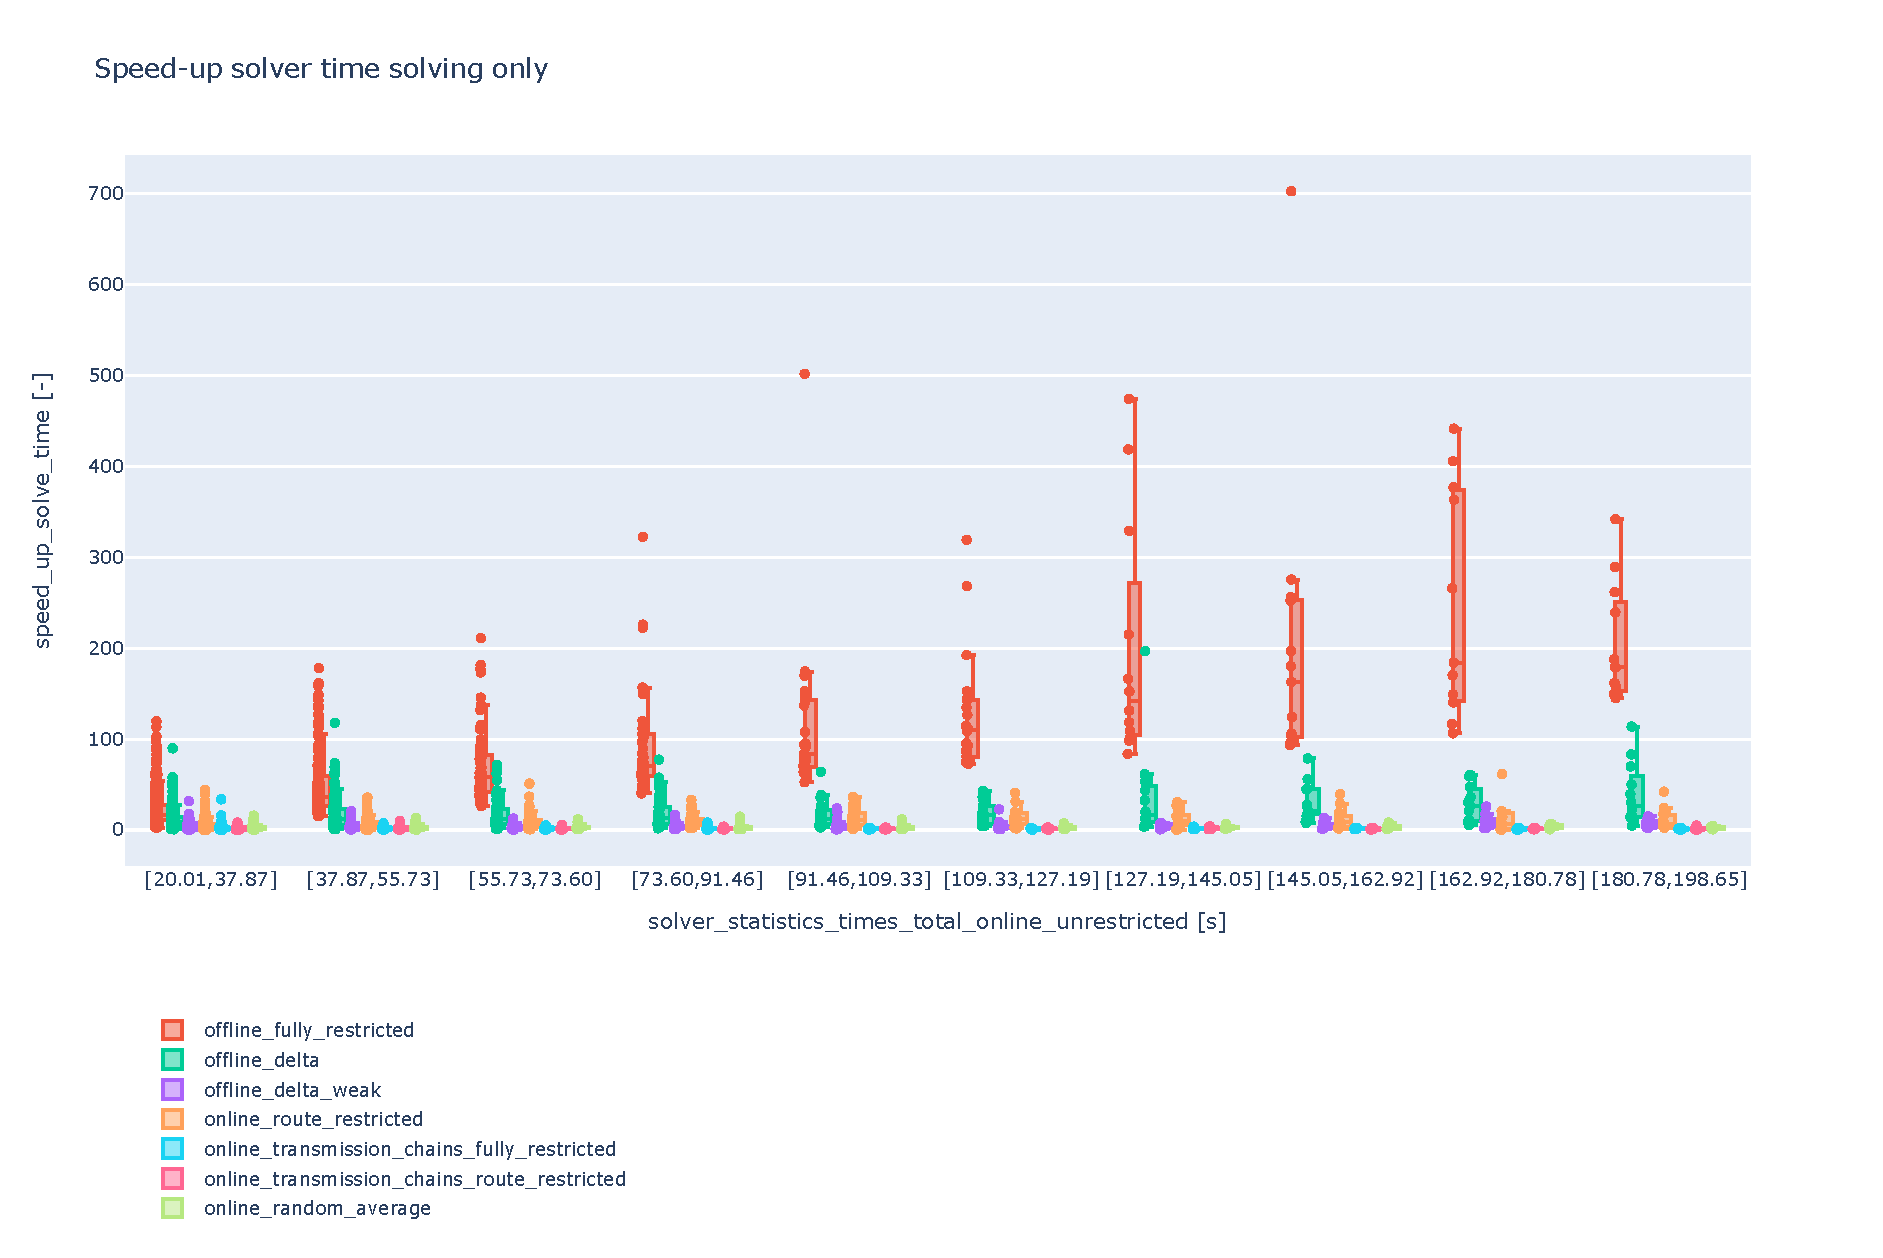
\includegraphics[width=\textwidth]{Figures/04_computational_results/speed_up_solve_time_per_times_total_online_unrestricted.pdf}
        \caption{Speed-up for solver time spent solving}
         \label{fig:computationtimes_speed_up_solve_time}
    \end{subfigure}
    \begin{subfigure}{\textwidth}
        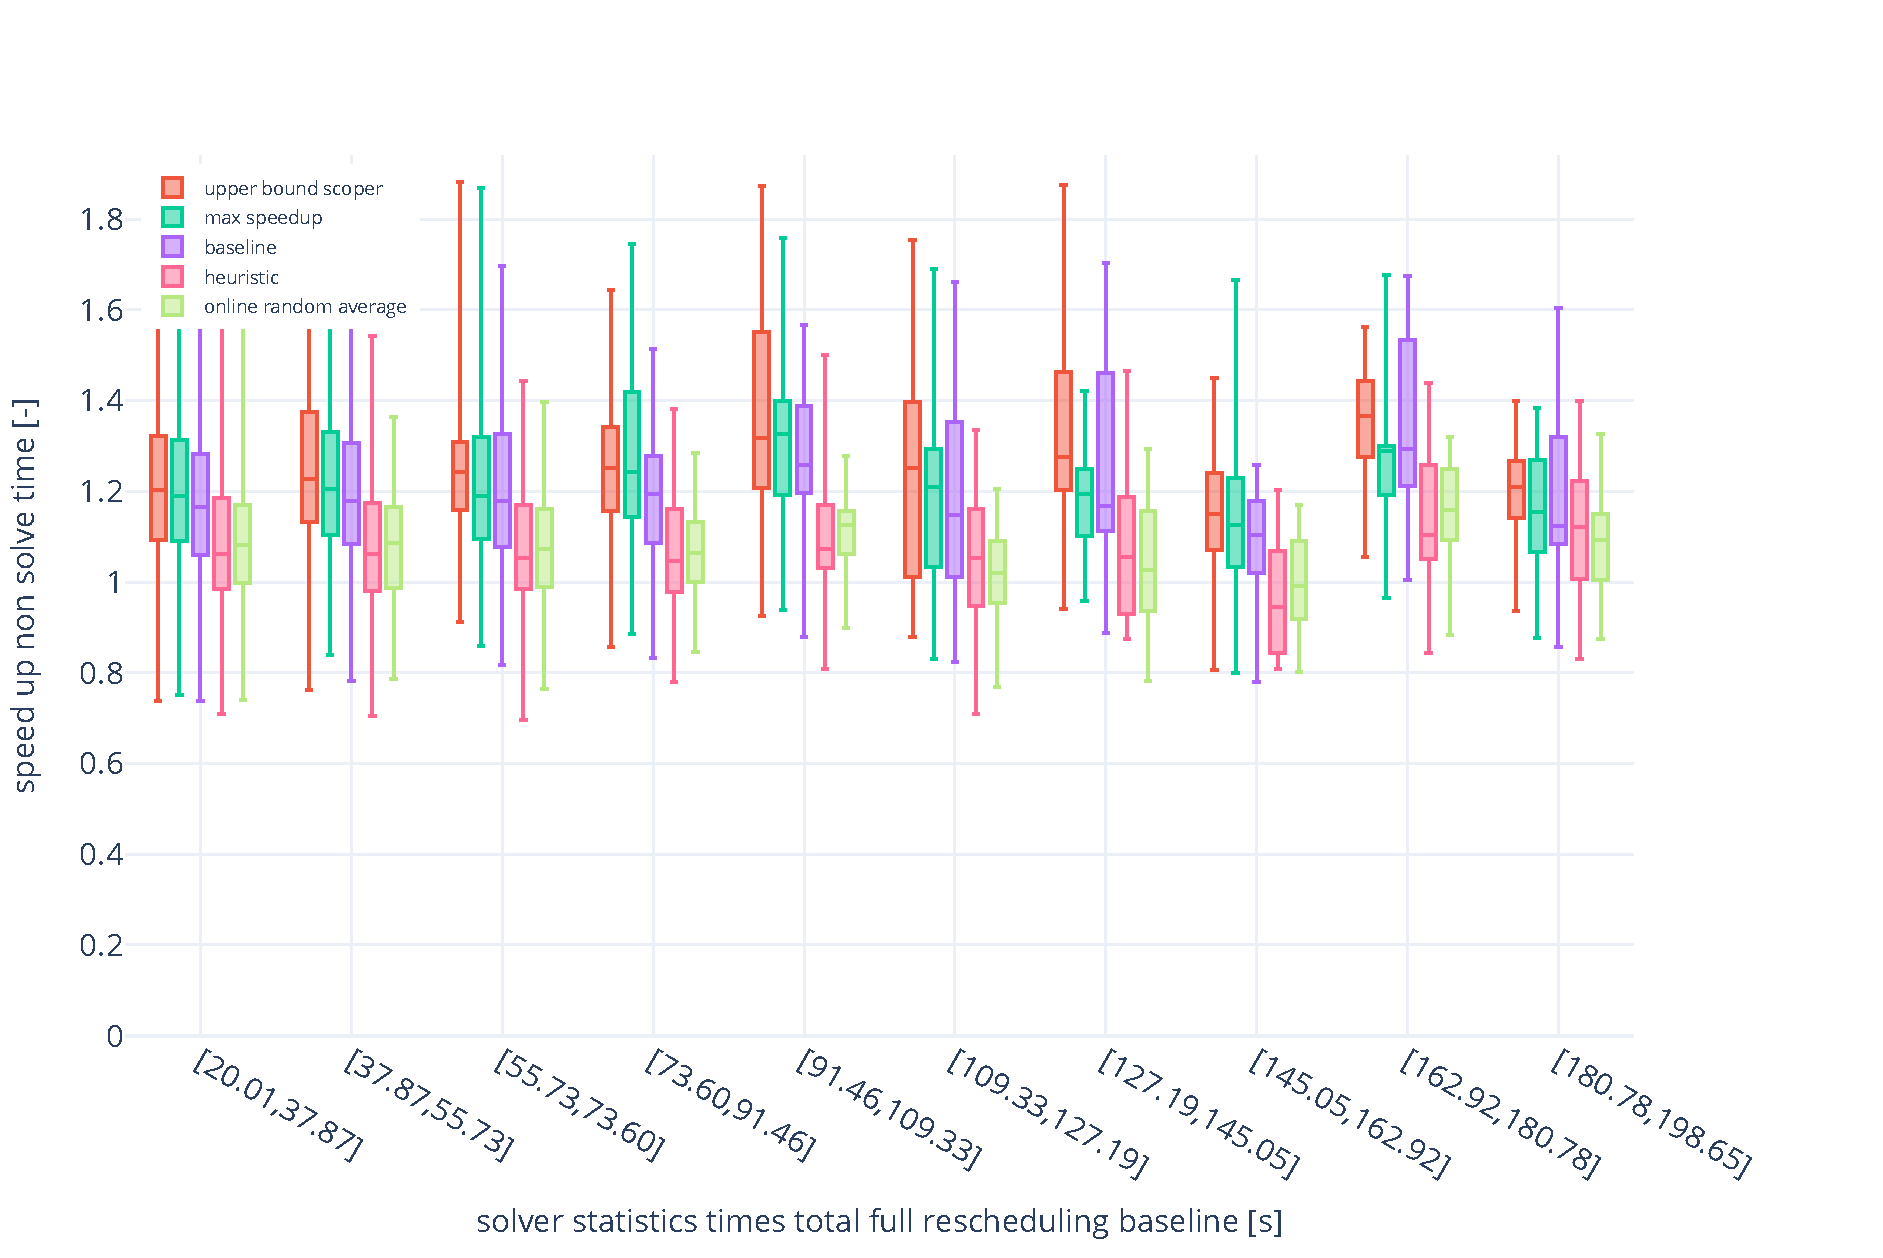
\includegraphics[width=\textwidth]{Figures/04_computational_results/speed_up_non_solve_time_per_times_total_online_unrestricted.pdf}
        \caption{Speed-up for total solver time spent non-solving}
         \label{fig:computationtimes_speed_up_non_solve_time}
    \end{subfigure}
	\caption{Speed-up of total solver time, solve time and non-solve time of the ASP solver. The speed-ups are grouped in 10 bins of equal size on the horizontal axis between min and max value.}
	\label{fig:speed_up}
\end{figure}


\begin{figure}[hbtp]
    \begin{subfigure}{\textwidth}
        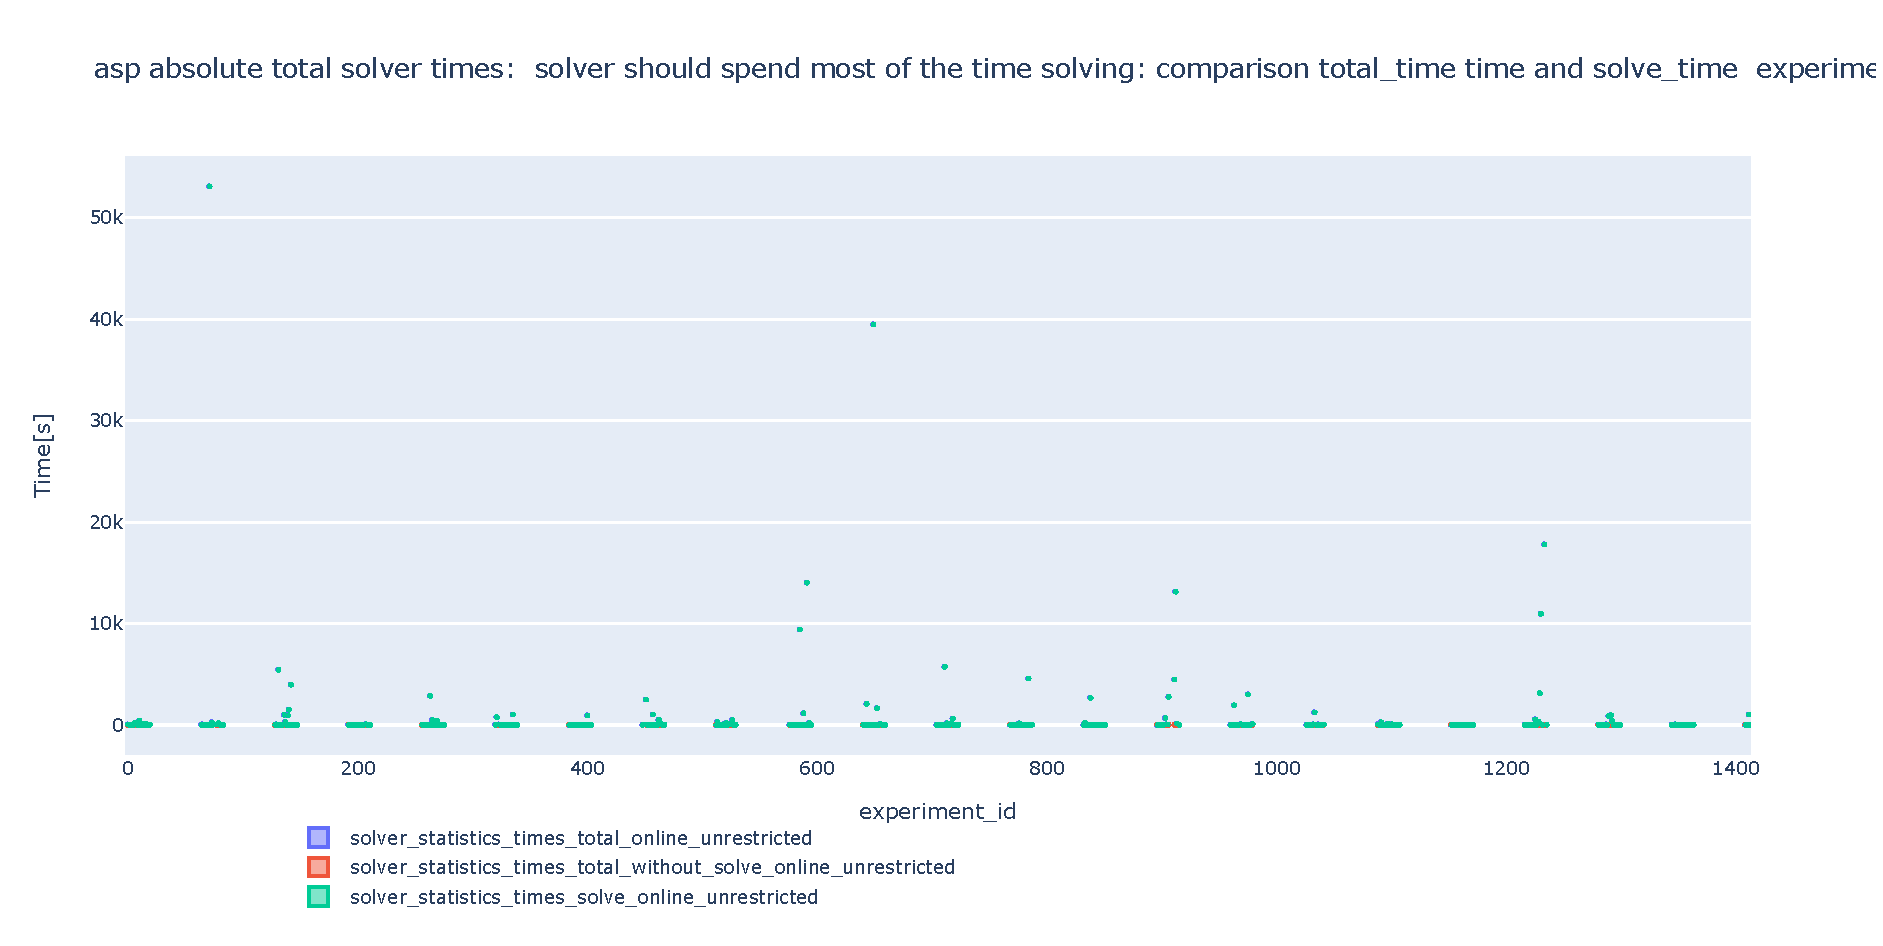
\includegraphics[width=\textwidth]{Figures/04_computational_results/solve_non_solve_online_unrestricted.pdf}
        \caption{Total solver time, solve time and non-solve time for online unrestricted}
         \label{fig:computationtimes_solve_non_solve_time_online_unrestricted}
    \end{subfigure}
    \begin{subfigure}{\textwidth}
        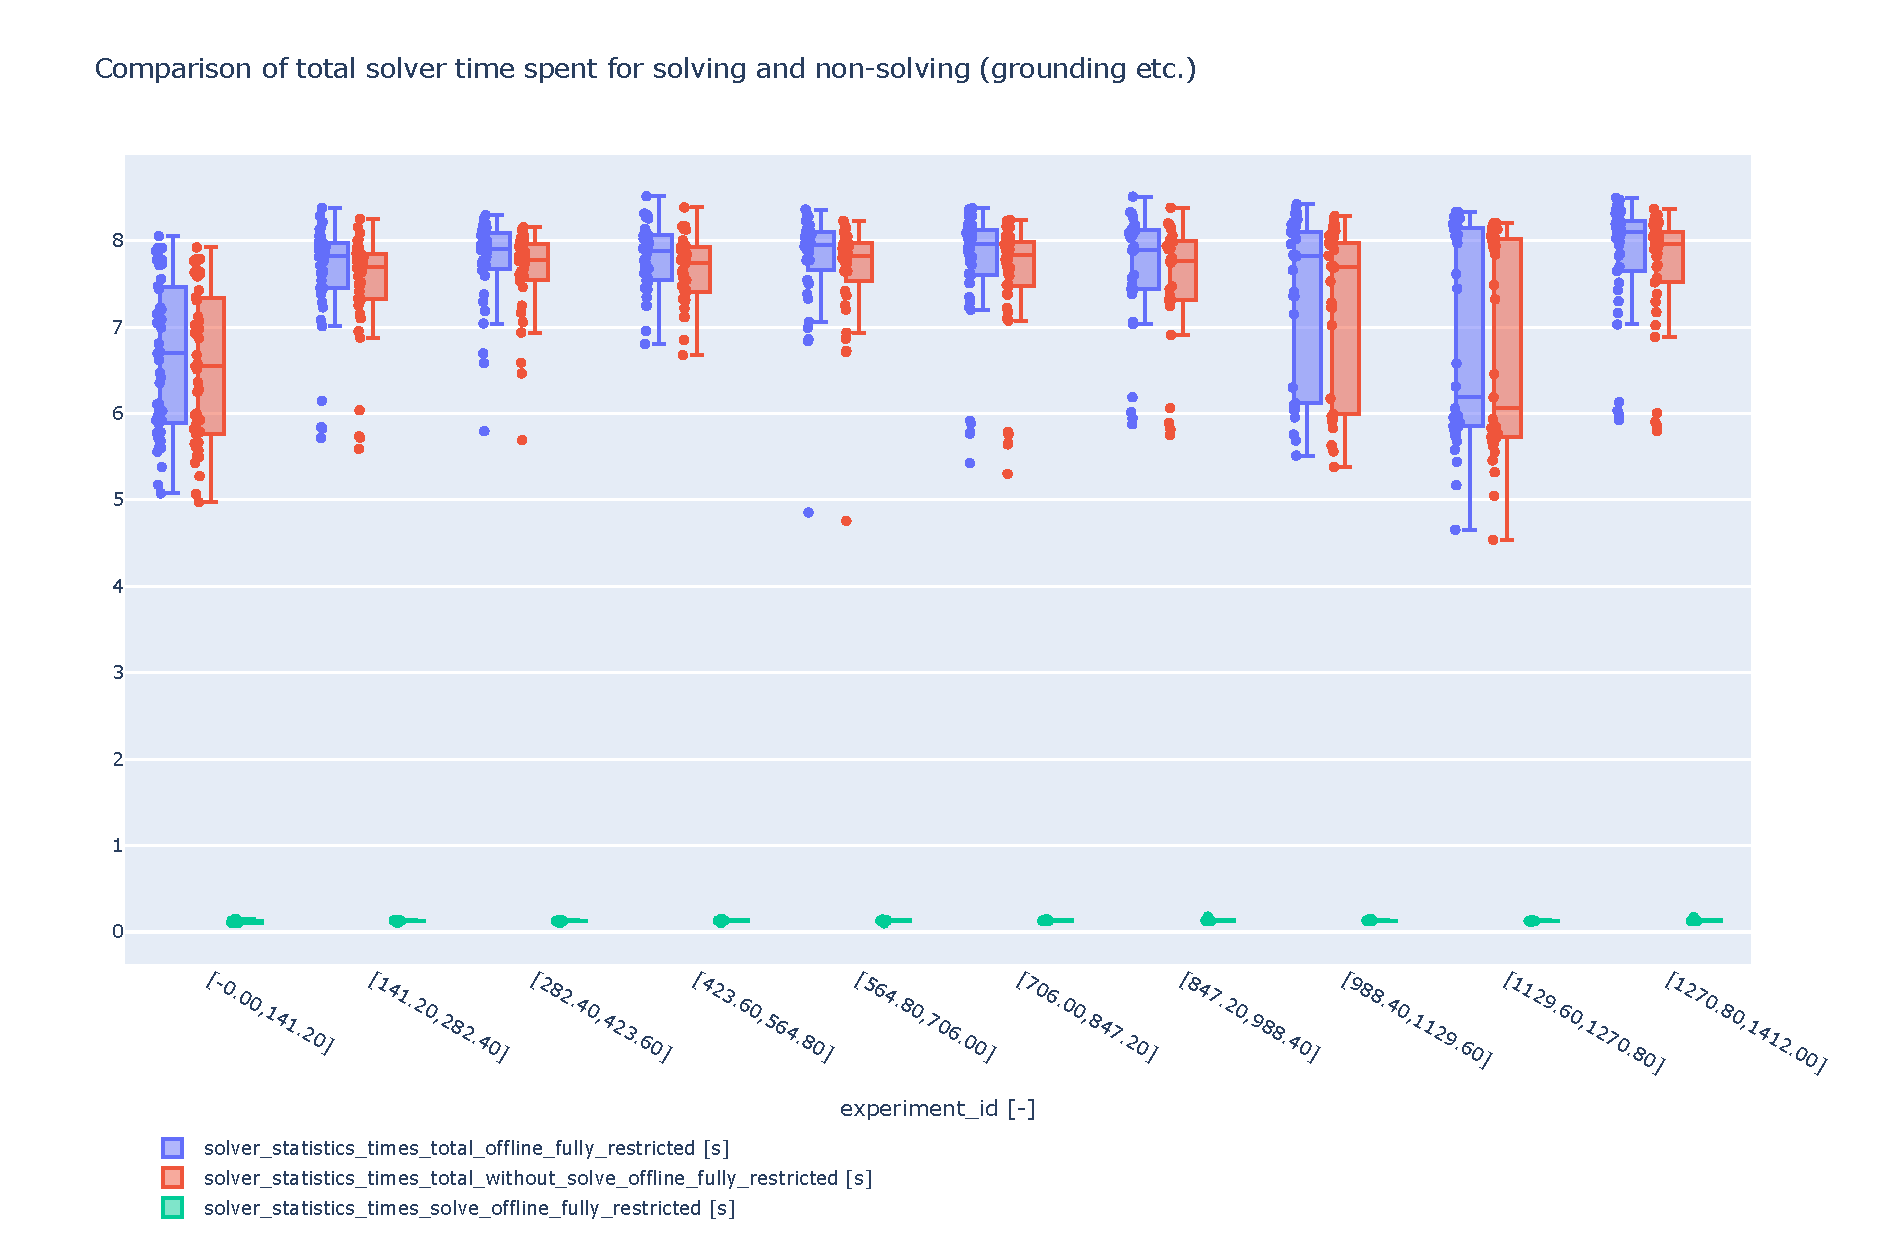
\includegraphics[width=\textwidth]{Figures/04_computational_results/solve_non_solve_offline_fully_restricted.pdf}
        \caption{Total solver time, solve time and non-solve time for online fully restricted}
         \label{fig:computationtimes_solve_non_solve_time_online_fully_restricted}
    \end{subfigure}
    \begin{subfigure}{\textwidth}
        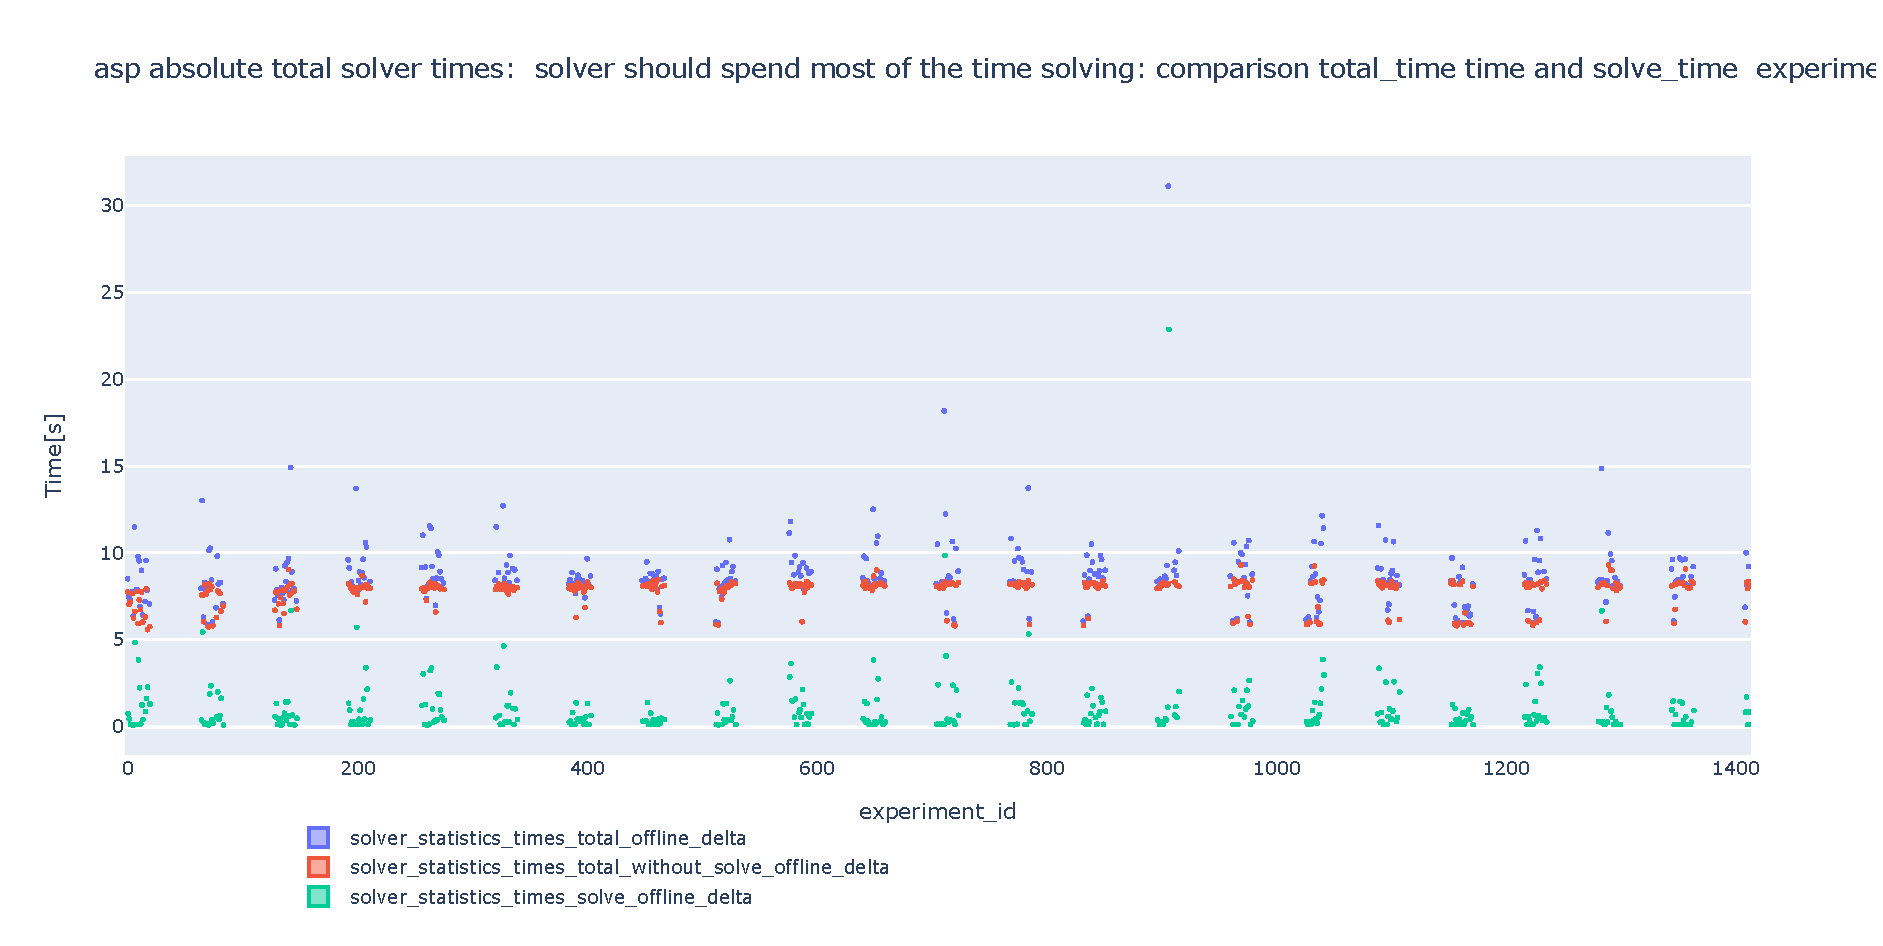
\includegraphics[width=\textwidth]{Figures/04_computational_results/solve_non_solve_offline_delta.pdf}
        \caption{Total solver time, solve time and non-solve time for offline delta}
         \label{fig:computationtimes_solve_non_solve_time_online_delta}
    \end{subfigure}
    \begin{subfigure}{\textwidth}
        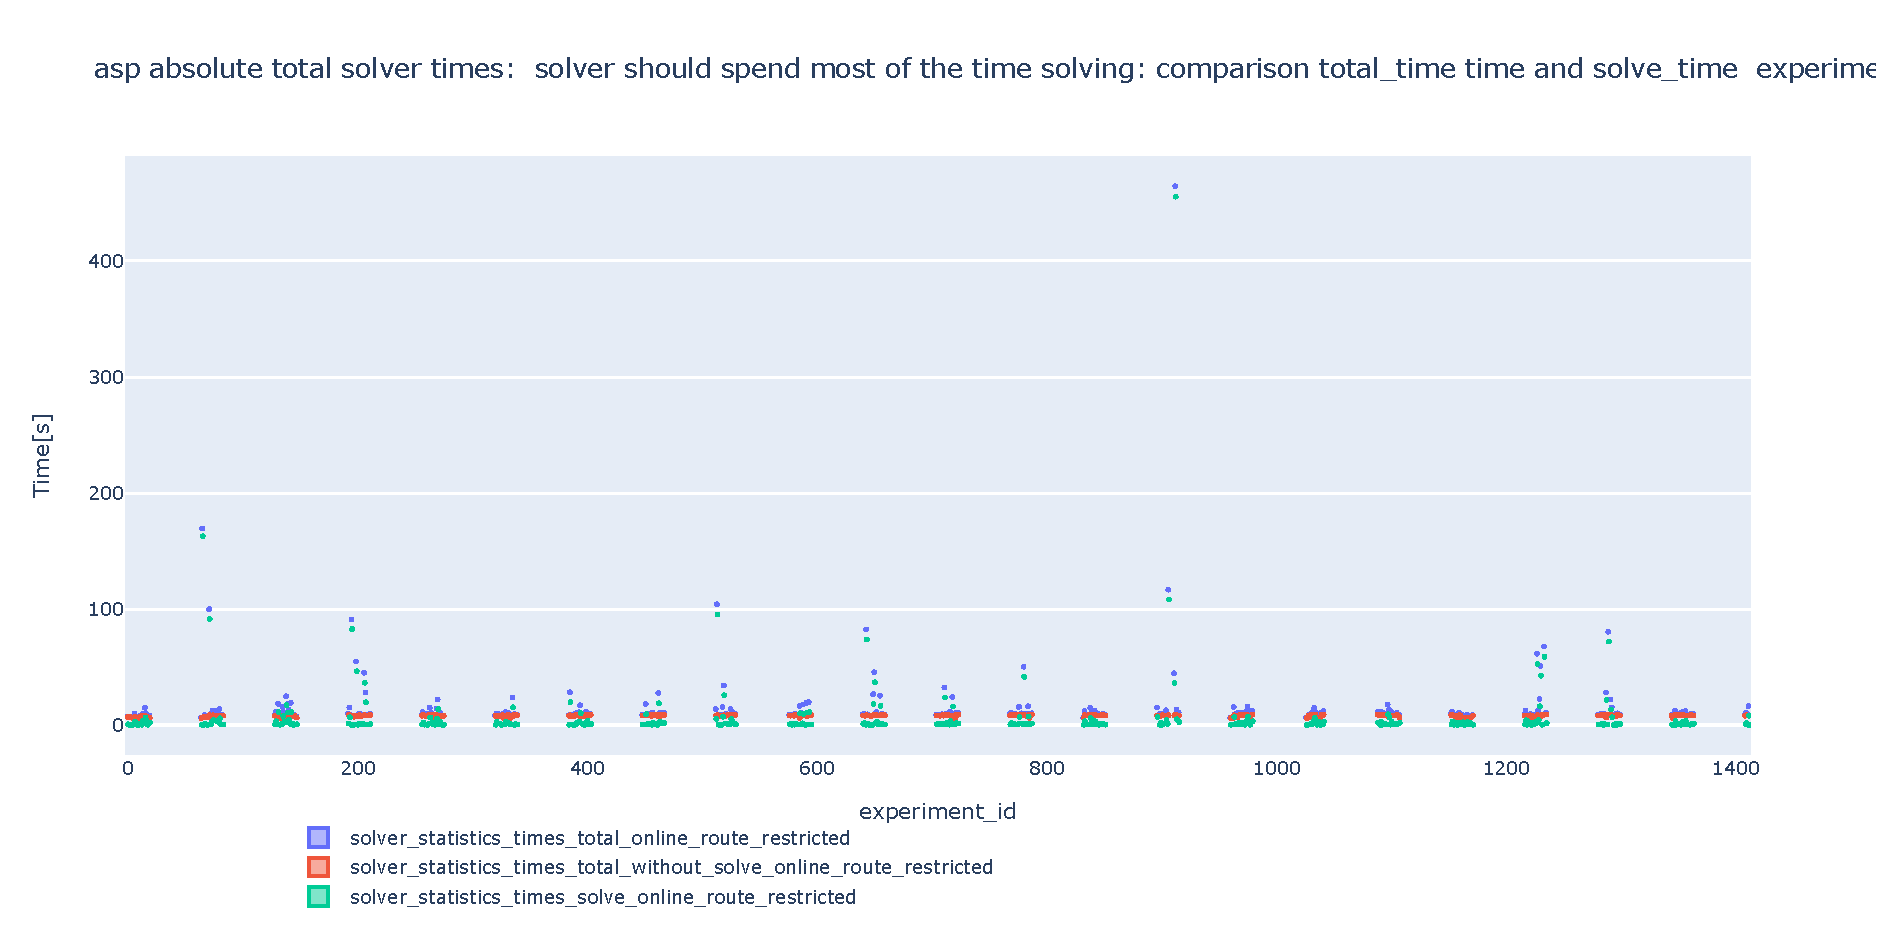
\includegraphics[width=\textwidth]{Figures/04_computational_results/solve_non_solve_online_route_restricted.pdf}
        \caption{Total solver time, solve time and non-solve time for online route restricted}
         \label{fig:computationtimes_solve_non_solve_time_online_route_restricted}
    \end{subfigure}
\end{figure}

\begin{figure}
  \ContinuedFloat
    \begin{subfigure}{\textwidth}
        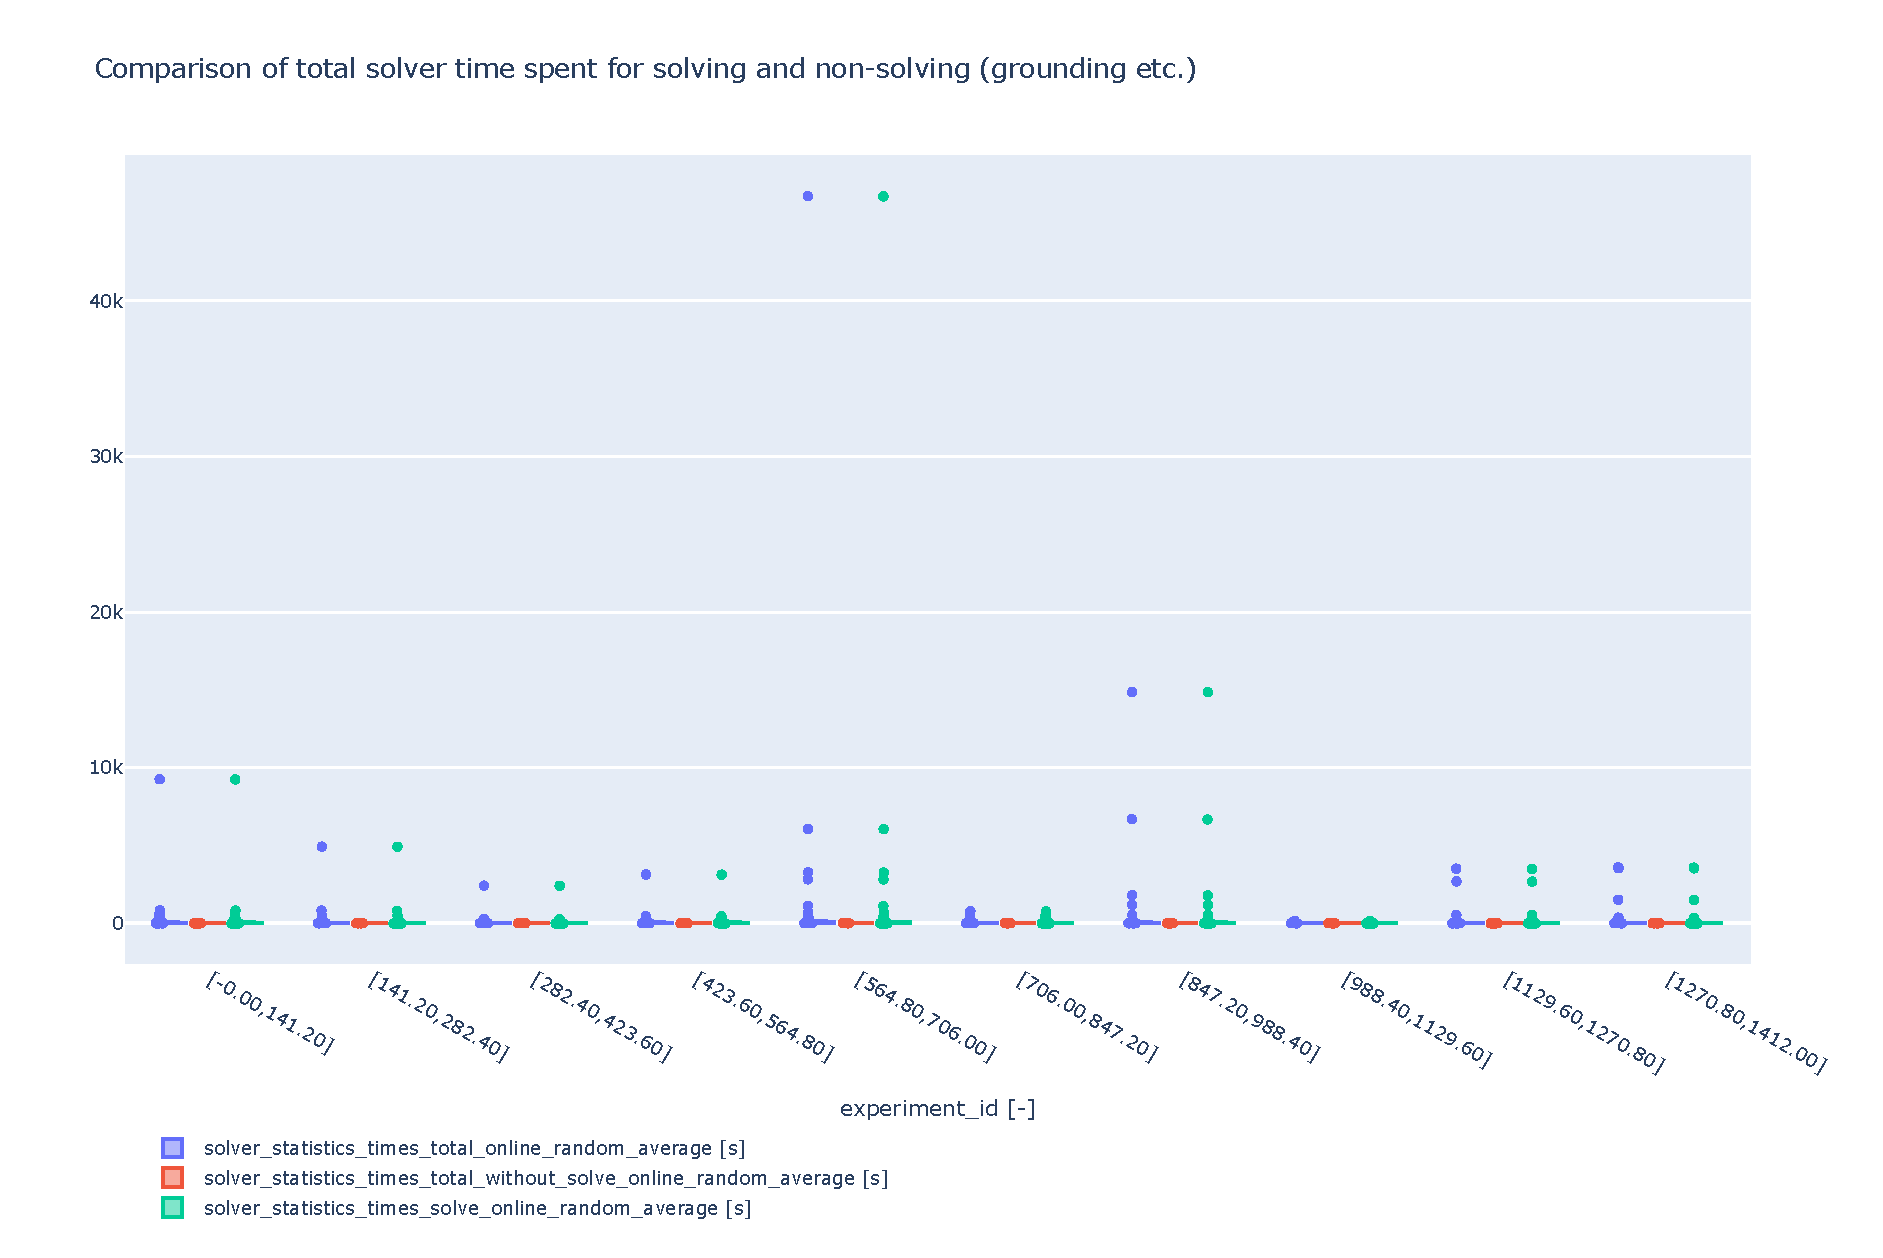
\includegraphics[width=\textwidth]{Figures/04_computational_results/solve_non_solve_online_random_average.pdf}
        \caption{Total solver time, solve time and non-solve time for online random}
         \label{fig:computationtimes_solve_non_solve_time_online_random}
    \end{subfigure}
    \begin{subfigure}{\textwidth}
        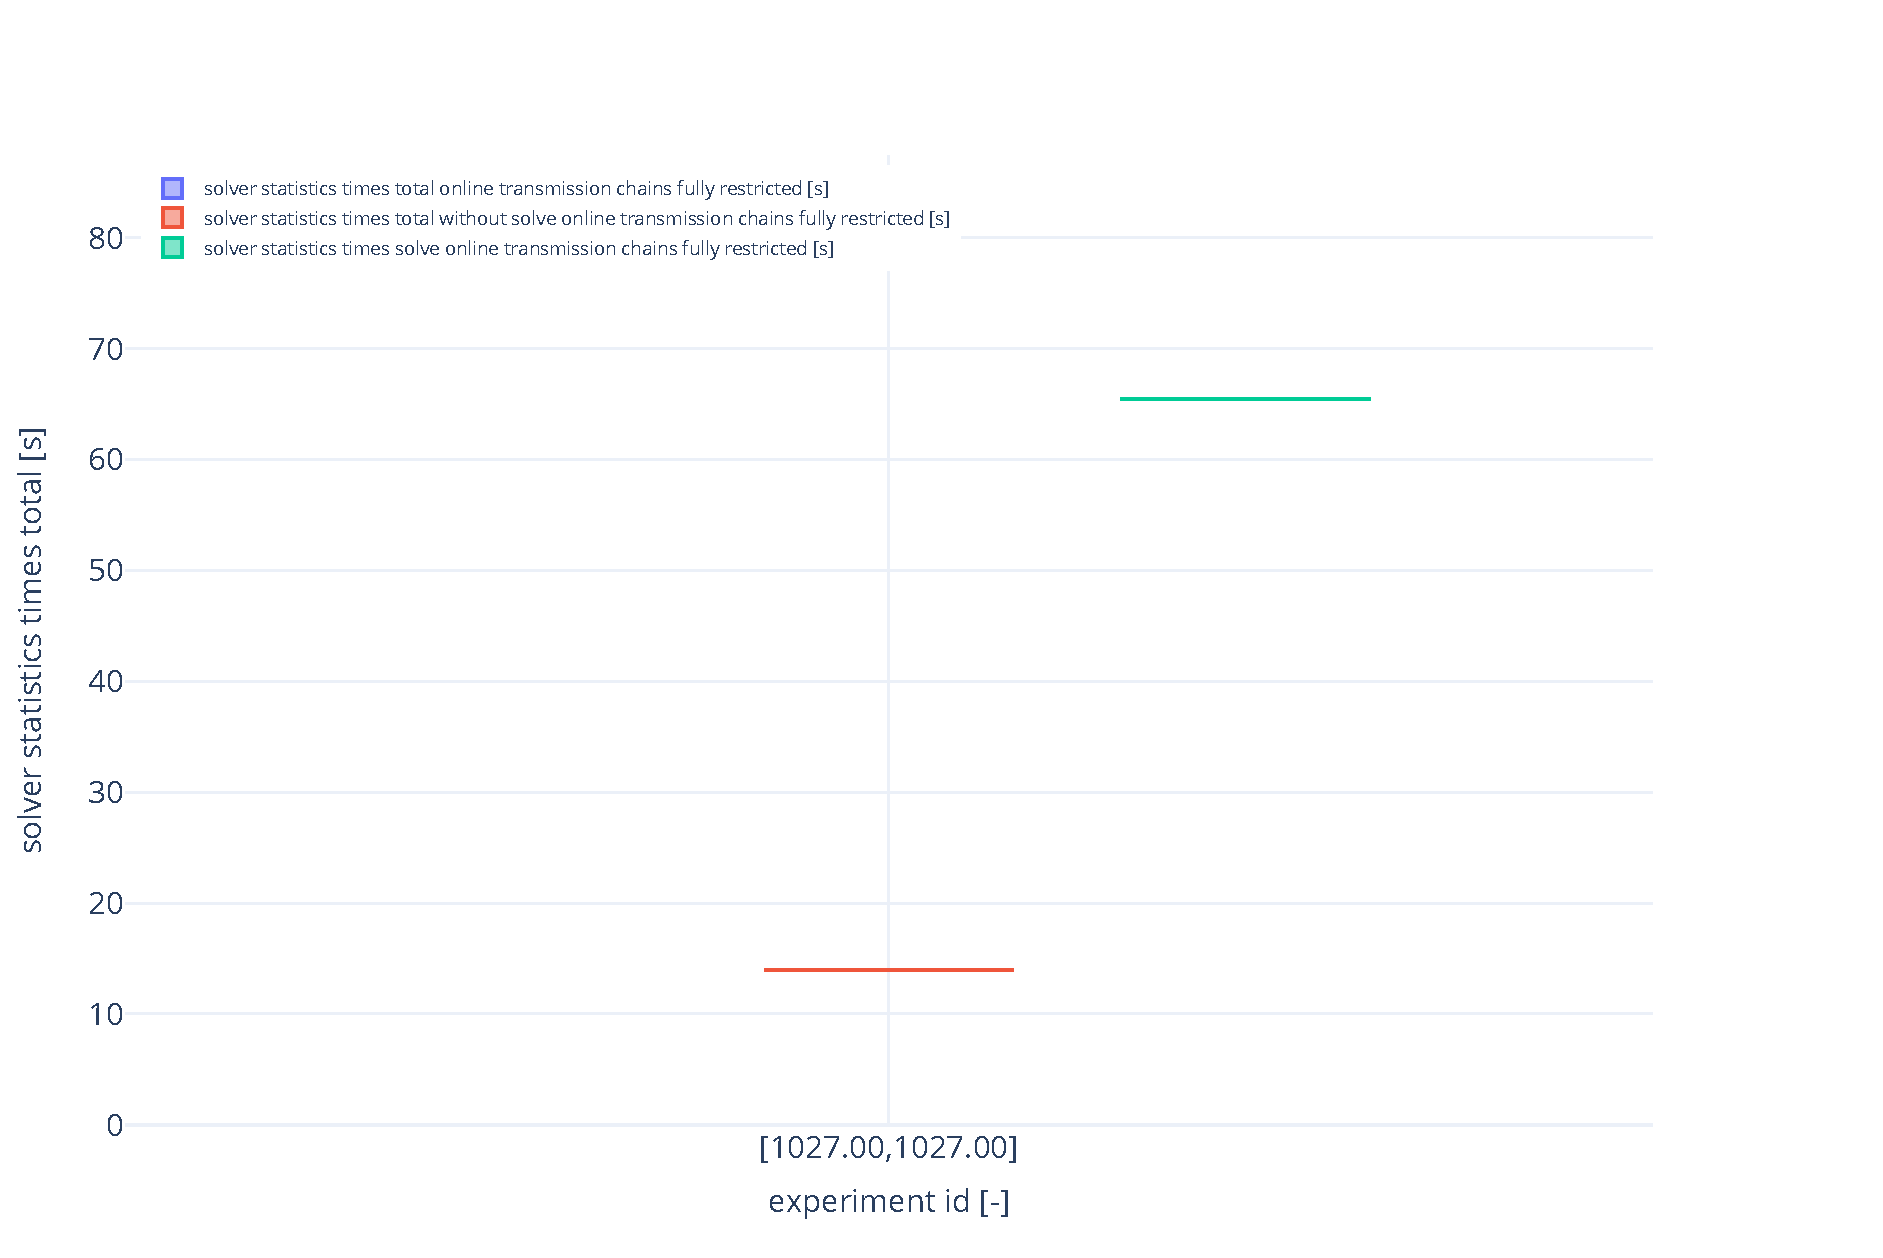
\includegraphics[width=\textwidth]{Figures/04_computational_results/solve_non_solve_online_transmission_chains_fully_restricted.pdf}
                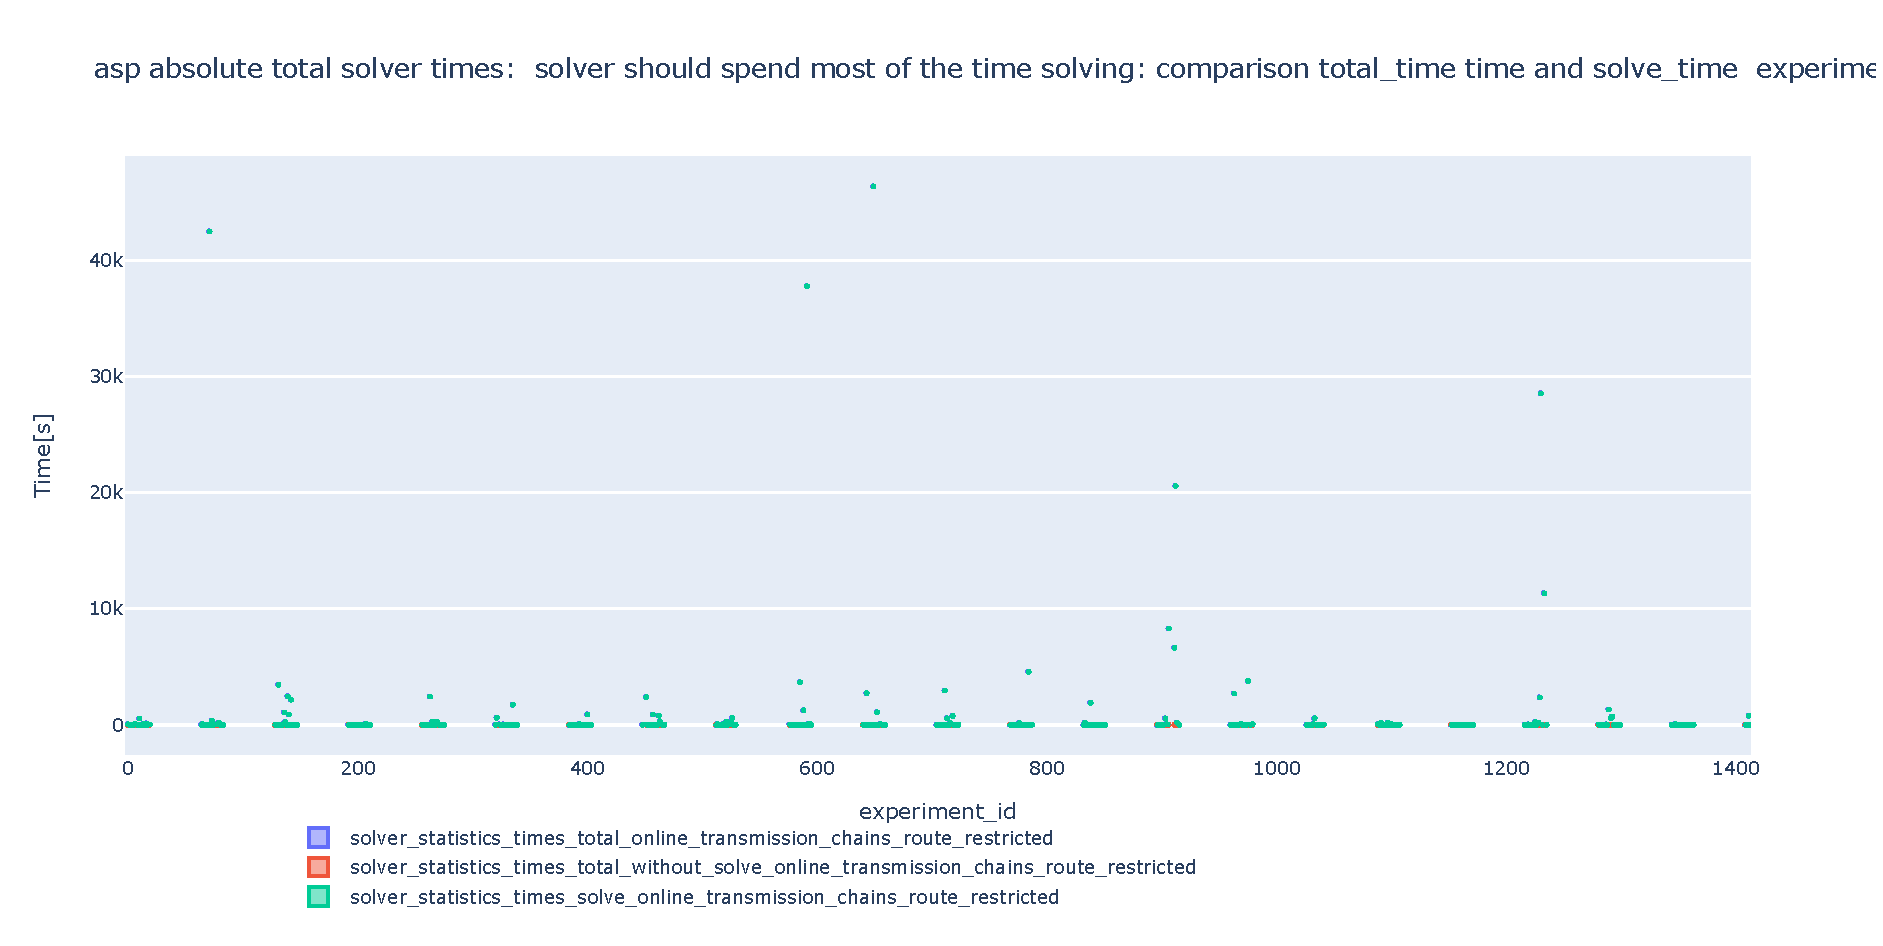
\includegraphics[width=\textwidth]{Figures/04_computational_results/solve_non_solve_online_transmission_chains_route_restricted.pdf}
        \caption{Total solver time, solve time and non-solve time for online transmission chains fully and route restricted}
        \label{fig:computationtimes_solve_non_solve_time_online_tranmission_chains}
    \end{subfigure}
	\caption{Absolute total solver time, solve time and non-solve time of the ASP solver per experiment id.}
	\label{fig:solve_non_solve}
\end{figure}



%%%%%%%%%%%%%%%%%%%%%%%%%%%%%%%%%%%%%%%%%%%%%%%%%%%%%%%%%%%%%%%%%%%%%%%%%%
\subsection{Solution Quality}
%%%%%%%%%%%%%%%%%%%%%%%%%%%%%%%%%%%%%%%%%%%%%%%%%%%%%%%%%%%%%%%%%%%%%%%%%%

Figure~\ref{fig:delay} shows that, as expected, online fully restricted, offline delta yield a solution of the same costs; our transmission chains route restricted also yields the same quality solutions in our experiments\footnote{we do not know whether this is provably so}, only when give the predicted agents no time flexibility (transmission chains fully restricted) does the solution quality slightly deterioriate. Online route restricted incurs additional costs, although it cannot have any routing penalties; the same applies to online random, which randomly chooses the agents having no routing flexibility; our transmission chains scopers seem to lead to good solutions (no additional costs for route restricted, almost no additional costs for fully restricted). There seems to be almost no tradeoff between routing penalties and lateness -- we will come back to this in Section~\ref{sec:CaseStudies}.

\begin{figure}[hbtp]
        \begin{subfigure}{\textwidth}
            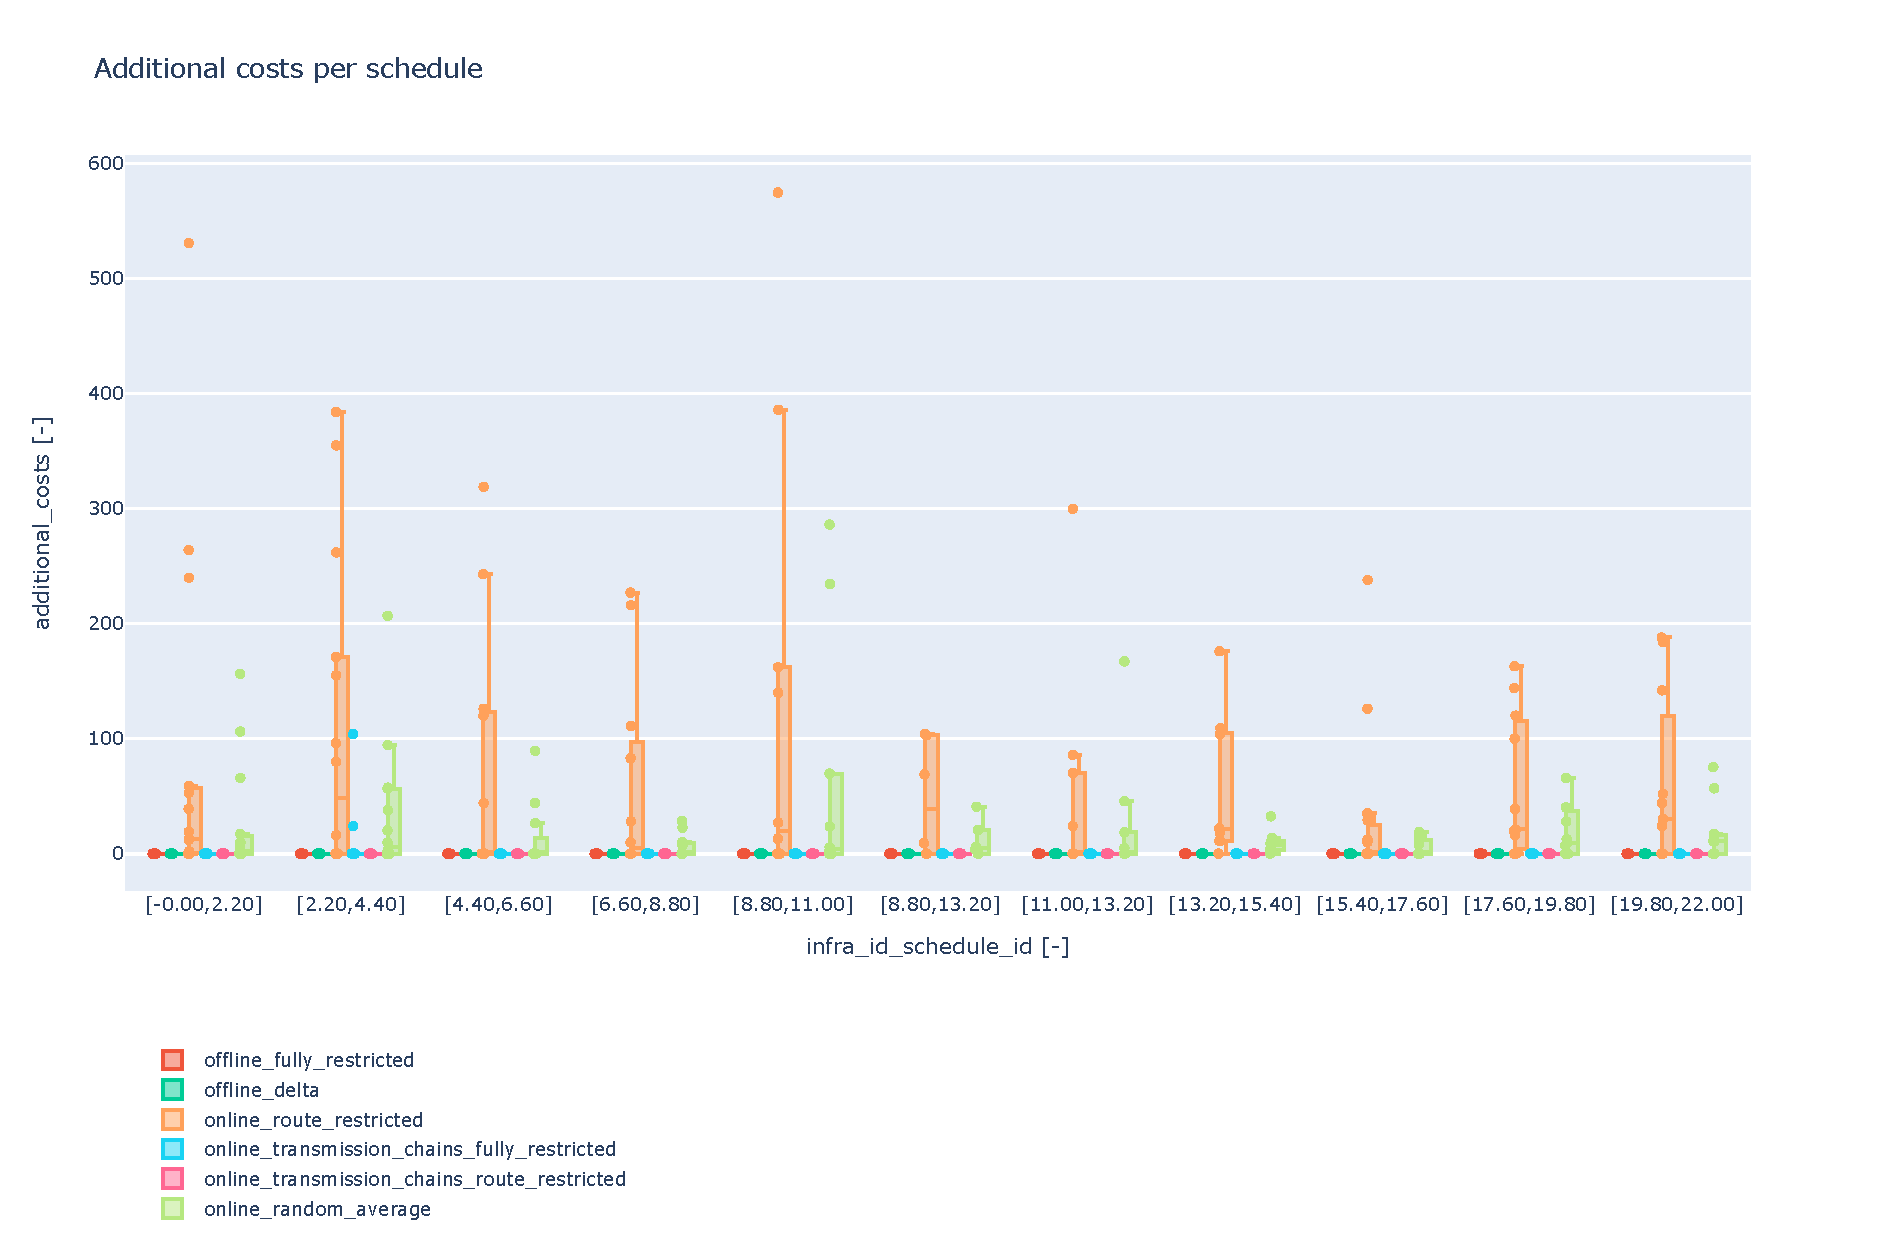
\includegraphics[width=\textwidth]{Figures/04_computational_results/additional_costs.pdf}
            \caption{Additional costs}
             \label{fig:additional_costs}
        \end{subfigure}
        \begin{subfigure}{\textwidth}
            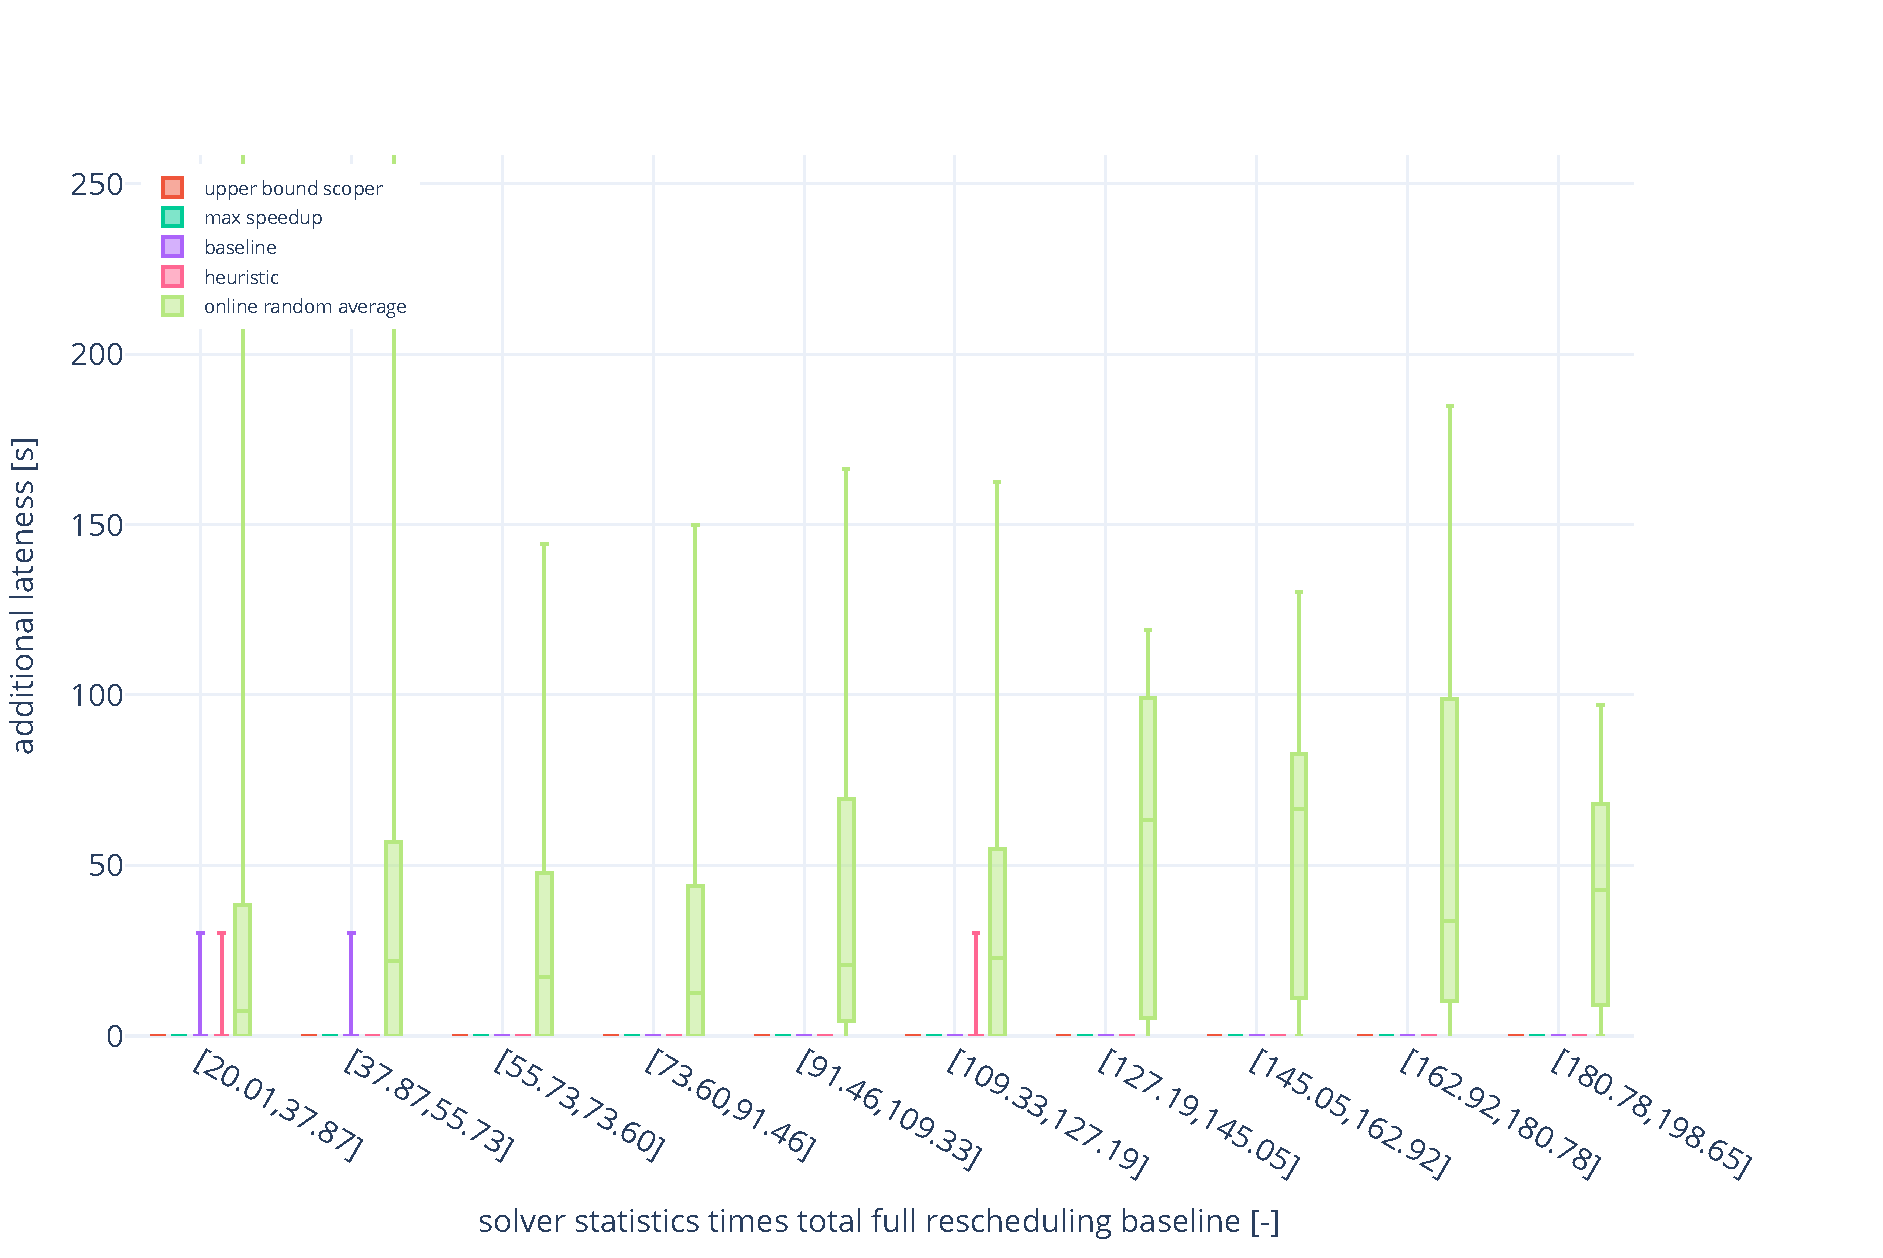
\includegraphics[width=\textwidth]{Figures/04_computational_results/additional_lateness.pdf}
            \caption{Additional lateness}
             \label{fig:additional_lateness}
        \end{subfigure}
        \begin{subfigure}{\textwidth}
            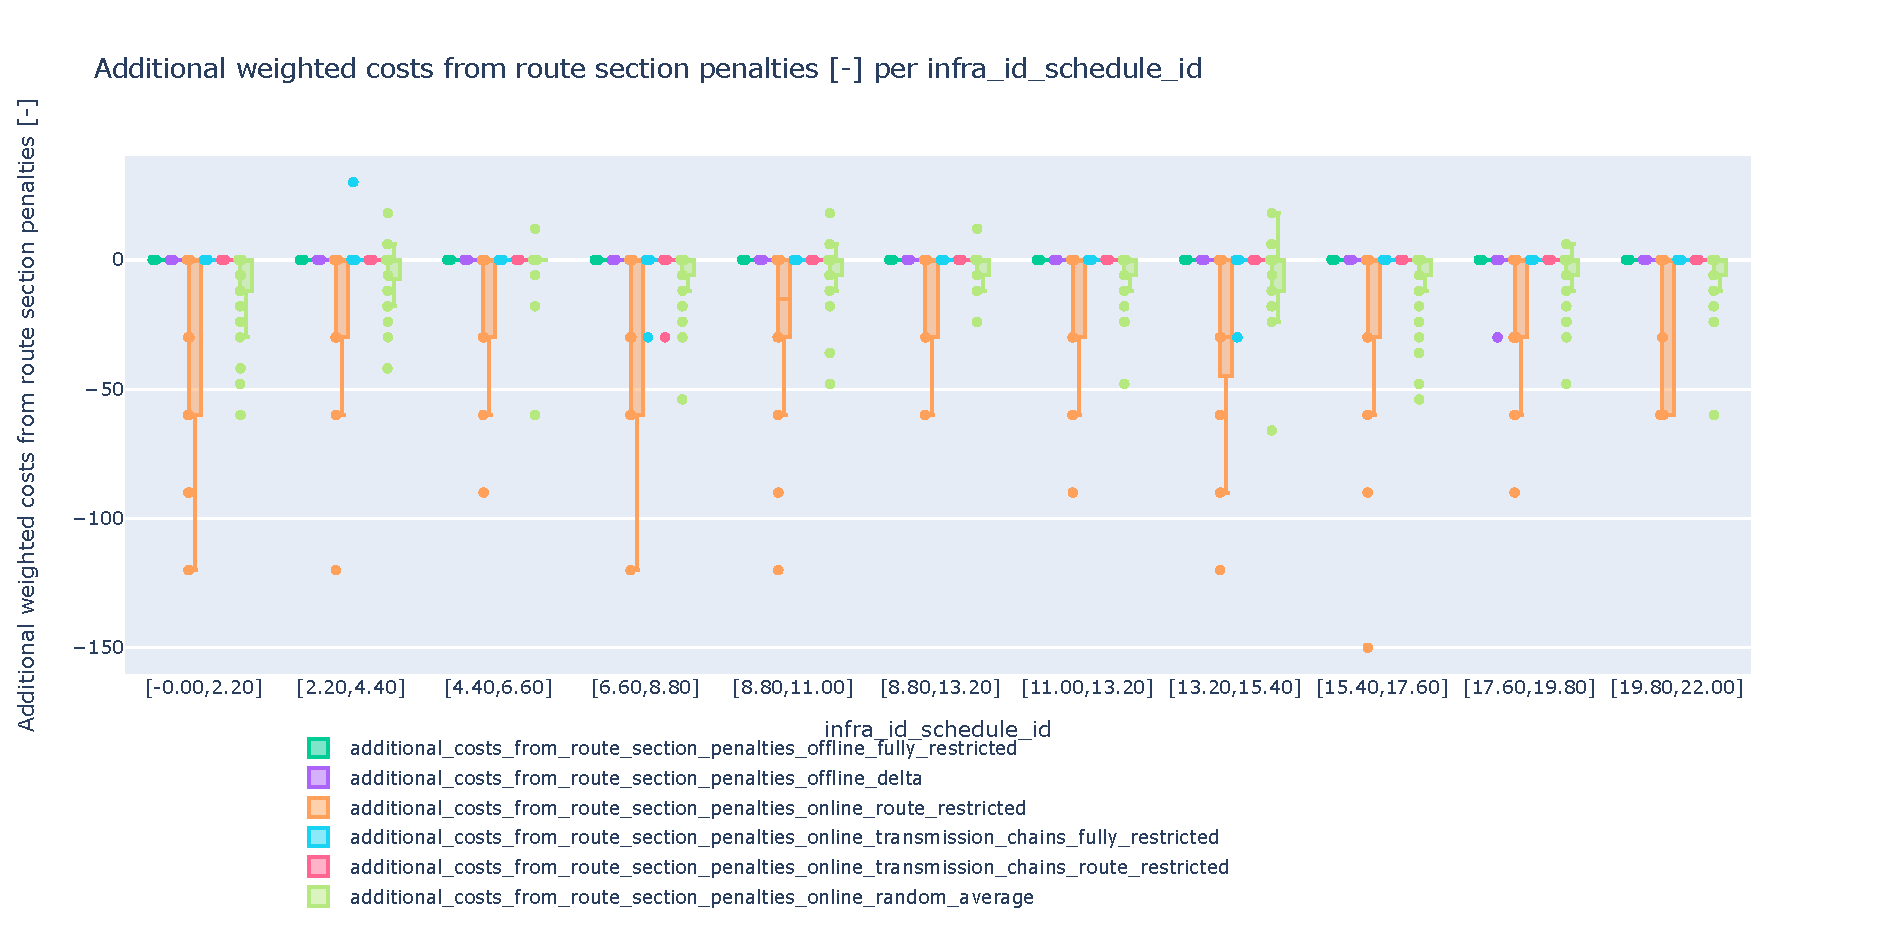
\includegraphics[width=\textwidth]{Figures/04_computational_results/additional_route_section_penalties.pdf}
            \caption{Additional weighted route section penalties}
             \label{fig:additional_route_section_penalties}
        \end{subfigure}
	\caption{Costs per scope.}
	\label{fig:delay}
\end{figure}


%%%%%%%%%%%%%%%%%%%%%%%%%%%%%%%%%%%%%%%%%%%%%%%%%%%%%%%%%%%%%%%%%%%%%%%%%%
\subsection{Prediction Quality}
%%%%%%%%%%%%%%%%%%%%%%%%%%%%%%%%%%%%%%%%%%%%%%%%%%%%%%%%%%%%%%%%%%%%%%%%%%

Figure~\ref{fig:prediction_quality} shows prediction quality for transmission chains and random: our transmission chains scoper has often many false positives, but almost no false negatives

Figure~\ref{fig:additional_changed_agents} shows that online route restricted compensates route restriction by changing more agents than all other scopes, however some experiments seem not to allow for such compensation and less agents are changed at still higher costs as we saw above. It is interesting to see that offline delta changes fewer agents, at the same cost as we saw above -- we will come back to this below in Section~\ref{subsec:cost_equivalence}.

\begin{figure}[hbtp]
    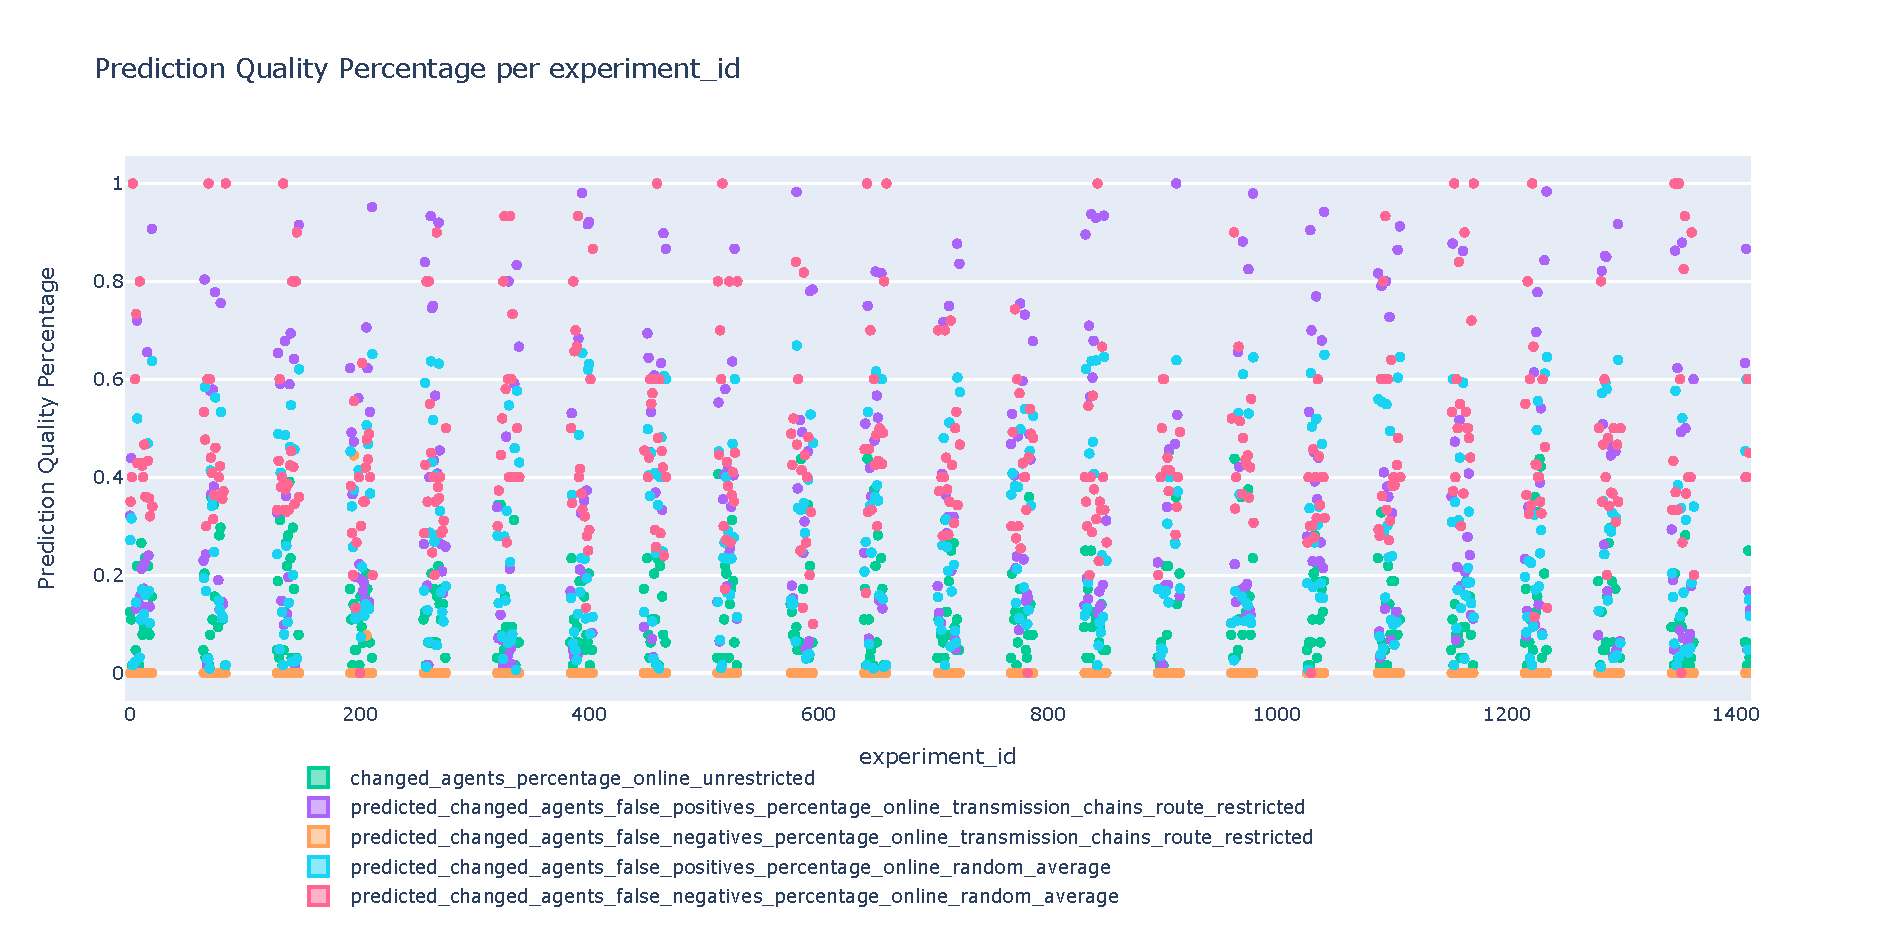
\includegraphics[width=\textwidth]{Figures/04_computational_results/prediction_quality.pdf}
	\caption{Prediction quality: false positives and false negatives rate. Online transmission chains fully restricted is not shown as it is almost completely identical to online transmission chains route restricted.}
	\label{fig:prediction_quality}
\end{figure}

\begin{figure}[hbtp]
    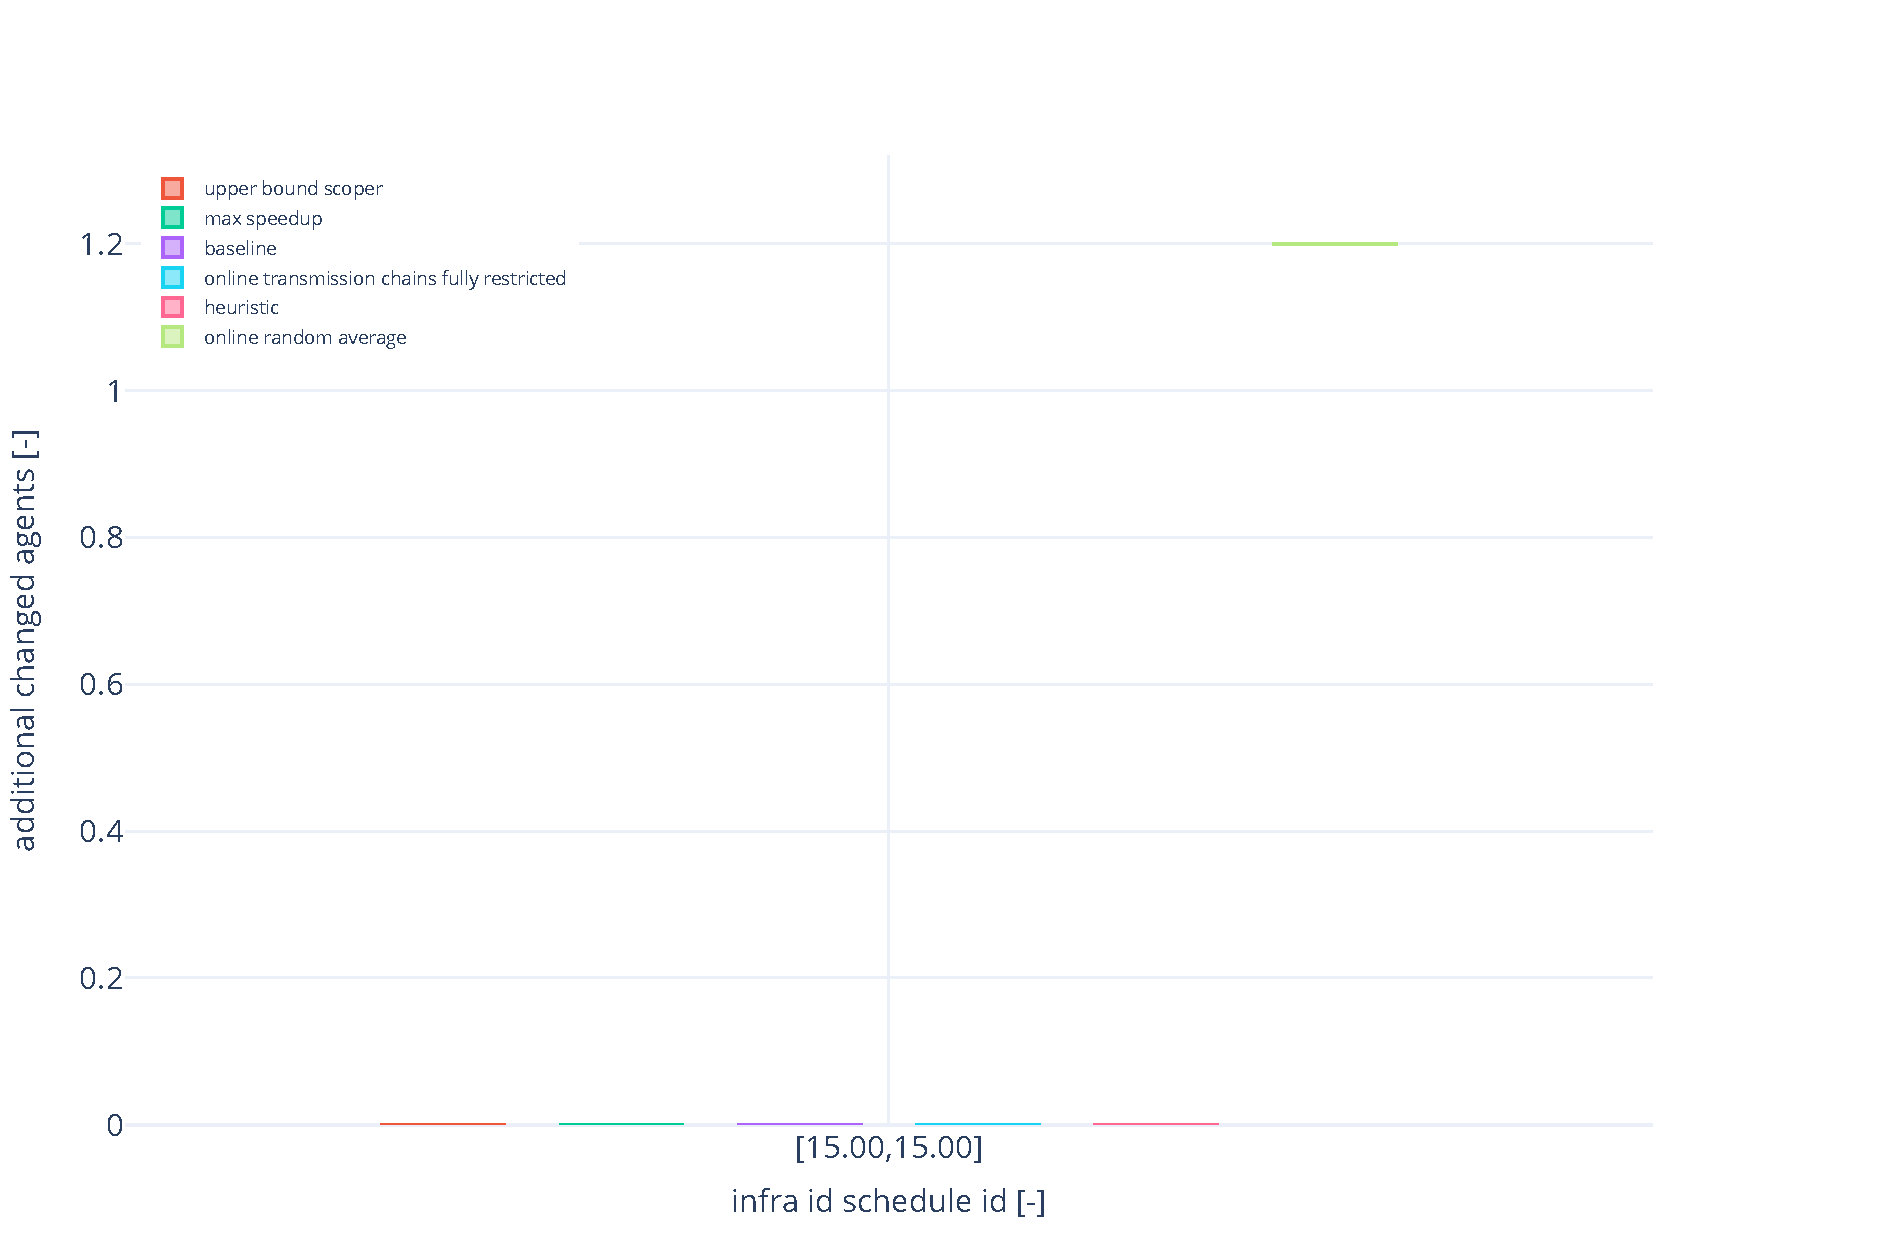
\includegraphics[width=\textwidth]{Figures/04_computational_results/additional_changed_agents.pdf}
	\caption{Additional changed agents.}
	\label{fig:additional_changed_agents}
\end{figure}




%%%%%%%%%%%%%%%%%%%%%%%%%%%%%%%%%%%%%%%%%%%%%%%%%%%%%%%%%%%%%%%%%%%%%%%%%%
\subsection{Discussion}\label{subsec:results_discussion}
%%%%%%%%%%%%%%%%%%%%%%%%%%%%%%%%%%%%%%%%%%%%%%%%%%%%%%%%%%%%%%%%%%%%%%%%%%

On the one hand, the results are good news for our approach since it supports our hypothesis that a huge speed-up is possible, especially if we ignore the non-solve part (we haven't invested in optimizing this part of the model and guess what it could be improved with the ASP solver and that it behaves completely differently with other solvers).

On the other hand, the results must make as also cautious as we compare our  transmission chains approach with online route restricted: our better prediction seems to make it harder for the solver to find solutions in some cases, resulting in much more variance in re-scheduling times than offline delta.

%%%%%%%%%%%%%%%%%%%%%%%%%%%%%%%%%%%%%%%%%%%%%%%%%%%%%%%%%%%%%%%%%%%%%%%%%%
%%%%%%%%%%%%%%%%%%%%%%%%%%%%%%%%%%%%%%%%%%%%%%%%%%%%%%%%%%%%%%%%%%%%%%%%%%
\section{Case Studies}\label{sec:CaseStudies}
%%%%%%%%%%%%%%%%%%%%%%%%%%%%%%%%%%%%%%%%%%%%%%%%%%%%%%%%%%%%%%%%%%%%%%%%%%
%%%%%%%%%%%%%%%%%%%%%%%%%%%%%%%%%%%%%%%%%%%%%%%%%%%%%%%%%%%%%%%%%%%%%%%%%%



%%%%%%%%%%%%%%%%%%%%%%%%%%%%%%%%%%%%%%%%%%%%%%%%%%%%%%%%%%%%%%%%%%%%%%%%%%
\subsection{Cost Equivalence}\label{subsec:cost_equivalence}
%%%%%%%%%%%%%%%%%%%%%%%%%%%%%%%%%%%%%%%%%%%%%%%%%%%%%%%%%%%%%%%%%%%%%%%%%%


We want to illustrate that there are cost equivalent solutions in our setting.
We pick an experiment where we find that the sum of the lateness over all agents and the some over all route section penalties of all agents differ in two scopes, but sum up to the some total costs of the solver. We show such a constellation in Figure~\ref{fig:cost_equivalence_342}.


\begin{figure}[hbtp]
    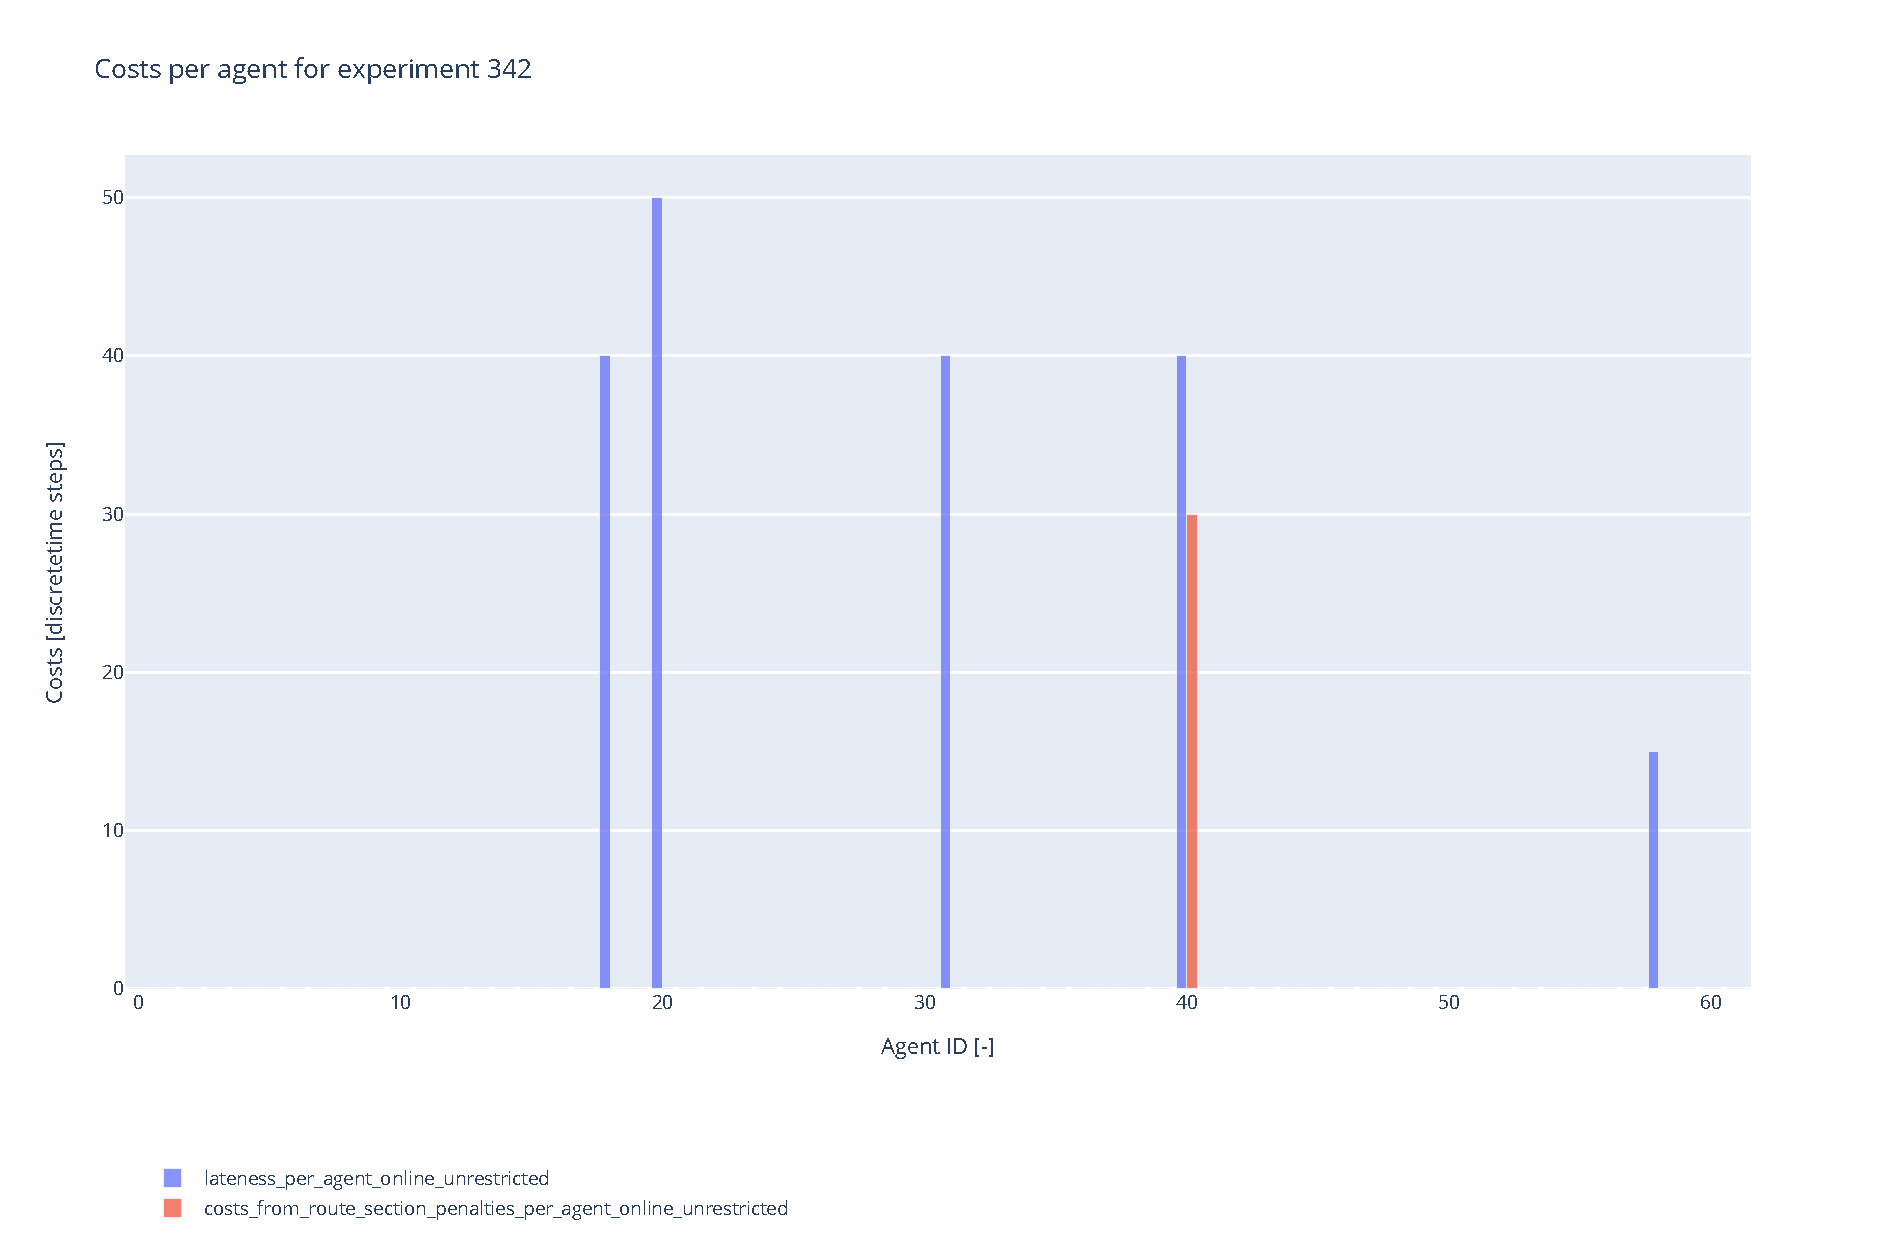
\includegraphics[width=\textwidth]{Figures/05_use_cases/costs_experiment_342.pdf}
	\caption{Illustration of cost equivalence, here one run of experiment $342$ of our agenda (multiple runs may yield different cost equivalent results). Agent $40$ changes route in online unrestricted (penalty $30$), but not in online route restricted, where not changing routes is compensated by a penalty of $10$ for agents  $18$, $31$ and $40$.}
	\label{fig:cost_equivalence_342}
\end{figure}

\begin{mdframed}
{\bf TODO } finalize
\end{mdframed}

The same information is shown in the following table for scopes online\_unrestricted (o.u.) and online\_route\_restricted (o.r.r.):\\
\begin{tabular}{|p{20mm}|p{15mm}|p{20mm}|p{15mm}|p{15mm}|}
\hline
\multirow{2}{*}{\thead{Agent}}  & \multicolumn{2}{c|}{\thead{costs route section penalties}} & \multicolumn{2}{c|}{\thead{online\_route\_restricted}}\\
\cline{2-5} & \thead{o.u.} & \thead{o.r.r.} & \thead{o.u.} & \thead{o.r.r.}\\
\hline
\hline
18 & 40 & 50 & 0 & 0\\
31 & 40 & 50 & 0 & 0 \\
40 & 40 & 50 & 30 & 0\\
% agent 18 has costs differences       online_unrestricted-online_route_restricted
%   lateness                           40 - 50
%   costs_from_route_section_penalties 0 - 0
% agent 18 has changes in range between online_unrestricted and online_route_restricted in range (1552, 1690)
% agent 31 has costs differences       online_unrestricted-online_route_restricted
%   lateness                           40 - 50
%   costs_from_route_section_penalties 0 - 0
% agent 31 has changes in range between online_unrestricted and online_route_restricted in range (1319, 1426)
% agent 40 has costs differences       online_unrestricted-online_route_restricted
%   lateness                           40 - 50
%   costs_from_route_section_penalties 30 - 0
% agent 40 has changes in range between online_unrestricted and online_route_restricted in range (1080, 1675)
% {18: (1552, 1690), 31: (1319, 1426), 40: (1080, 1675)}
% (1080, 1690)
\hline
\end{tabular}
We see that agent $40$ changes route with respect to the initial schedule in o.u., but not in o.r.r.; on the other hand, in o.r.r. all three agents have an additional delay of $10$ time steps compared to o.u. The time resource diagrams for these two situations are shown and discussed in Figure~\ref{fig:cost_equivalence_342_time_resource_diagram}.
\begin{figure}
    \begin{subfigure}{\textwidth}
        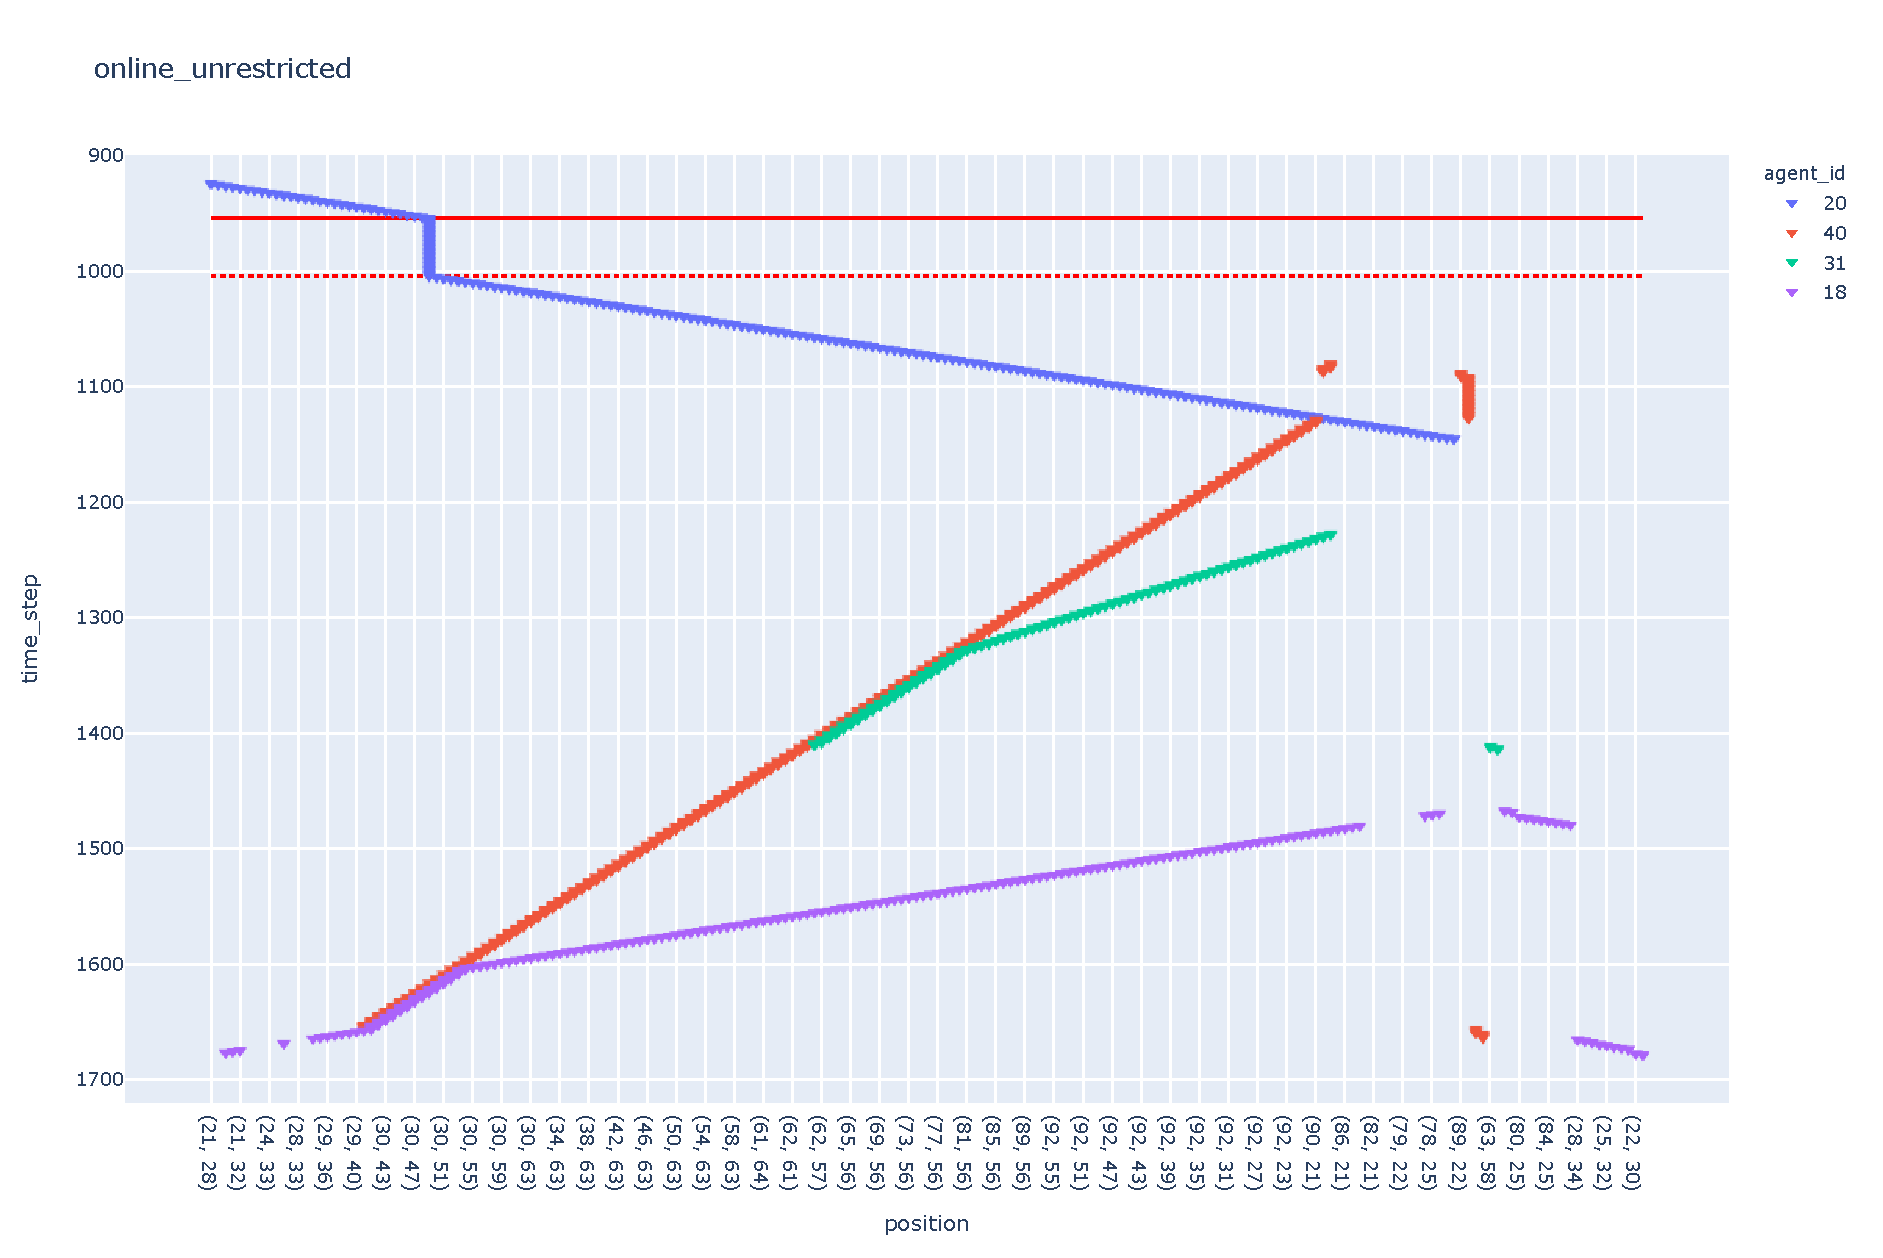
\includegraphics[width=\textwidth]{Figures/05_use_cases/time_resource_online_unrestricted.pdf}
        \label{fig:cost_equivalence_time_resource_online_unrestricted}
        \caption{Time resource diagram for time\_resource\_online\_unrestricted.}
    \end{subfigure}

    \begin{subfigure}{\textwidth}
          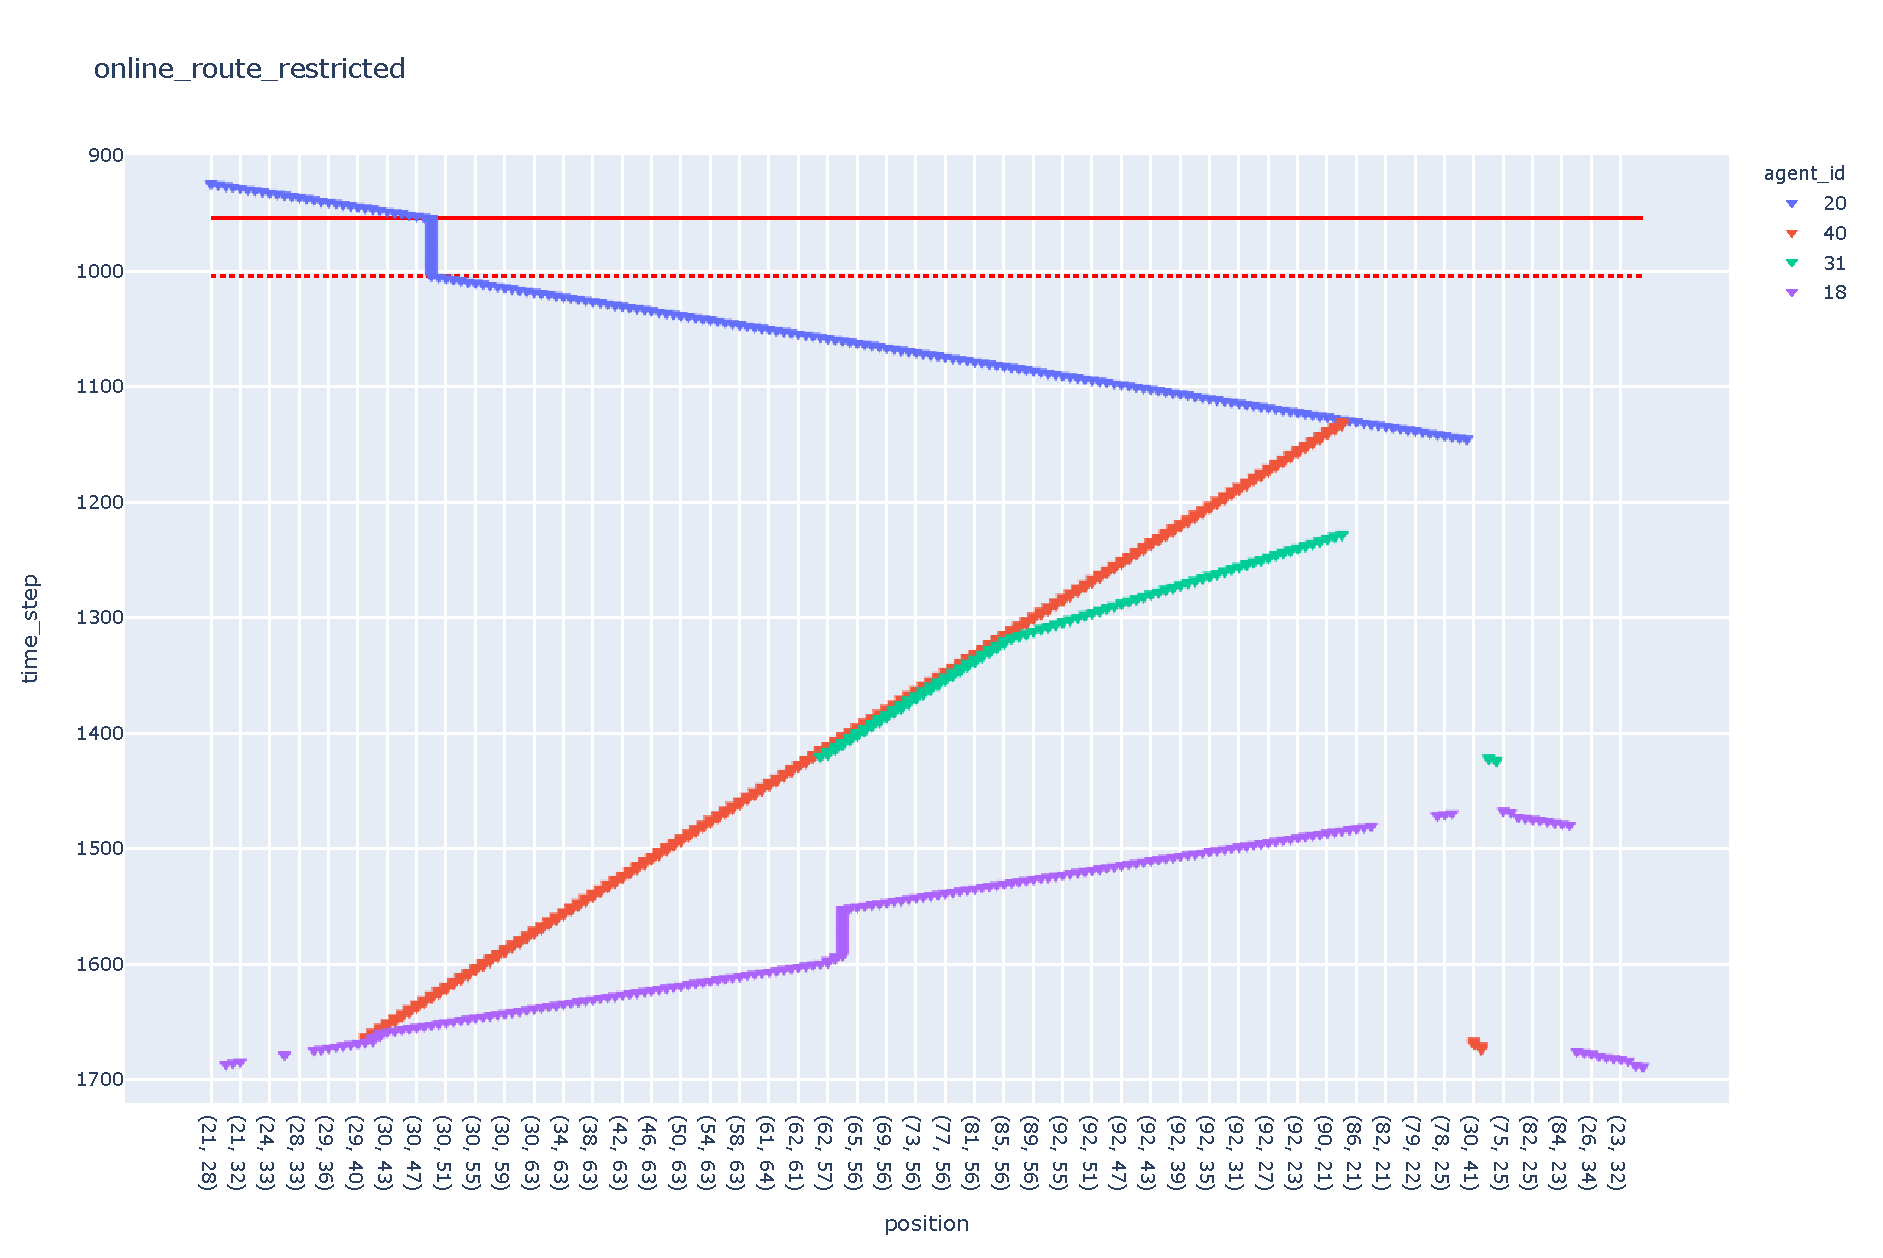
\includegraphics[width=\textwidth]{Figures/05_use_cases/time_resource_online_route_restricted.pdf}
          \label{fig:cost_equivalence_time_resource_online_unrestricted}
          \caption{Time resource diagram for time\_resource\_online\_route\_restricted.}
     \end{subfigure}
	\caption{Time resource diagram two scopes illustrating cost equivalence: Agent $20$ (blue) is the agent having the malfunction at time step $954$ for $50$ time steps (horizontal red line and dashed horizontal red line for malfunction start and end). We see that agent $40$ (red) changes route to start earlier, being delayed but to arrive $10$ time steps earlier in o.u. than in o.r.r. The secondary delay of $10$ time steps of agent $40$ in o.r.r. causes tertiary delay in agents $31$ (green) and $18$ (purple) of $10$ time steps; these two trains are running faster than the red one and catch up. In addition, agent $18$ (purple) has a different behaviour: it does not catch up fully onto agent $40$ (red), but pauses and resumes during its run in o.r.r., staying within time windows of size $60$. The trajectories look as if they overlapped when trains catch up; however, zooming in would should that they do not overlap, the effect being due to the markers for the occupations not being scaled properly.}
	\label{fig:cost_equivalence_342_time_resource_diagram}
\end{figure}

%%%%%%%%%%%%%%%%%%%%%%%%%%%%%%%%%%%%%%%%%%%%%%%%%%%%%%%%%%%%%%%%%%%%%%%%%%
\subsection{False Positives and False Negatives}
%%%%%%%%%%%%%%%%%%%%%%%%%%%%%%%%%%%%%%%%%%%%%%%%%%%%%%%%%%%%%%%%%%%%%%%%%%

\label{subsec:false_positives_false_negatives}
\begin{mdframed}
{\bf TODO } take example of false positive and false negative from online tranmission chains
\end{mdframed}


\subsection{Outlier Example}\label{subsec:outlier}
\begin{mdframed}
{\bf TODO}
\begin{itemize}
    \item very high online unrestricted
    \item very high random average with respect to its bin
    \item ...
\end{itemize}
\end{mdframed}



%%%%%%%%%%%%%%%%%%%%%%%%%%%%%%%%%%%%%%%%%%%%%%%%%%%%%%%%%%%%%%%%%%%%%%%%%%
\subsection{Malfunction Variation}\label{subsec:malfunction_variation}
%%%%%%%%%%%%%%%%%%%%%%%%%%%%%%%%%%%%%%%%%%%%%%%%%%%%%%%%%%%%%%%%%%%%%%%%%%


\begin{mdframed}
{\bf TODO } take a schedule and agent and vary the time of malfunction: show monotone decreasing effect (number of agents affected, re-scheduling time)
\end{mdframed}




%%%%%%%%%%%%%%%%%%%%%%%%%%%%%%%%%%%%%%%%%%%%%%%%%%%%%%%%%%%%%%%%%%%%%%%%%%
%%%%%%%%%%%%%%%%%%%%%%%%%%%%%%%%%%%%%%%%%%%%%%%%%%%%%%%%%%%%%%%%%%%%%%%%%%
\section{Extended Discussion/Related Work/Literature: show links to various Research Approaches}
%%%%%%%%%%%%%%%%%%%%%%%%%%%%%%%%%%%%%%%%%%%%%%%%%%%%%%%%%%%%%%%%%%%%%%%%%%
%%%%%%%%%%%%%%%%%%%%%%%%%%%%%%%%%%%%%%%%%%%%%%%%%%%%%%%%%%%%%%%%%%%%%%%%%%

\begin{mdframed}
{\bf TODO}         ML
        delay propagation / recourse / stability of iterative and batch processing
        simulation
        OR / heuristics (job insertion)
        decomposition approaches
        real-time rescheduling

\end{mdframed}


%%%%%%%%%%%%%%%%%%%%%%%%%%%%%%%%%%%%%%%%%%%%%%%%%%%%%%%%%%%%%%%%%%%%%%%%%%
%%%%%%%%%%%%%%%%%%%%%%%%%%%%%%%%%%%%%%%%%%%%%%%%%%%%%%%%%%%%%%%%%%%%%%%%%%
\section{Conclusion}\label{sec:Conclusion}
%%%%%%%%%%%%%%%%%%%%%%%%%%%%%%%%%%%%%%%%%%%%%%%%%%%%%%%%%%%%%%%%%%%%%%%%%%
%%%%%%%%%%%%%%%%%%%%%%%%%%%%%%%%%%%%%%%%%%%%%%%%%%%%%%%%%%%%%%%%%%%%%%%%%%


\begin{description}
\item[G0] We have a given a formal description of problem scope reduction.
\item[G1] We have given multiple illustration of the malfunction spread and its non-monotonicity in time and space. We therefore think that it is more natural to consider the affected scope in the global scope than to decompose the global problem into geographic regions and iteratively solve the global problem by adapting boundary conditions which make the subproblems independent.
However, we are not sure whether scope reduction is possible if
    \begin{itemize}
        \item the schedule becomes very dense everywhere (delays can nowhere be absorbed or compensated) and the problem therefore might not separate well
        \item the schedule loses regularity and we might therefore not be able to use historic data for scope reduction (we have not tackled
    \end{itemize}
\item[G2] We have shown promising speed-ups with the ASP solver model, however we suspect that behaviour could be significantly different with other solvers (for instance, solvers which do not have an initial grounding phase or solvers that exploit the graph-temporal problem structure better); however, we conjecture that scoping in time and space rather than decomposition could enhance solver times for other techniques as well.
\item[G3] We have shown that the scoping problem is not trivial, by implementing a plausible scoper; however, we have not shown that it is possible to build an efficient online scoper.
\item[G4] We provide an extensible playground open-source implementation. The code quality is acceptable, but lacks the quality to be used as a library in a black box way. We aim at turning our approach into a coding challenge; this could happen
\begin{itemize}
\item as part of the RSP pipeline by generating historic data (multiple malfunction and their re-scheduling) and trying to build an online scoper based on historic data, which not only memorizes the historic solution;
\item as part of FLATland by adding an initial schedule in the sense of a conflict-free detailed operational plan and penalizing delay with respect to the initial schedule, still focussing on a trade-off between computation time and solution quality.
\end{itemize}

\end{description}





%%%%%%%%%%%%%%%%%%%%%%%%%%%%%%%%%%%%%%%%%%%%%%%%%%%%%%%%%%%%%%%%%%%%%%%%%%
%%%%%%%%%%%%%%%%%%%%%%%%%%%%%%%%%%%%%%%%%%%%%%%%%%%%%%%%%%%%%%%%%%%%%%%%%%
%%%%%%%%%%%%%%%%%%%%%%%%%%%%%%%%%%%%%%%%%%%%%%%%%%%%%%%%%%%%%%%%%%%%%%%%%%
\appendix
%%%%%%%%%%%%%%%%%%%%%%%%%%%%%%%%%%%%%%%%%%%%%%%%%%%%%%%%%%%%%%%%%%%%%%%%%%
%%%%%%%%%%%%%%%%%%%%%%%%%%%%%%%%%%%%%%%%%%%%%%%%%%%%%%%%%%%%%%%%%%%%%%%%%%
%%%%%%%%%%%%%%%%%%%%%%%%%%%%%%%%%%%%%%%%%%%%%%%%%%%%%%%%%%%%%%%%%%%%%%%%%%



%%%%%%%%%%%%%%%%%%%%%%%%%%%%%%%%%%%%%%%%%%%%%%%%%%%%%%%%%%%%%%%%%%%%%%%%%%
%%%%%%%%%%%%%%%%%%%%%%%%%%%%%%%%%%%%%%%%%%%%%%%%%%%%%%%%%%%%%%%%%%%%%%%%%%
\section{Model Calibration}\label{subsec:model_calibration}
%%%%%%%%%%%%%%%%%%%%%%%%%%%%%%%%%%%%%%%%%%%%%%%%%%%%%%%%%%%%%%%%%%%%%%%%%%
%%%%%%%%%%%%%%%%%%%%%%%%%%%%%%%%%%%%%%%%%%%%%%%%%%%%%%%%%%%%%%%%%%%%%%%%%%

\begin{mdframed}
{\bf TODO} ASP: preprocessing vs. solving; different parameters (delay model?): which parameters make the problem harder, what do we measure?
\end{mdframed}

\subsection{effect of SEQ heuristic (SIM-167)}

\subsection{effect of delay model resolution with 2, 5, 10 (SIM-542)}

\subsection{effect of --propagate (SIM-543)}






%%%%%%%%%%%%%%%%%%%%%%%%%%%%%%%%%%%%%%%%%%%%%%%%%%%%%%%%%%%%%%%%%%%%%%%%%%
%%%%%%%%%%%%%%%%%%%%%%%%%%%%%%%%%%%%%%%%%%%%%%%%%%%%%%%%%%%%%%%%%%%%%%%%%%
\section{Experiment Parameters}\label{subsec:experiment_parameters}
%%%%%%%%%%%%%%%%%%%%%%%%%%%%%%%%%%%%%%%%%%%%%%%%%%%%%%%%%%%%%%%%%%%%%%%%%%
%%%%%%%%%%%%%%%%%%%%%%%%%%%%%%%%%%%%%%%%%%%%%%%%%%%%%%%%%%%%%%%%%%%%%%%%%%

Here we give the full parameter ranges for the results of Section~\ref{sec:Results}.
Values correspond to \url{https://github.com/SchweizerischeBundesbahnen/rsp-data/tree/master/PUBLICATION_DATA}, generated by \url{https://github.com/SchweizerischeBundesbahnen/rsp/blob/3c92f19f69abc1d8ea5bfc344526cb971e75a118/src/python/rsp/hypothesis_one_experiments_potassco.py}.
The value ranges $[a, b, n]$ have the following meaning:
if $n=1$, we take only $a$; if $n>1$, we take $n-1$ points from the half-open interval $[a,b)$ of step size $step=\lfloor \frac{b-a}{a}\rfloor$; in the following tables, we abbreviate $100$ instead for $[100, 100, 1]$\footnote{We should probably harmonize the implementation and take $n$ points from $[a,b]$ with step size $step$ instead.}.

\subsection{Infrastructure Parameters}

\begin{tabular}{|p{40mm}|p{15mm}|p{40mm}|p{15mm}|}
\hline
\thead{Parameter} & \thead{Symbol} & \thead{Description} & \thead{Value}\\
\hline
\hline
\texttt{infra\_id} & -- & infrastructure id & --\\\hline
\texttt{width} & $w$ & Number of cells in the width of the environment & 100\\\hline
\texttt{height} & $h$ & Number of cells in the height of the environment & 100 \\\hline
\texttt{flatland\_seed\_value} & -- & Random seed to generate different configurations & 190 \\\hline
\texttt{max\_num\_cities} & $\left|S\right|$& Maximum number of cities to be places in the environment. Cities are the only places where agents can start or end their journey. Cities consists of parallel track and entry/exit ports. & $[8, 15, 3]$\\\hline
\texttt{grid\_mode} & -- & & \texttt{False}\\\hline
\texttt{max\_rail\_between\_cities} & -- & Maximum number of parallel track at entry/exit ports of the cities & $[1, 2, 2]$\\\hline
\texttt{max\_rail\_in\_city} & -- & Maximum number of parallel tracks in the city & $[2, 3, 2]$\\
\texttt{number\_of\_agents} & $\left|\mathcal{A}\right|$& & $[50, 100, 4]$\\\hline
\texttt{speed\_data} & $v: \mathcal{A}\to [0,1]$ & distrbution of speeds among agents & \texttt{\{
            1.0: 0.25,
            1.0 / 2.0: 0.25,
            1.0 / 3.0: 0.25,
            1.0 / 4.0: 0.25,
        \}}\\\hline
\texttt{\mbox{number\_of\_shortest\_paths} \mbox{  \_per\_agent}} & $\approx(\mathcal{V}_a,\mathcal{E}_a)$ & We compute shortest paths only once; should be larger than the number in scheduling and re-scheduling.& 10 \\
\hline
\end{tabular}



\subsection{Schedule Parameters}

\begin{tabular}{|p{40mm}|p{15mm}|p{40mm}|p{15mm}|}
\hline
\thead{Parameter} & \thead{Symbol} & \thead{Description} & \thead{Value}\\
\hline\hline
\texttt{infra\_id} & -- & reference to infrastructure & -- \\\hline
\texttt{schedule\_id} & -- & schedule id& --\\\hline
\texttt{asp\_seed\_value} & -- & Since we use 2 threads, the ASP solver behaves non-deterministically, so the seed value has no effect.& $814$ \\\hline
\texttt{number\_of\_shortest\_paths \_per\_agent\_schedule} & $\approx(\mathcal{V}_a,\mathcal{E}_a)$ &  & $1$\\
\hline
\end{tabular}

\subsection{Reschedule Parameters}

\begin{tabular}{|p{40mm}|p{15mm}|p{40mm}|p{15mm}|}
\hline
\thead{Parameter} & \thead{Symbol} & \thead{Description} & \thead{Value}\\
\hline
\hline
\texttt{earliest\_malfunction} & $m_{earliest}$ & Used to determine $m_{time\_step}$, the time step of the malfunction. & $30$\\\hline
\texttt{malfunction\_duration} & $m_{duration}$& Malfunction duration.& $50$\\\hline
\texttt{malfunction\_agent\_id} & $m_{agent}$& Which agent is disturbed? &$[0, 200, 200]$\\\hline
\texttt{number\_of\_shortest\_paths \_per\_agent} & $\approx(S,L)$& Defines the route restrictions for the agents.& $10$\\\hline
\texttt{max\_window\_size\_ from\_earliest} & $c$& Truncate window sizes to this time window sizes to this maximum. Applies to windows on vertices and not on resources. & $30$\\\hline
\texttt{asp\_seed\_value} & -- & Since we use 2 threads, the ASP solver behaves non-deterministically, so the seed value has no effect. &  99\\\hline
\texttt{weight\_route\_change} & $\rho$ & How many time steps delay is one route change equivalent to? & 30 \\\hline
\texttt{weight\_lateness\_seconds} & $\delta_{penalty}$ & Factor to scale delays. Should only be different than $1$ if \texttt{weight\_route\_change} is equal to 1, and vice-versa. & $1$ \\
\hline
\end{tabular}

\section{EF: potential structure for arXiv paper, to be discussed}


\begin{itemize}
    \item Introduction. Motivation (emphasize the setting we aim to address -- one schedule, one infrastructure, historical/simulation data, ...), brief problem description, our conjectures/hypothesis, objectives, literature review (I think it will be short enough to keep it all in the introduction), contributions.
    \item Problem description. Move some of section 1 content here. Also introduce notation for the elements of the system (now in section 3.3). That is the general train re-scheduling problem.
    \item ``Methodology''. What should we call the idea? Train/agent-based scope restriction or something alike. Introduce the idea formally. A general scoper that heuristically restricts the solution space. Discuss guarantees on feasible solution. Issue with false negatives. The link to the solver used for the scheduling problem. The general idea is agnostic to the solver but the performance and implementation hinges on it.
    \item Numerical results
    \begin{itemize}
    \item Experimental design: Flatland, infrastructure/data generation
        \item Scopers in this context
        \item Results
    \end{itemize}
    \item Discussion and outlook: discuss the vision with this approach and the link to machine learning.
    \item Concluding remarks
    \item Acknowledgements (CFF, Mila, ...)
    \item Appendix: all technical details, some of the pseudo codes, ...
\end{itemize}

\bibliographystyle{unsrt}
\bibliography{biblio}

\end{document}
